\documentclass{beamer}

% xcolor and define colors -------------------------
\usepackage{xcolor}

% https://www.viget.com/articles/color-contrast/
\definecolor{purple}{HTML}{5601A4}
\definecolor{navy}{HTML}{0D3D56}
\definecolor{ruby}{HTML}{9a2515}
\definecolor{alice}{HTML}{107895}
\definecolor{daisy}{HTML}{EBC944}
\definecolor{coral}{HTML}{F26D21}
\definecolor{kelly}{HTML}{829356}
\definecolor{cranberry}{HTML}{E64173}
\definecolor{jet}{HTML}{131516}
\definecolor{asher}{HTML}{555F61}
\definecolor{slate}{HTML}{314F4F}

% Mixtape Sessions
\definecolor{picton-blue}{HTML}{00b7ff}
\definecolor{violet-red}{HTML}{ff3881}
\definecolor{sun}{HTML}{ffaf18}
\definecolor{electric-violet}{HTML}{871EFF}

\newcommand\pictonBlue[1]{{\color{picton-blue}#1}}
\newcommand\sun[1]{{\color{sun}#1}}
\newcommand\electricViolet[1]{{\color{electric-violet}#1}}
\newcommand\violetRed[1]{{\color{violet-red}#1}}

\newcommand\bgPictonBlue[1]{{\colorbox{picton-blue!20!white}{#1}}}
\newcommand\bgSun[1]{{\colorbox{sun!20!white}{#1}}}
\newcommand\bgElectricViolet[1]{{\colorbox{electric-violet!20!white}{#1}}}
\newcommand\bgVioletRed[1]{{\colorbox{violet-red!20!white}{#1}}}

\def\code#1{\texttt{#1}}

% Main theme colors
\definecolor{accent}{HTML}{00b7ff}
\definecolor{accent2}{HTML}{871EFF}
\definecolor{gray100}{HTML}{f3f4f6}
\definecolor{gray800}{HTML}{1F292D}


% Beamer Options -------------------------------------

% Background
\setbeamercolor{background canvas}{bg = white}

% Change text margins
\setbeamersize{text margin left = 15pt, text margin right = 15pt} 

% \alert
\setbeamercolor{alerted text}{fg = accent2}

% Frame title
\setbeamercolor{frametitle}{bg = white, fg = jet}
\setbeamercolor{framesubtitle}{bg = white, fg = accent}
\setbeamerfont{framesubtitle}{size = \small, shape = \itshape}

% Block
\setbeamercolor{block title}{fg = white, bg = accent2}
\setbeamercolor{block body}{fg = gray800, bg = gray100}

% Title page
\setbeamercolor{title}{fg = gray800}
\setbeamercolor{subtitle}{fg = accent}

%% Custom \maketitle and \titlepage
\setbeamertemplate{title page}
{
    %\begin{centering}
        \vspace{20mm}
        {\Large \usebeamerfont{title}\usebeamercolor[fg]{title}\inserttitle}\\
        {\large \itshape \usebeamerfont{subtitle}\usebeamercolor[fg]{subtitle}\insertsubtitle}\\ \vspace{10mm}
        {\insertauthor}\\
        {\color{asher}\small{\insertdate}}\\
    %\end{centering}
}

% Table of Contents
\setbeamercolor{section in toc}{fg = accent!70!jet}
\setbeamercolor{subsection in toc}{fg = jet}

% Button 
\setbeamercolor{button}{bg = accent}

% Remove navigation symbols
\setbeamertemplate{navigation symbols}{}

% Table and Figure captions
\setbeamercolor{caption}{fg=jet!70!white}
\setbeamercolor{caption name}{fg=jet}
\setbeamerfont{caption name}{shape = \itshape}

% Bullet points

%% Fix spacing between items
\let\olditemize=\itemize 
\let\endolditemize=\enditemize 
\renewenvironment{itemize}{\vspace{0.25em}\olditemize \itemsep0.25em}{\endolditemize}

%% Fix left-margins
\settowidth{\leftmargini}{\usebeamertemplate{itemize item}}
\addtolength{\leftmargini}{\labelsep}

%% enumerate item color
\setbeamercolor{enumerate item}{fg = accent}
\setbeamerfont{enumerate item}{size = \small}
\setbeamertemplate{enumerate item}{\insertenumlabel.}

%% itemize
\setbeamercolor{itemize item}{fg = accent!70!white}
\setbeamerfont{itemize item}{size = \small}
\setbeamertemplate{itemize item}[circle]

%% right arrow for subitems
\setbeamercolor{itemize subitem}{fg = accent!60!white}
\setbeamerfont{itemize subitem}{size = \small}
\setbeamertemplate{itemize subitem}{$\rightarrow$}

\setbeamertemplate{itemize subsubitem}[square]
\setbeamercolor{itemize subsubitem}{fg = jet}
\setbeamerfont{itemize subsubitem}{size = \small}








% Links ----------------------------------------------

\usepackage{hyperref}
\hypersetup{
  colorlinks = true,
  linkcolor = accent2,
  filecolor = accent2,
  urlcolor = accent2,
  citecolor = accent2,
}


% Line spacing --------------------------------------
\usepackage{setspace}
\setstretch{1.35}


% \begin{columns} -----------------------------------
\usepackage{multicol}


% Fonts ---------------------------------------------
% Beamer Option to use custom fonts
\usefonttheme{professionalfonts}

% \usepackage[utopia, smallerops, varg]{newtxmath}
% \usepackage{utopia}
\usepackage[sfdefault,light]{roboto}

% Small adjustments to text kerning
\usepackage{microtype}



% Remove annoying over-full box warnings -----------
\vfuzz2pt 
\hfuzz2pt


% Table of Contents with Sections
\setbeamerfont{myTOC}{series=\bfseries, size=\Large}
\AtBeginSection[]{
        \frame{
            \frametitle{Roadmap}
            \tableofcontents[current]   
        }
    }


% Tables -------------------------------------------
% Tables too big
% \begin{adjustbox}{width = 1.2\textwidth, center}
\usepackage{adjustbox}
\usepackage{array}
\usepackage{threeparttable, booktabs, adjustbox}
    
% Fix \input with tables
% \input fails when \\ is at end of external .tex file
\makeatletter
\let\input\@@input
\makeatother

% Tables too narrow
% \begin{tabularx}{\linewidth}{cols}
% col-types: X - center, L - left, R -right
% Relative scale: >{\hsize=.8\hsize}X/L/R
\usepackage{tabularx}
\newcolumntype{L}{>{\raggedright\arraybackslash}X}
\newcolumntype{R}{>{\raggedleft\arraybackslash}X}
\newcolumntype{C}{>{\centering\arraybackslash}X}

% Figures

% \imageframe{img_name} -----------------------------
% from https://github.com/mattjetwell/cousteau
\newcommand{\imageframe}[1]{%
    \begin{frame}[plain]
        \begin{tikzpicture}[remember picture, overlay]
            \node[at = (current page.center), xshift = 0cm] (cover) {%
                \includegraphics[keepaspectratio, width=\paperwidth, height=\paperheight]{#1}
            };
        \end{tikzpicture}
    \end{frame}%
}

% subfigures
\usepackage{subfigure}


% Highlight slide -----------------------------------
% \begin{transitionframe} Text \end{transitionframe}
% from paulgp's beamer tips
\newenvironment{transitionframe}{
    \setbeamercolor{background canvas}{bg=accent!40!black}
    \begin{frame}\color{accent!10!white}\LARGE\centering
}{
    \end{frame}
}


% Table Highlighting --------------------------------
% Create top-left and bottom-right markets in tabular cells with a unique matching id and these commands will outline those cells
\usepackage[beamer,customcolors]{hf-tikz}
\usetikzlibrary{calc}
\usetikzlibrary{fit,shapes.misc}

% To set the hypothesis highlighting boxes red.
\newcommand\marktopleft[1]{%
    \tikz[overlay,remember picture] 
        \node (marker-#1-a) at (0,1.5ex) {};%
}
\newcommand\markbottomright[1]{%
    \tikz[overlay,remember picture] 
        \node (marker-#1-b) at (0,0) {};%
    \tikz[accent!80!jet, ultra thick, overlay, remember picture, inner sep=4pt]
        \node[draw, rectangle, fit=(marker-#1-a.center) (marker-#1-b.center)] {};%
}


% DAGS ----------------------------------------------
\usepackage{tikz}
\usetikzlibrary{shapes,decorations,arrows,calc,arrows.meta,fit,positioning}
% Tikz settings optimized for causal graphs.
\tikzset{
    -Latex,auto,node distance =1 cm and 1 cm,semithick,
    state/.style ={ellipse, draw, minimum width = 0.7 cm},
    point/.style = {circle, draw, inner sep=0.04cm,fill,node contents={}},
    bidirected/.style={Latex-Latex,dashed},
    el/.style = {inner sep=2pt, align=left, sloped}
}


% Beamer tricks -------------------------------------
% Make \pause work in align environments
\makeatletter
\renewrobustcmd{\beamer@@pause}[1][]{%
  \unless\ifmeasuring@%
  \ifblank{#1}%
    {\stepcounter{beamerpauses}}%
    {\setcounter{beamerpauses}{#1}}%
  \onslide<\value{beamerpauses}->\relax%
  \fi%
}
\makeatother

\usepackage{breqn} % Breaks lines

\usepackage{amsmath}
\usepackage{mathtools}

\usepackage{pdfpages} % \includepdf

\usepackage{listings} % R code
\usepackage{verbatim} % verbatim

% Video stuff
\usepackage{media9}

% packages for bibs and cites
\usepackage{natbib}
\usepackage{har2nat}
\newcommand{\possessivecite}[1]{\citeauthor{#1}'s \citeyearpar{#1}}
\usepackage{breakcites}
\usepackage{alltt}

% Setup math operators
\DeclareMathOperator{\E}{E} \DeclareMathOperator{\tr}{tr} \DeclareMathOperator{\se}{se} \DeclareMathOperator{\I}{I} \DeclareMathOperator{\sign}{sign} \DeclareMathOperator{\supp}{supp} \DeclareMathOperator{\plim}{plim}
\DeclareMathOperator*{\dlim}{\mathnormal{d}\mkern2mu-lim}
\newcommand\independent{\protect\mathpalette{\protect\independenT}{\perp}}
   \def\independenT#1#2{\mathrel{\rlap{$#1#2$}\mkern2mu{#1#2}}}
\newcommand*\colvec[1]{\begin{pmatrix}#1\end{pmatrix}}

\newcommand{\myurlshort}[2]{\href{#1}{\textcolor{gray}{\textsf{#2}}}}


\begin{document}

\imageframe{./lecture_includes/mixtape_did_cover.png}


% ---- Content ----



\section{Welcome to Differential Timing}

\subsection{Diff-in-diff credibility crisis}






\begin{frame}{Diff-in-diff had belonged to the empiricists}

	\begin{figure}
	\caption{Currie, et al. (2020)}
	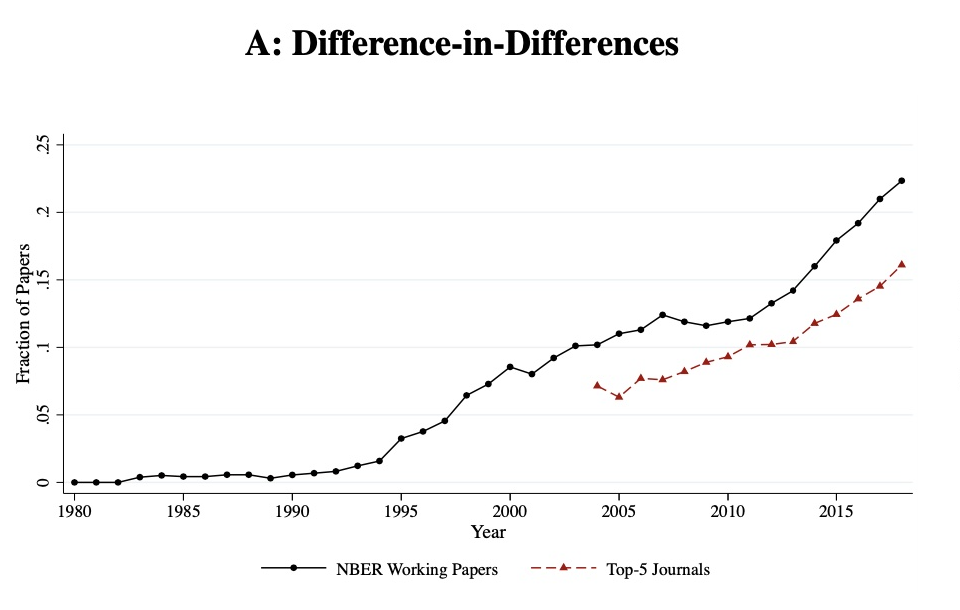
\includegraphics[scale=0.25]{./lecture_includes/currie_did.png}
	\end{figure}

\bigskip

\footnotesize

With some exception (e.g., Heckman, Ichimura and Todd 1997; Abadie 2005; Bertrand, Duflo and Mullainthan 2004), econometricians had not given it much notice

\end{frame}

\begin{frame}{Beaver dam and diff-in-diff credibility crisis}
  \begin{columns}
    \begin{column}{0.5\textwidth}
      \begin{itemize}
\item Differential timing literature is like a stick that struck a beaver's dam
\item Stick made a hole causing a leak
\item Gradually that hole got larger and the leak got bigger
\item Eventually the dam collapsed 
\item That's now
      \end{itemize}
    \end{column}
    \begin{column}{0.5\textwidth}
      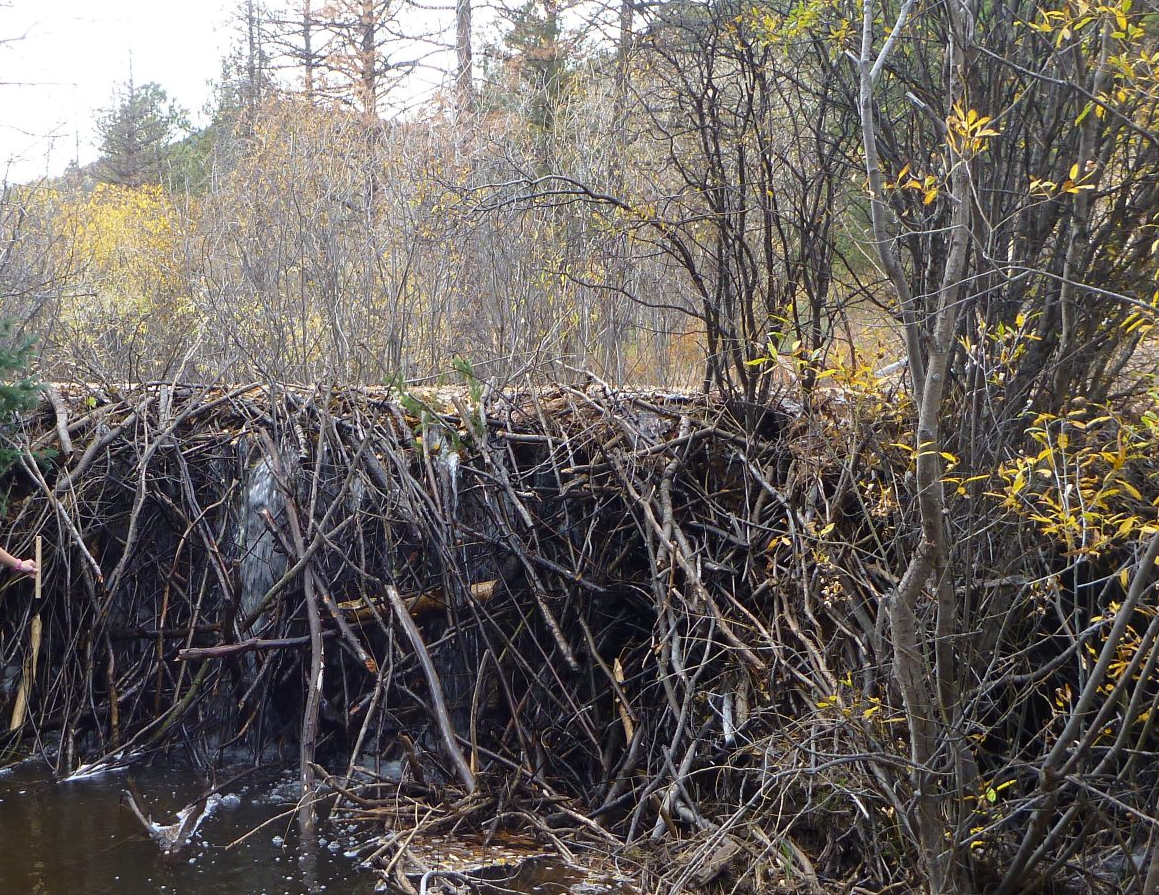
\includegraphics[scale=0.25]{./lecture_includes/beaverdam}
    \end{column}
  \end{columns}
\end{frame}


\begin{frame}{Difference-in-differences credibility crisis}

\begin{itemize}
\item Beginning in 2016-2017, several grad students and assistant professors found critical pathologies with standard TWFE specifications and developed solutions  
\item Many simultaneous discoveries, some redundancies, and \textbf{sudden} awareness of the issues started happening around 2017, eventually became a massive thing
\item Extreme meteoric rise, unusual for econometrics
\end{itemize}

\end{frame}



\begin{frame}{Borusyak et al}
  \begin{columns}
    \begin{column}{0.5\textwidth}
      \begin{itemize}
\item Starts it all; written as grad students at Harvard
\item Goes through many revisions, posted as working paper
\item Returned to a few years ago with a third coauthor, Jahn Spiess, just accepted this week at Restud
      \end{itemize}
    \end{column}
    \begin{column}{0.5\textwidth}
      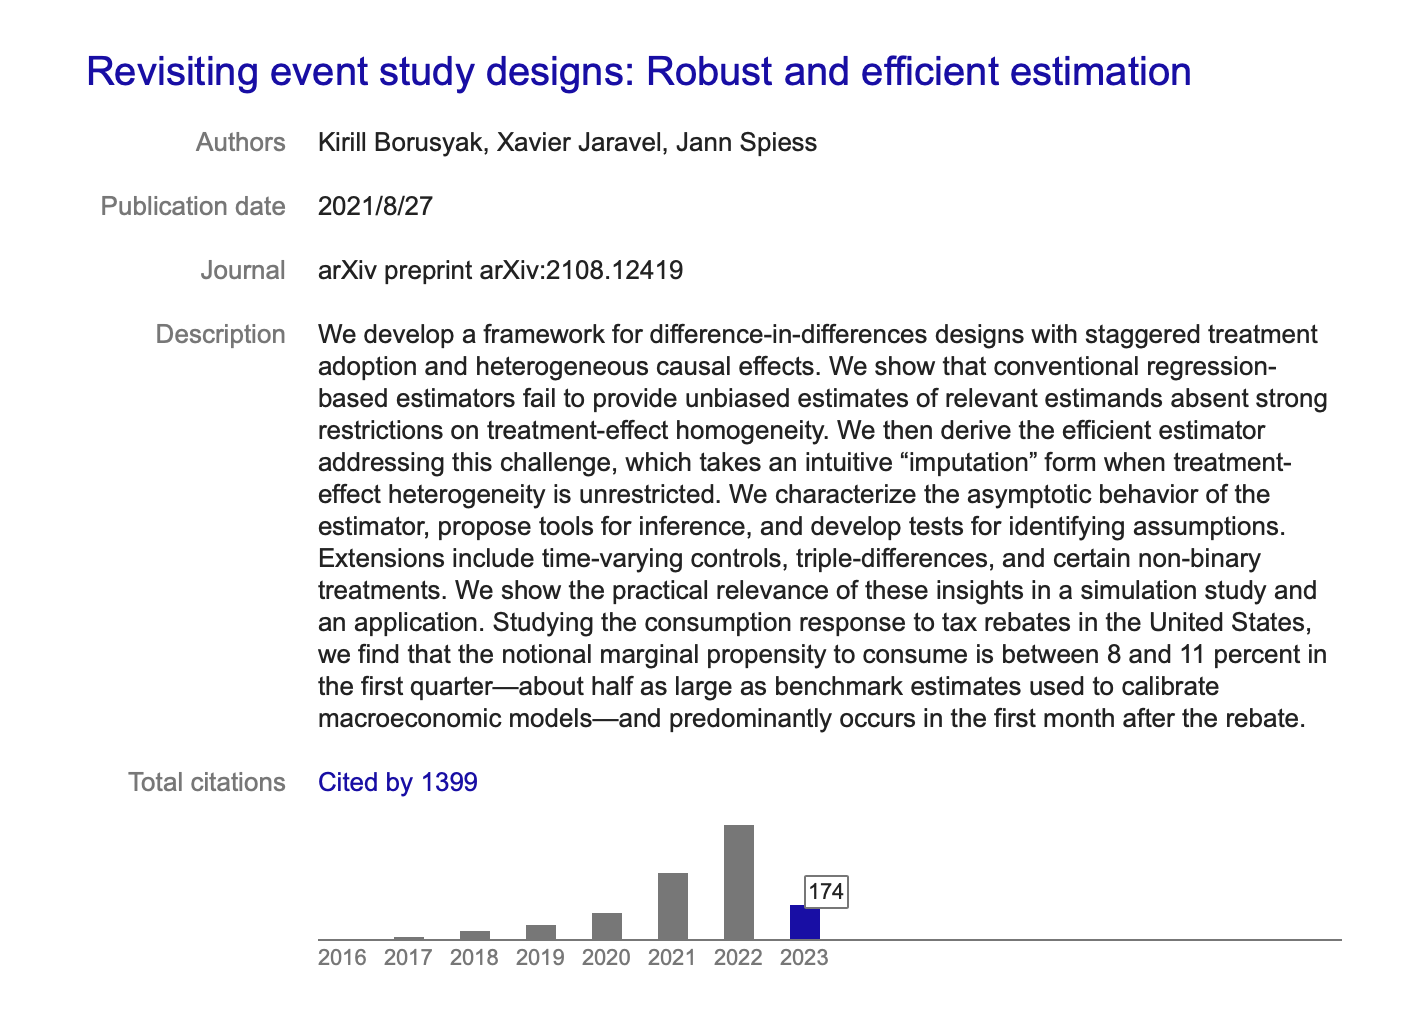
\includegraphics[scale=0.25]{./lecture_includes/kirill_cites}
    \end{column}
  \end{columns}
\end{frame}


\begin{frame}{``dCdH''}
  \begin{columns}
    \begin{column}{0.5\textwidth}
      \begin{itemize}
\item First major hit (in AER), may have been in working paper in 2017 (at least 2018)
\item Very thorough decomposition of the TWFE pathology, very general solution, included Stata code
\item Very active and talented young team (assistant profs when this was done)
      \end{itemize}
    \end{column}
    \begin{column}{0.5\textwidth}
      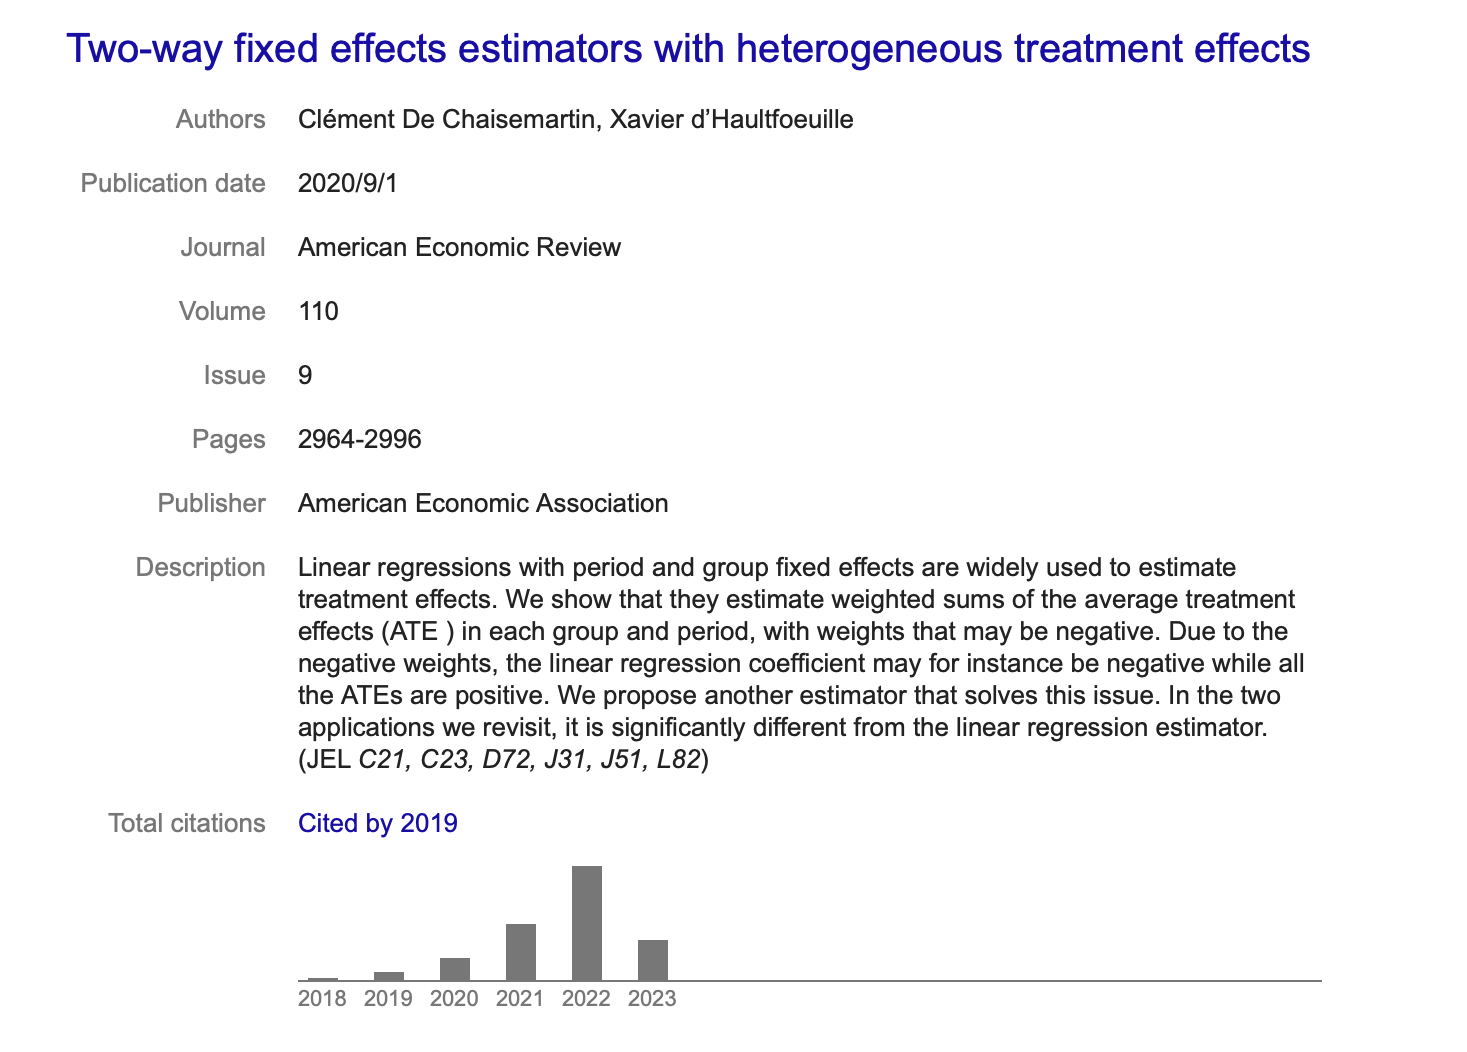
\includegraphics[scale=0.25]{./lecture_includes/dcdh_cites}
    \end{column}
  \end{columns}
\end{frame}

\begin{frame}{Goodman-Bacon}
  \begin{columns}
    \begin{column}{0.5\textwidth}
      \begin{itemize}
\item Arguably the most influential in terms of bringing attention to the problem (but no solution)
\item Begun while grad student at Michigan, published last of the crop
\item Probably Twitter network had a role as he was very active, also not an econometrician
      \end{itemize}
    \end{column}
    \begin{column}{0.5\textwidth}
      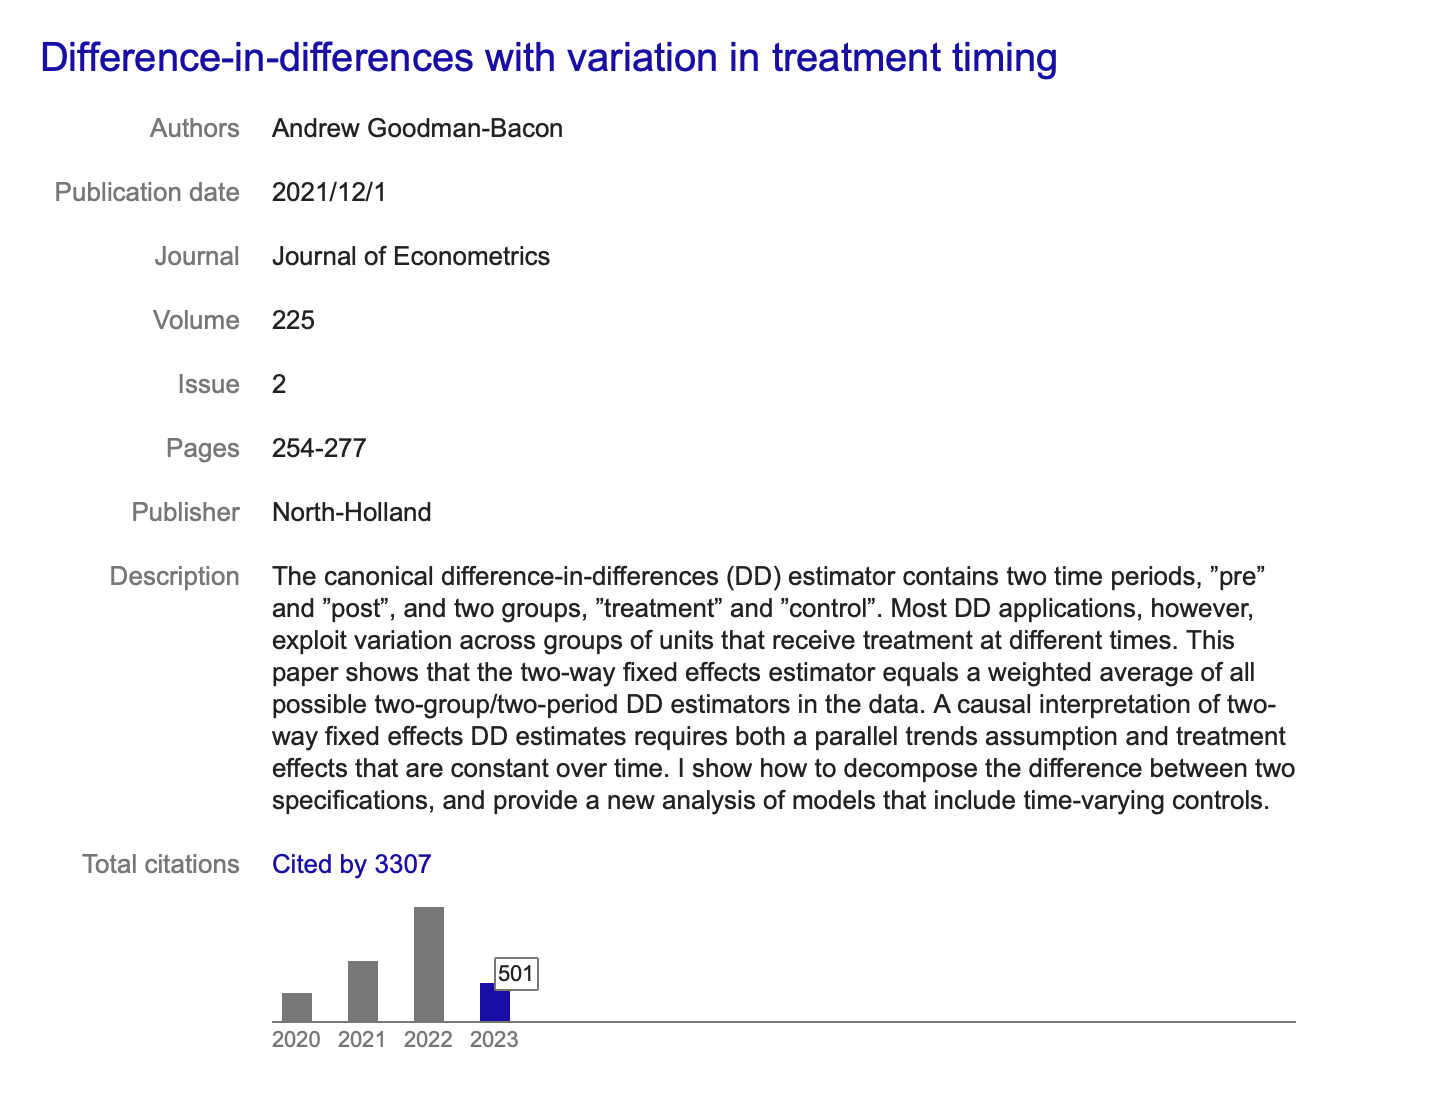
\includegraphics[scale=0.25]{./lecture_includes/andrew_cites}
    \end{column}
  \end{columns}
\end{frame}


\begin{frame}{``CS''}
  \begin{columns}
    \begin{column}{0.5\textwidth}
      \begin{itemize}
\item Second published solution to the problem, written while assistant professors at Vanderbilt and Ole Miss, 
\item Pedro is a UC3M alum (2015 grad) and Brantly is a Vanderbilt grad
\item Both are now coauthors with Andrew Goodman-Bacon
\item Introduced new terms like group-time ATT, released very tight R code (``did'')
      \end{itemize}
    \end{column}
    \begin{column}{0.5\textwidth}
      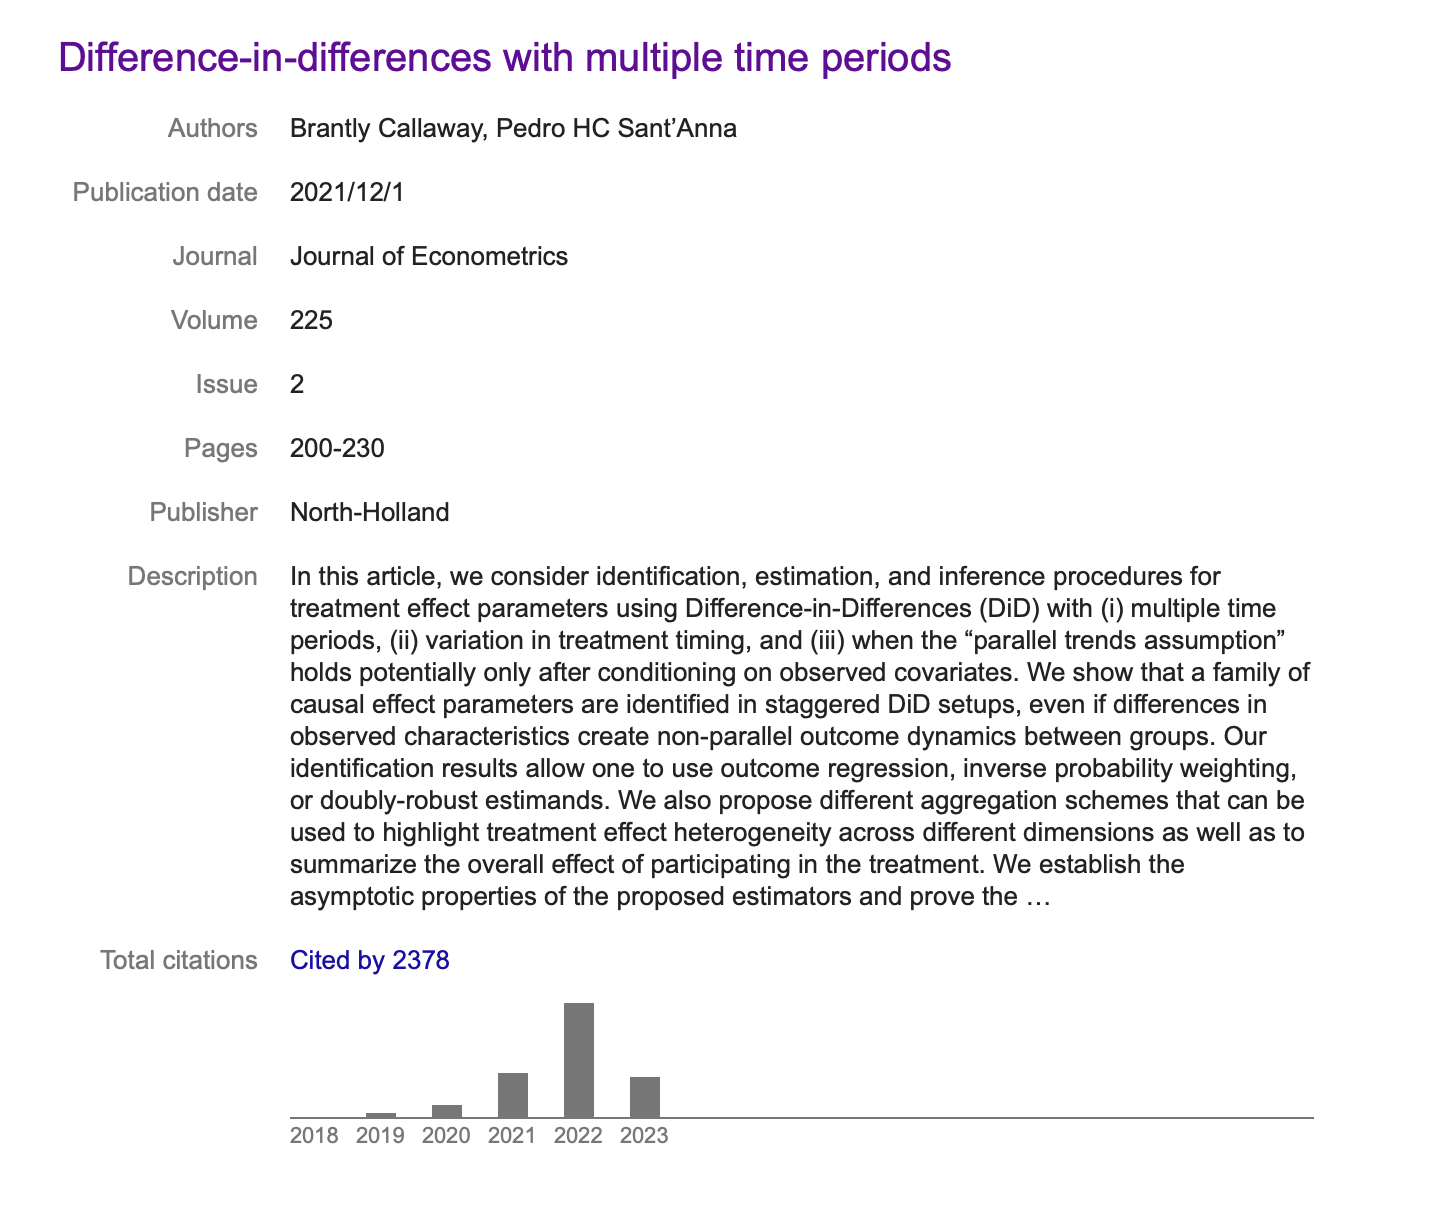
\includegraphics[scale=0.25]{./lecture_includes/pedro_cites}
    \end{column}
  \end{columns}
\end{frame}



\begin{frame}{``SA''}
  \begin{columns}
    \begin{column}{0.5\textwidth}
      \begin{itemize}
\item Third published solution to the problem, very similar to CS
\item Focus was on decomposing the event study
\item Written while grad students at MIT but Sophie Sun is now an assistant professor at CEMFI!
      \end{itemize}
    \end{column}
    \begin{column}{0.5\textwidth}
      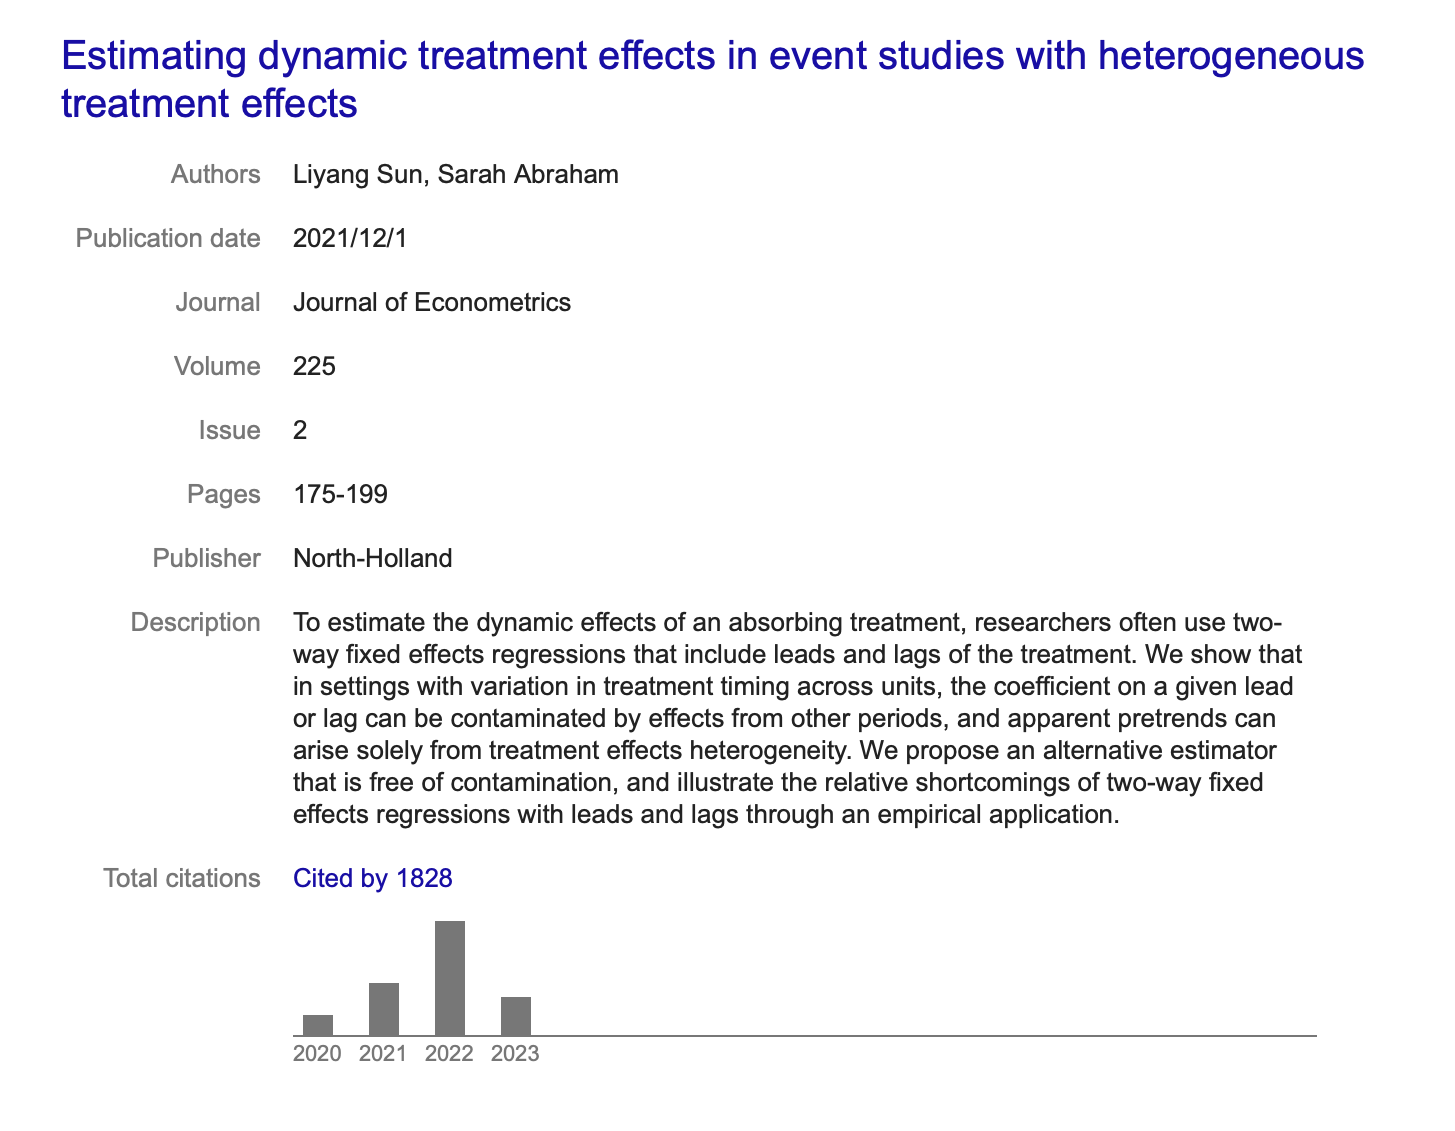
\includegraphics[scale=0.25]{./lecture_includes/sun_cites}
    \end{column}
  \end{columns}
\end{frame}

\begin{frame}{There's even more and more coming}

\begin{itemize}
\item Gardner, Wooldridge, John Roth, and on and on
\item Too many people to name at this point
\item Given the large cites, we are likely to keep seeing more on this
\item Probably shifting applied practice for the better but there are some growing pains
\end{itemize}

\end{frame}


\subsection{TWFE Pathologies}





\begin{frame}{Diff-in-diff and OLS}
$$Y_{ist} = \alpha_0 + \alpha_1 Treat_{is} + \alpha_2 Post_{t} + \textcolor{blue}{\delta} (Treat_{is} \times Post_t) + \varepsilon_{ist} $$

\bigskip

$$\widehat{\textcolor{blue}{\delta}} = \bigg ( \overline{y}_k^{post(k)} - \overline{y}_k^{pre(k)} \bigg ) - \bigg ( \overline{y}_U^{post(k)} - \overline{y}_U^{pre(k)} \bigg ) $$

\begin{itemize}
\item Orley claims that the TWFE estimator of $\delta$ and the ``four averages and three subtractions'' are the same thing numerically
\item Without covariates, they are numerically \emph{identical}
\item But this model requires only one treated unit (i.e., Post is undefined for more than one treatment group)
\end{itemize}

\end{frame}



\begin{frame}{Discussion of estimate}


$$Y_{ist} = \beta_0 + \delta D_{ist} + \tau_t + \sigma_s + \varepsilon_{ist}$$


\begin{itemize}
\item The above is the workhorse model with differential timing -- twoway fixed effects (year and panel unit fixed effects additive in the model)
\item If you estimate this model under differential timing of the treatment, what parameter then does $\widehat{\delta}$ correspond to?
\item Answer: It also corresponds to the previous ``four averages and three subtractions'' -- but it's numerous of them, not just one

\end{itemize}

\end{frame}



\begin{frame}{Decomposition Preview}


\begin{itemize}
\item Andrew Goodman-Bacon decomposed $\widehat{\delta}$ and showed it is numerically identical to a weighted average of all ``four averages and three subtractions''
\item But, even before we get to causality there are unusual features
\item TWFE model assigns its own weights which are a function of the size of a ``group'' and the variance of group treatment dummies
\end{itemize}

\end{frame}



\begin{frame}{$K^2$ distinct DDs}

Let's look at 3 timing groups (a, b and c) and one untreated group (U).  With 3 timing groups, there are 9 2x2 DDs.  Here they are:


\begin{center}
\begin{tabular}{c|c|c}
\multicolumn{1}{l}{} &
\multicolumn{1}{l}{} &
\multicolumn{1}{l}{} \\
\midrule
a to b & b to a & c to a \\
a to c & b to c & c to b \\
a to U & b to U & c to U \\
\midrule
\end{tabular}
\end{center}

\bigskip

Let's return to a simpler example with only two groups -- a $k$ group treated at $t_k^*$ and an $l$ treated at $t_l^*$ plus an never-treated group called the $U$ untreated group
\end{frame} 


\begin{frame}{Terms and notation}

\begin{itemize}
\item Let there be two treatment groups (k,l) and one untreated group (U)
\item k,l define the groups based on when they receive treatment (differently in time) with k receiving it earlier than l
\item Denote $\overline{D}_k$ as the share of time each group spends in treatment status
\item Denote $\widehat{\delta}_{jb}^{2x2}$ as the canonical $2\times 2$ DD estimator for groups $j$ and b where $j$ is the treatment group and $b$ is the comparison group
\end{itemize}

\end{frame}


\imageframe{./lecture_includes/bacon_goodman_2.png}



\begin{frame}[plain]
$$\widehat{\delta}^{2x2}_{kU} = \bigg ( \overline{y}_k^{post(k)} - \overline{y}_k^{pre(k)} \bigg ) - \bigg ( \overline{y}_U^{post(k)} - \overline{y}_U^{pre(k)} \bigg ) $$
	\begin{figure}
	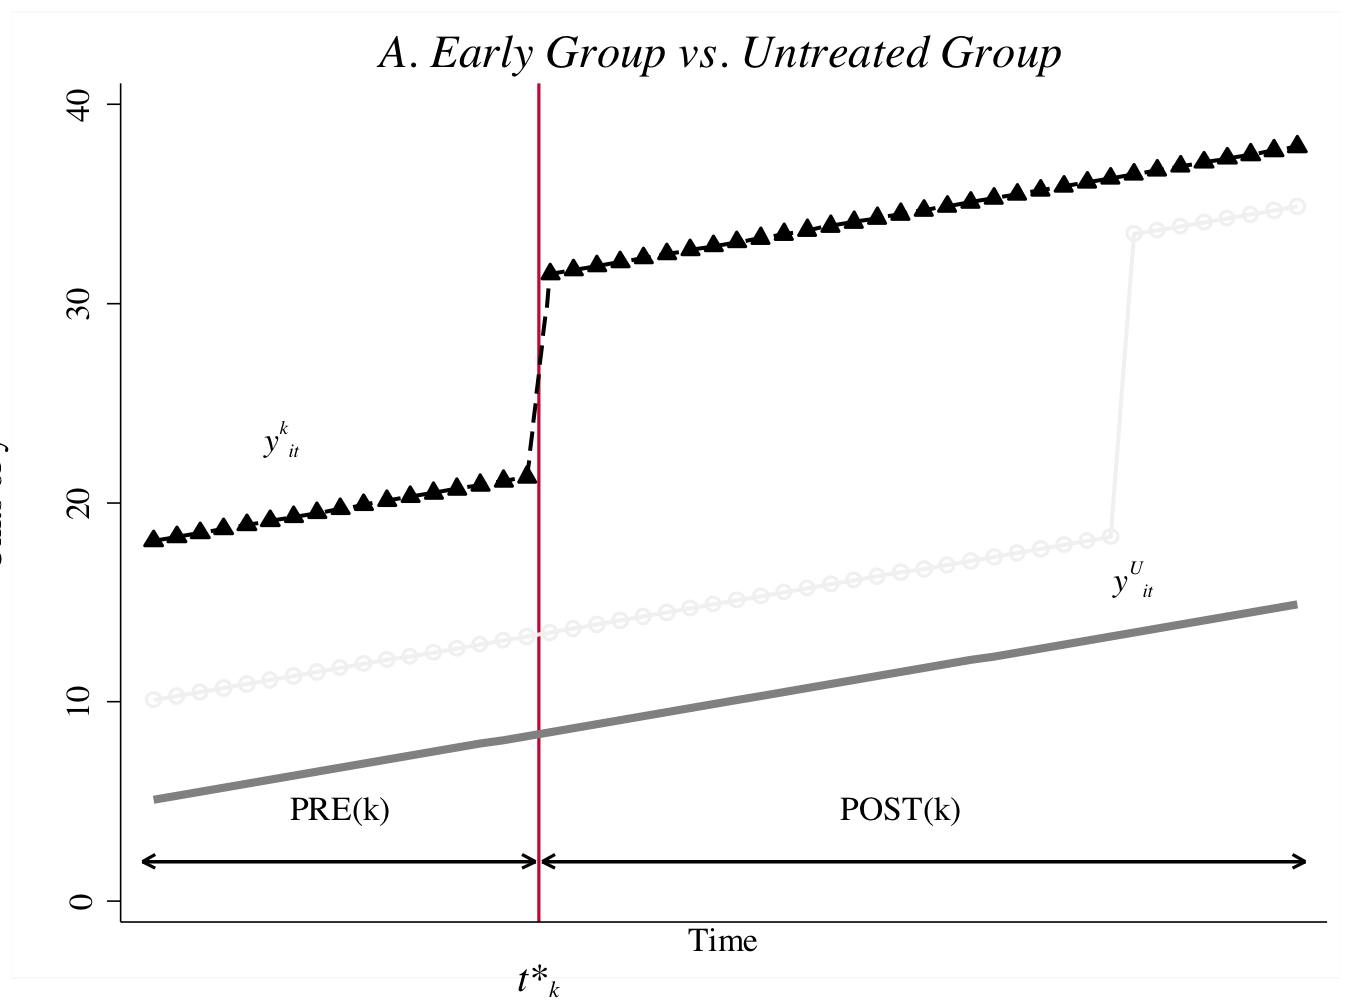
\includegraphics[scale=0.45]{./lecture_includes/bacon_goodman_3.png}
	\end{figure}

\end{frame}

\begin{frame}[plain]
$$\widehat{\delta}^{2x2}_{lU} = \bigg ( \overline{y}_l^{post(l)} - \overline{y}_l^{pre(l)} \bigg ) - \bigg ( \overline{y}_U^{post(l)} - \overline{y}_U^{pre(l)} \bigg ) $$
	\begin{figure}
	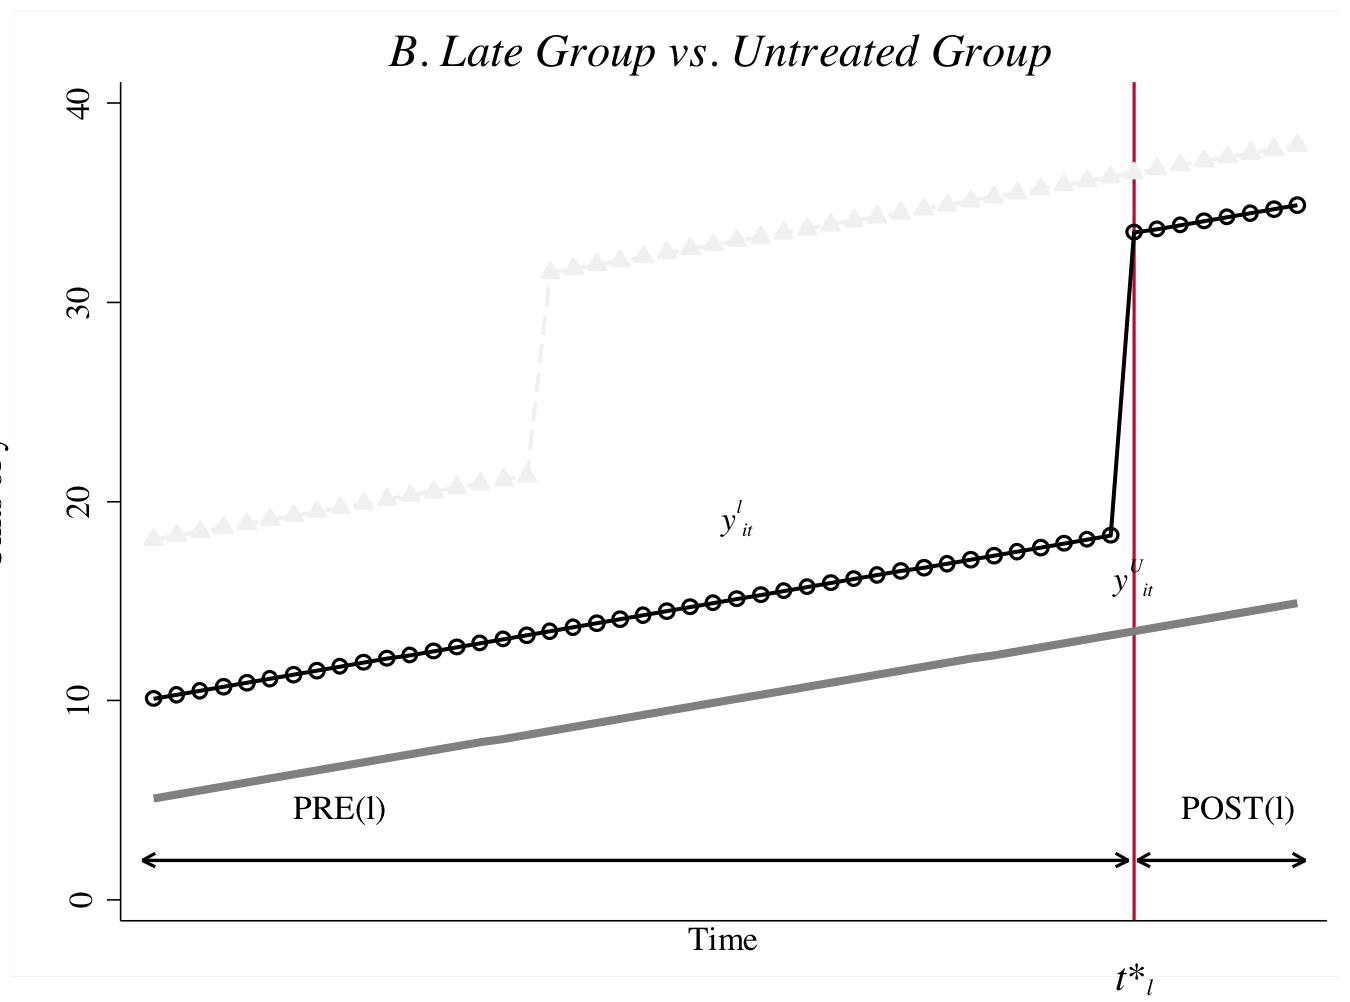
\includegraphics[scale=0.45]{./lecture_includes/bacon_goodman_4.png}
	\end{figure}

\end{frame}


\begin{frame}[plain]

$$\delta_{kl}^{2x2,k} = \bigg ( \overline{y}_k^{MID(k,l)} - \overline{y}_k^{Pre(k,l)} \bigg ) - \bigg ( \overline{y}_l^{MID(k,l)} - \overline{y}_l^{PRE(k,l)} \bigg ) $$

	\begin{figure}
	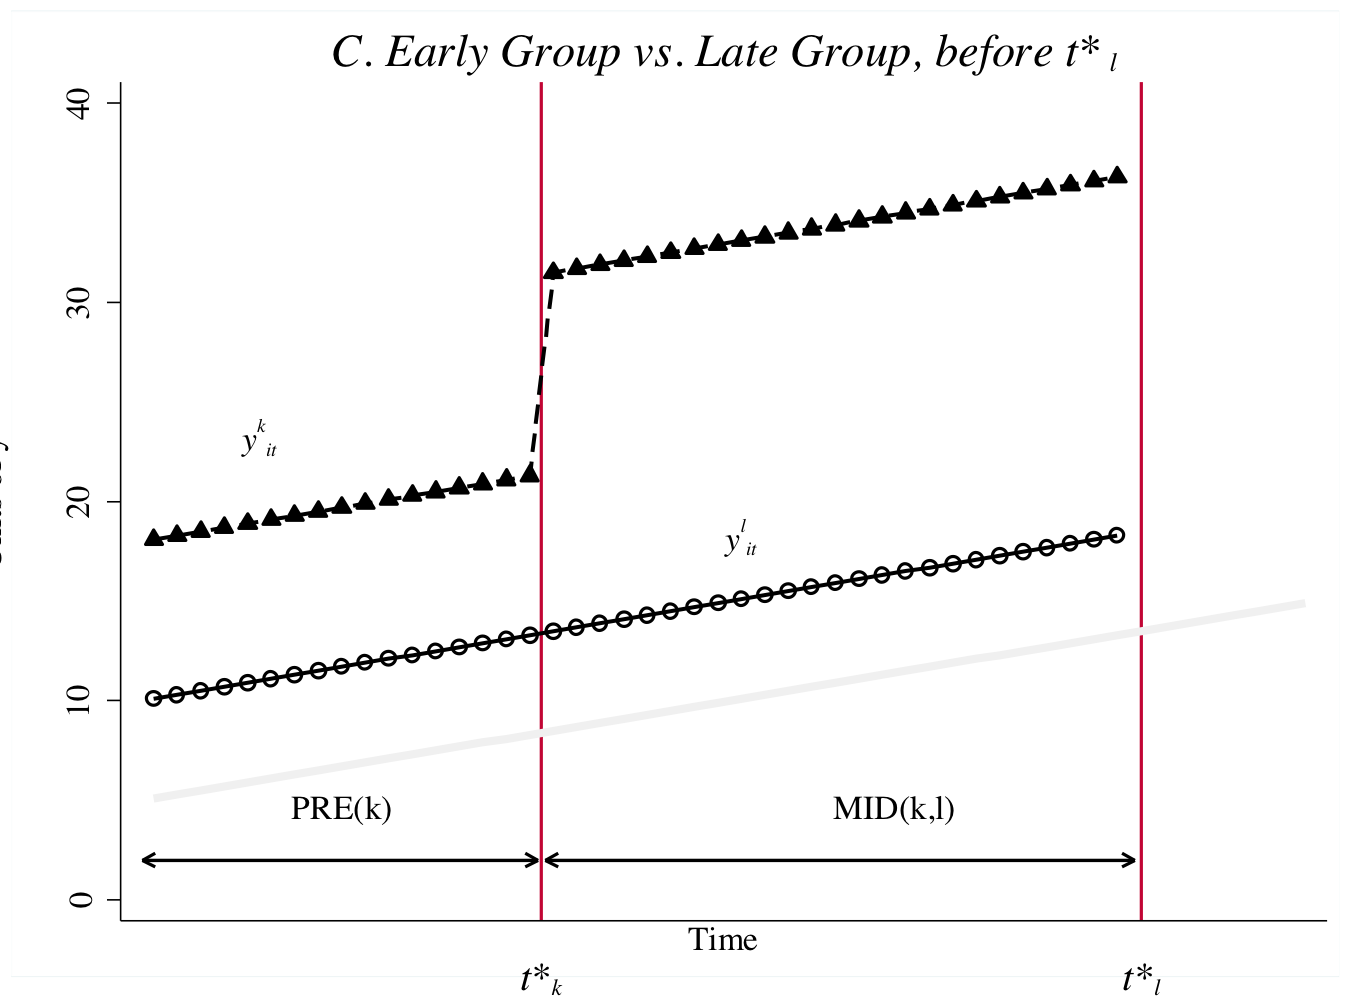
\includegraphics[scale=0.45]{./lecture_includes/bacon_goodman_6.png}
	\end{figure}

\end{frame}

\begin{frame}[plain]
$$\delta_{lk}^{2x2,l} = \bigg ( \overline{y}_l^{POST(k,l)} - \overline{y}_l^{MID(k,l)} \bigg ) - \bigg ( \overline{y}_k^{POST(k,l)} - \overline{y}_k^{MID(k,l)} \bigg ) $$

	\begin{figure}
	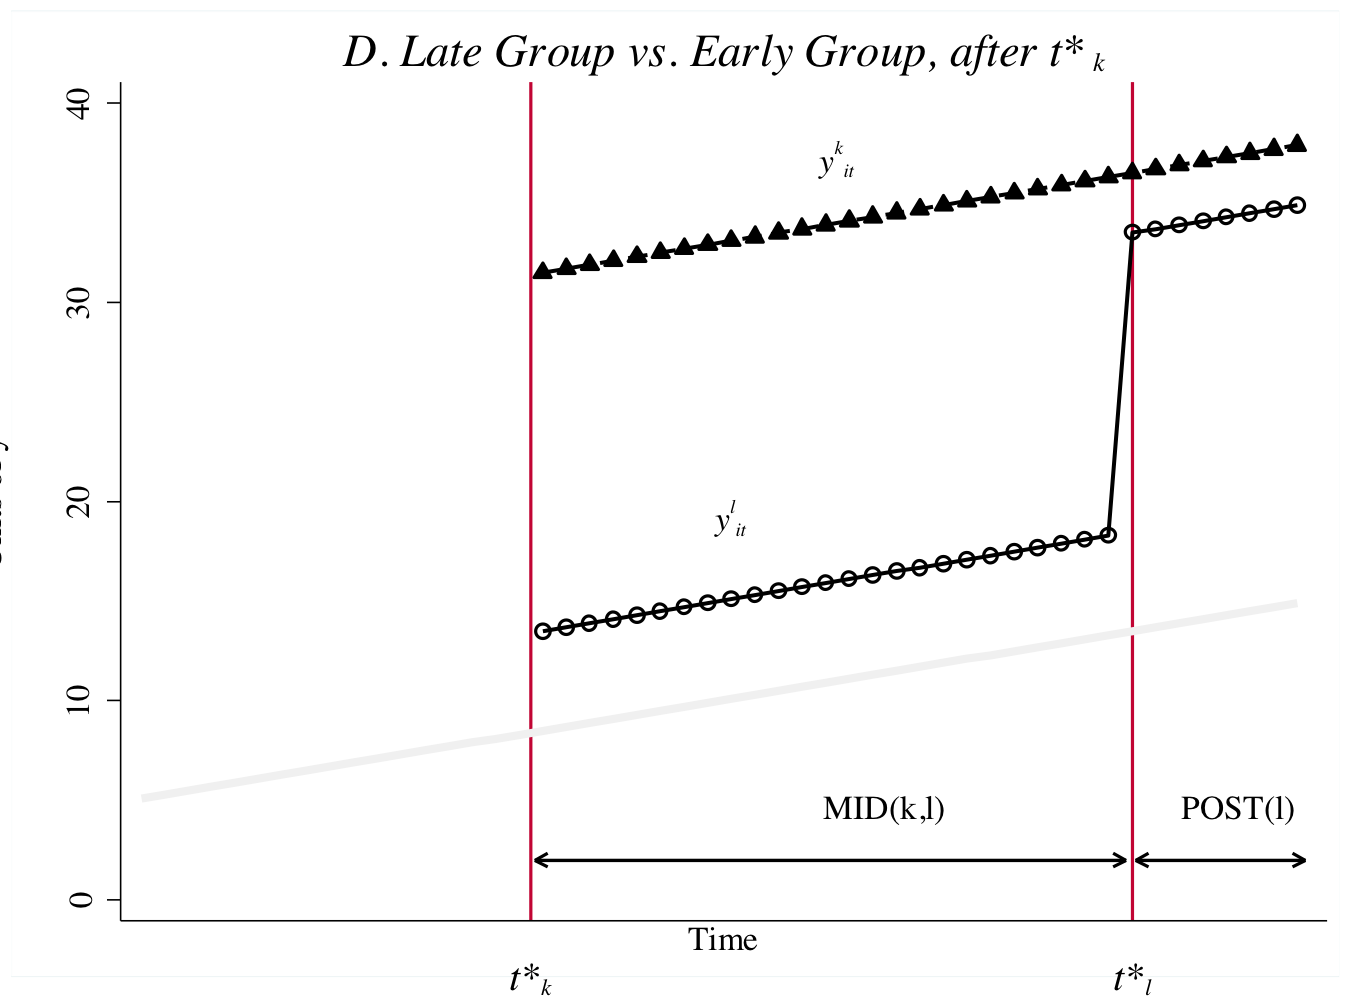
\includegraphics[scale=0.4]{./lecture_includes/bacon_goodman_7.png}
	\end{figure}

\end{frame}


	

\begin{frame}{Bacon decomposition}

$$Y_{ist} = \beta_0 + \delta D_{ist} + \tau_t + \sigma_s + \varepsilon_{ist}$$


TWFE estimate of $\widehat{\delta}$ is equal to a weighted average over all group 2x2 (of which there are 4 in this example)
\begin{eqnarray*}	
\widehat{\delta}^{TWFE} = \sum_{k \neq U} s_{kU}\widehat{\delta}_{kU}^{2x2} + \sum_{k \neq U} \sum_{l>k} s_{kl}  \bigg [ \mu_{kl}\widehat{\delta}_{kl}^{2x2,k} + (1-\mu_{kl}) \widehat{\delta}_{lk}^{2x2,l} \bigg]
\end{eqnarray*}where that first 2x2 combines the k compared to U and the l to U (combined to make the equation shorter)

\end{frame}
	


\begin{frame}{Third, the Weights}

 \begin{eqnarray*} s_{ku} &=& \frac{ n_k n_u \overline{D}_k (1- \overline{D}_k ) }{ \widehat{Var} ( \tilde{D}_{it} )} \\
s_{kl} &=& \frac{ n_k n_l (\overline{D}_k - \overline{D}_{l} ) ( 1- ( \overline{D}_k - \overline{D}_{l} )) }{\widehat{Var}(\tilde{D}_{it})} \\
\mu_{kl} &=& \frac{1 - \overline{D}_k }{1 - ( \overline{D}_k - \overline{D}_{l} )}
\end{eqnarray*}where $n$ refer to sample sizes, $\overline{D}_k (1- \overline{D}_k )$ $(\overline{D}_k - \overline{D}_{l} ) ( 1- ( \overline{D}_k - \overline{D}_{l} ))$ expressions refer to variance of treatment, and the final equation is the same for two timing groups.

\end{frame}

\begin{frame}{Weights discussion}

\begin{itemize}
\item Two things to note:
	\begin{itemize}
	\item More units in a group, the bigger its 2x2 weight is
	\item Group treatment variance weights up or down a group's 2x2
	\end{itemize}
\item Think about what causes the treatment variance to be as big as possible. Let's think about the $s_{ku}$ weights.
	\begin{itemize}
	\item $\overline{D}=0.1$. Then $0.1 \times 0.9 = 0.09$
	\item $\overline{D}=0.4$. Then $0.4 \times 0.6 =0.24$
	\item $\overline{D}=0.5$. Then $0.5 \times 0.5 = 0.25$
	\item $\overline{D}=0.6$. Then $0.6 \times 0.4 = 0.24$
	\end{itemize}
\item This means the weight on treatment variance is maximized for \emph{groups treated in middle of the panel}
\end{itemize}
\end{frame}

\begin{frame}{More weights discussion}

\begin{itemize}
\item But what about the ``treated on treated'' weights (i.e., $\overline{D}_k - \overline{D}_{l} $)  
\item Same principle as before - when the difference between treatment variance is close to 0.5, those 2x2s are given the greatest weight
\item For instance, say $t^*_k=0.15$ and $t^*_l=0.67$. Then $\overline{D}_k - \overline{D}_{l} = 0.52$.  And thus $0.52 \times 0.48 = 0.2496$.
\end{itemize}

\end{frame}


\begin{frame}{Summarizing TWFE centralities}

\begin{itemize}
\item Groups in the middle of the panel weight up their respective 2x2s via the variance weighting
\item Decomposition highlights the strange role of panel length when using TWFE
\item Different choices about panel length change both the 2x2 and the weights based on variance of treatment
\end{itemize}

\end{frame}




\begin{frame}{Back to TWFE}


$$Y_{ist} = \beta_0 + \delta D_{ist} + \tau_t + \sigma_s + \varepsilon_{ist}$$


\begin{itemize}

\item So we saw that with differential timing, $\widehat{\delta}$ is a weighted average over all ``four averages and three subtractions'' but is that good or bad?
\item Bacon's decomposition doesn't say anything about bias (yet)
\item We will need to replace realized outcomes with potential outcomes in order to understand the nature of bias and causal identification 

\end{itemize}

\end{frame}

\begin{frame}{Back to TWFE}


$$Y_{ist} = \beta_0 + \delta D_{ist} + \tau_t + \sigma_s + \varepsilon_{ist}$$


\begin{itemize}

\item Bacon shows that TWFE estimate of $\delta$ needs two assumptions for unbiasedness:
	\begin{enumerate}
	\item variance weighted parallel trends are zero and 
	\item no dynamic treatment effects (not the case with 2x2)
	\end{enumerate}
\item Under those assumptions, TWFE estimator estimates the variance weighted ATT as a weighted average of all possible ATTs (not just weighted average of DiDs)

\end{itemize}

\end{frame}


\begin{frame}{Moving from 2x2s to causal effects and bias terms}

Let's start breaking down these estimators into their corresponding estimation objects expressed in causal effects and biases


\begin{eqnarray*}
\widehat{\delta}^{2x2}_{kU} &=& ATT_k{Post} + \Delta Y^0_k(Post(k),Pre(k)) - \Delta Y^0_U(Post(k),Pre) \\
\widehat{\delta}^{2x2}_{kl} &=& ATT_k(MID) + \Delta Y^0_k(MID,Pre) - \Delta Y^0_l(MID, Pre)
\end{eqnarray*}These look the same because you're always comparing the treated unit with an untreated unit (though in the second case it's just that they haven't been treated \emph{yet}). 

\end{frame}

\begin{frame}{The dangerous 2x2}

But what about the 2x2 that compared the late groups to the already-treated earlier groups? With a lot of substitutions we get:

\begin{eqnarray*}
\widehat{\delta}^{2x2}_{lk} &=& ATT_{l,Post(l)} + \underbrace{\Delta Y^0_l(Post(l),MID) - \Delta Y^0_k ( Post(l), MID)}_{\mathclap{\text{Parallel trends bias}}} \\
&& - \underbrace{(ATT_k(Post) - ATT_k(Mid))}_{\mathclap{\text{Heterogeneity bias!}}}
\end{eqnarray*}

\bigskip

Remember earlier when I made the distinction between true and counterfeit diff-in-diff?  


\end{frame}

\begin{frame}{Substitute all this stuff into the decomposition formula}

\begin{eqnarray*}	
\widehat{\delta}^{TWFE} = \sum_{k \neq U} s_{kU}\widehat{\delta}_{kU}^{2x2} + \sum_{k \neq U} \sum_{l>k} s_{kl}  \bigg [ \mu_{kl}\widehat{\delta}_{kl}^{2x2,k} + (1-\mu_{kl}) \widehat{\delta}_{kl}^{2x2,l} \bigg]
\end{eqnarray*}where we will make these substitutions\begin{eqnarray*}
\widehat{\delta}_{kU}^{2x2} &=& ATT_k(Post) + \Delta Y_l^0(Post,Pre) - \Delta Y_U^0(Post, Pre) \\
\widehat{\delta}_{kl}^{2x2,k} &=& ATT_k(Mid) + \Delta Y_l^0(Mid,Pre) - \Delta Y_l^0(Mid, Pre) \\
\widehat{\delta}^{2x2,l}_{lk} &=& ATT_{l}Post(l) + \Delta Y^0_l(Post(l),MID) - \Delta Y^0_k ( Post(l), MID) \\
&&- (ATT_k(Post) - ATT_k(Mid))
\end{eqnarray*}Notice all those potential sources of biases! 

\end{frame}


\begin{frame}{Potential Outcome Notation}

\begin{eqnarray*}
p\text{ }lim\text{ } \widehat{\delta}^{TWFE}_{n\to\infty} &=& VWATT + VWPT - \Delta ATT
\end{eqnarray*}

\begin{itemize}
\item Notice the number of assumptions needed \emph{even} to estimate this very strange weighted ATT (which is a function of how you drew the panel in the first place). 
\item With dynamics, it attenuates the estimate (bias) and can even reverse sign depending on the magnitudes of what is otherwise effects in the sign in a reinforcing direction! 
\item Model can flip signs (does not satisfy a ``no sign flip property'')
\end{itemize}

\end{frame}



\subsection{Simulation}



\begin{frame}{Simulated data}

\begin{itemize}
\item 1000 firms, 40 states, 25 firms per states, 1980 to 2009 or 30 years, 30,000 observations, four groups

\item I'll impose ``unit level parallel trends'', which is much stronger than we need (we only need average parallel trends)

\item Also no anticipation of treatment effects until treatment occurs but does \emph{not} guarantee homogenous treatment effects

\item Two types of situations: constant versus dynamic treatment effects which can be seen here \url{https://docs.google.com/spreadsheets/d/1dI67eNNE2zrX4KrkoFvej-cKxqHkM8yJdMpD-0uE4q8/edit?usp=sharing}
\end{itemize}
\end{frame}



\begin{frame}{Constant vs Dynamic Treatment Effects}
    \begin{columns}
        \column{0.5\linewidth}
        \centering
        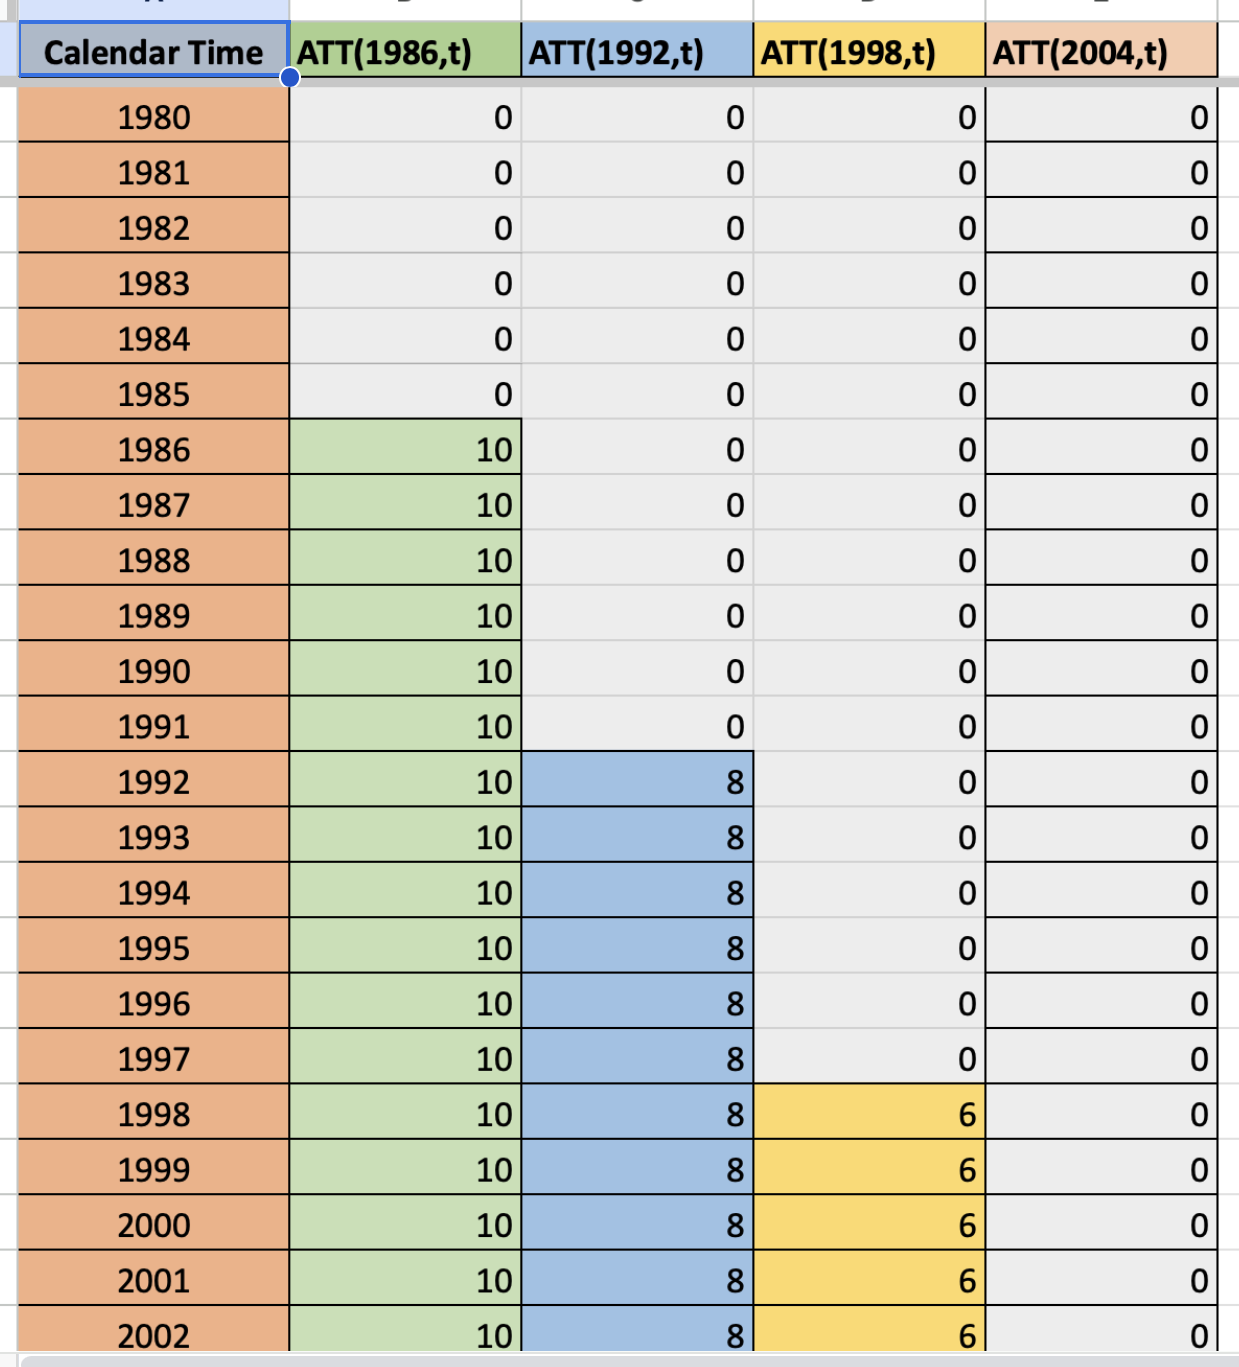
\includegraphics[height=6.5cm, width=5.5cm]{./lecture_includes/constant_te}

        \column{0.5\linewidth}
        \centering
        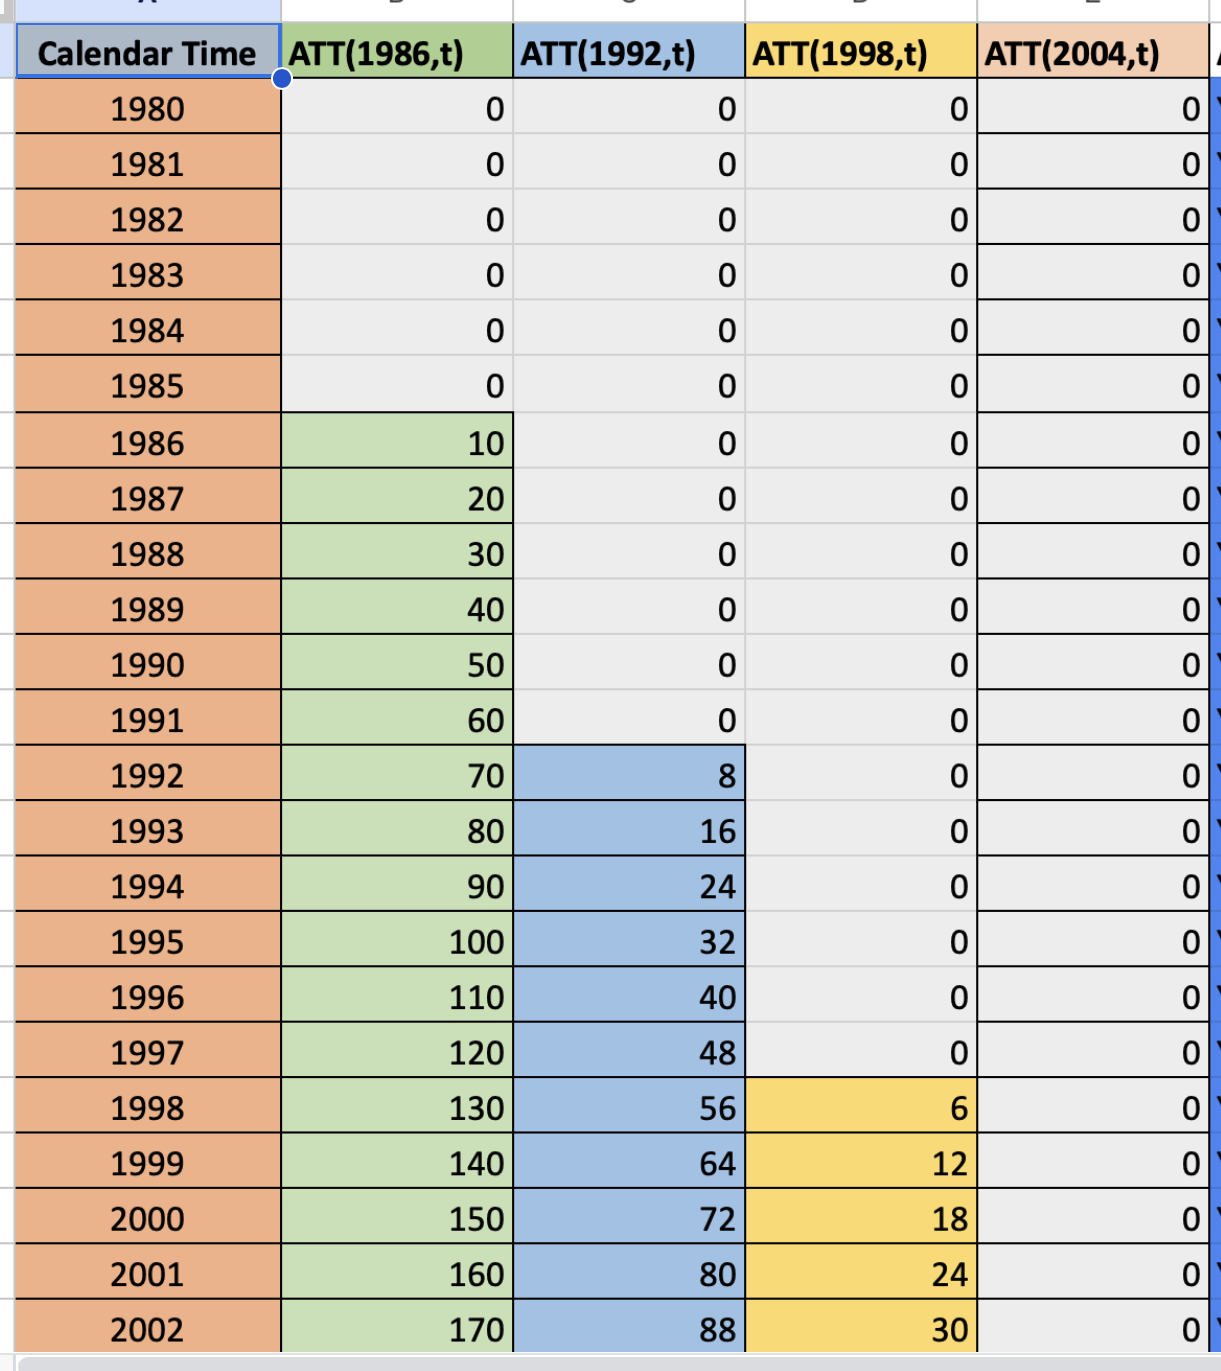
\includegraphics[height=6.5cm, width=5.5cm]{./lecture_includes/dynamic_te}
    \end{columns} 
\end{frame}




\begin{frame}{Group-time ATT}
       \begin{columns}
          \column{0.38\linewidth}
             \centering
             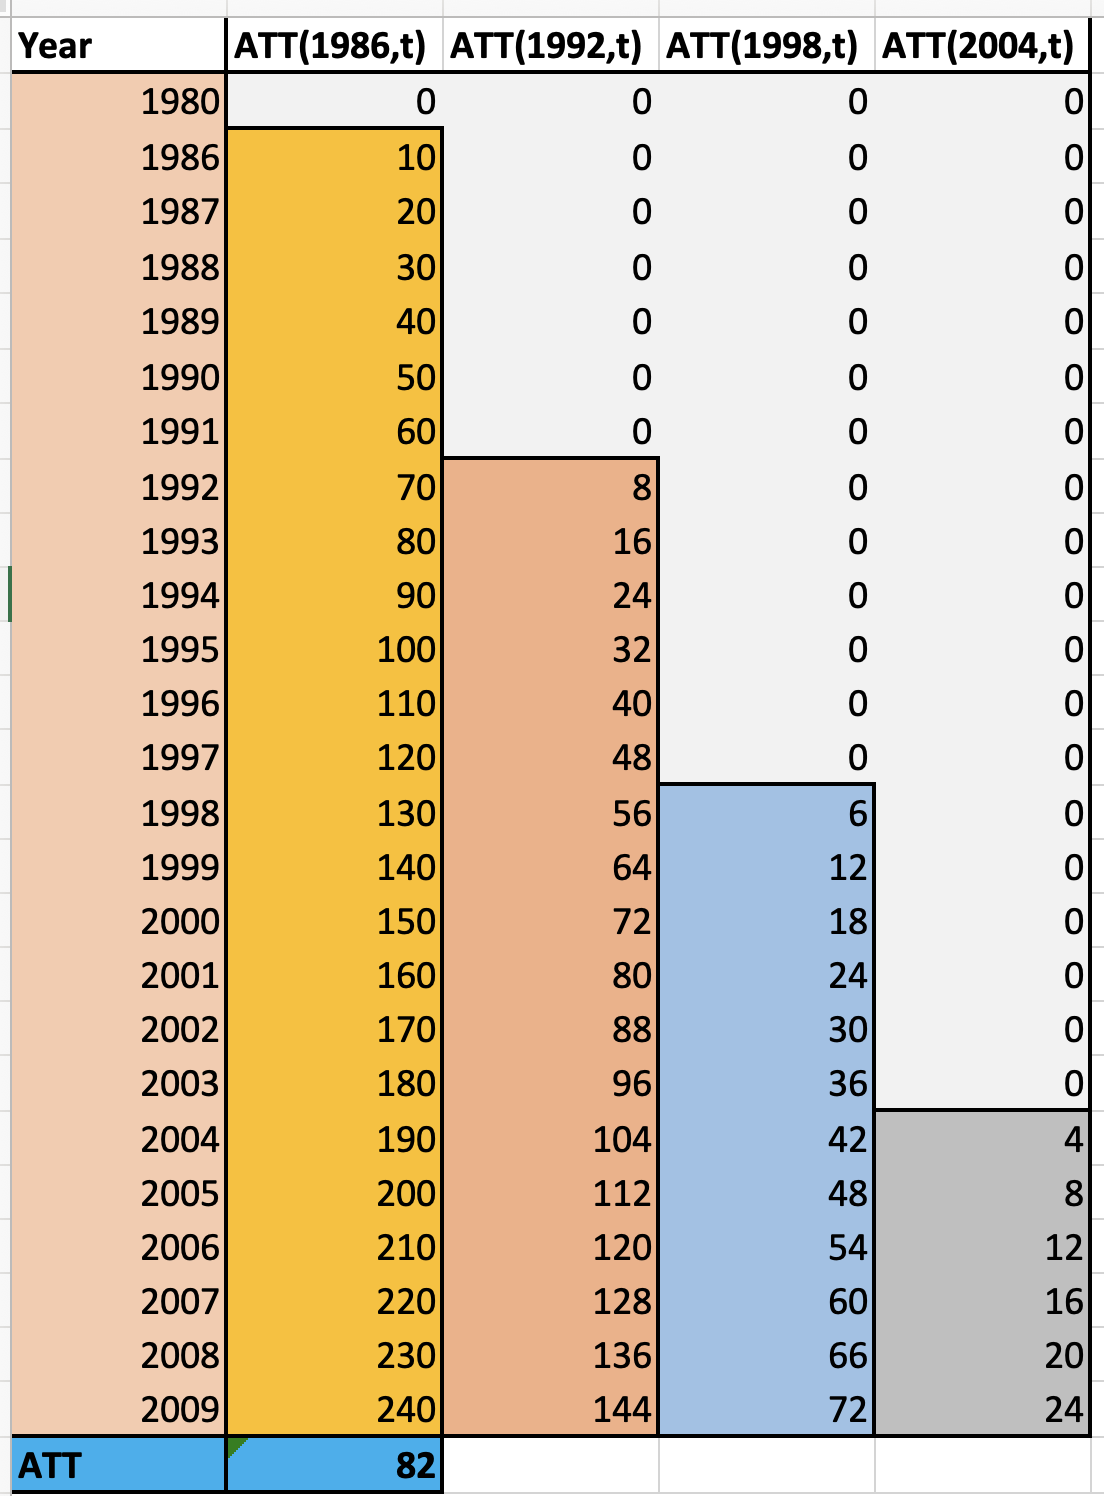
\includegraphics[height=6.5cm, width=5.5cm]{./lecture_includes/baker_attgt}
           \column{0.48\linewidth}
		\begin{itemize}
\item Heterogenous treatment effects across time and across groups
\item Cells are called ``group-time ATT'' (Callaway and Sant'anna 2020) or ``cohort ATT'' (Sun and Abraham 2020)
\item ATT is weighted average of all cells and $+82$ with uniform weights $1/60$
		\end{itemize}
         \end{columns} 
    \end{frame}

\begin{frame}{Estimation}

\bigskip

Estimate the following equation using OLS:

$$Y_{ist} = \alpha_i + \gamma_t +\delta D_{it} + \varepsilon_{ist}$$


\begin{table}[htbp]\centering
\small
\caption{Estimating ATT with different models}
\begin{center}
\begin{tabular}{l*{5}{c}}
\hline
\multicolumn{1}{l}{\textbf{}}&
\multicolumn{1}{c}{\textbf{Truth}}&
\multicolumn{1}{c}{\textbf{(TWFE)}}&
\multicolumn{1}{c}{\textbf{(CS)}}&
\multicolumn{1}{c}{\textbf{(SA)}}&
\multicolumn{1}{c}{\textbf{(BJS)}}\\
\hline
$\widehat{ATT}$  & 82    & -6.69*** &&&\\
\hline
\end{tabular}
\end{center}
\end{table}

The sign flipped.  Why?  Because of \emph{extreme} dynamics (i.e., $- \Delta ATT$)

\end{frame}

\begin{frame}{Bacon decomposition}
\begin{table}[htbp]\centering
\small
\caption{Bacon Decomposition (TWFE $= -6.69$)}
\begin{center}
\begin{tabular}{l*{5}{c}}
\hline
\multicolumn{1}{l}{\textbf{DD Comparison}}&
\multicolumn{1}{l}{\textbf{Weight}}&
\multicolumn{1}{l}{\textbf{Avg DD Est}}\\
\hline
Earlier T vs. Later C  &     0.500   &       51.800 \\
Later T vs. Earlier C   &    0.500    &     -65.180 \\
\midrule
T $=$ Treatment; C$ =$ Comparison \\
$(0.5*51.8) + (0.5*-65.180) = -6.69$ \\
\hline
\end{tabular}
\end{center}
\end{table}

\bigskip

While large weight on the ``late to early 2x2'' is \emph{suggestive} of an issue, these would appear even if we had constant treatment effects

\end{frame}










\section{Robust Diff-in-Diff Estimators}

\subsection{CS}



\begin{frame}{Callaway and Sant'Anna 2020}

CS is a DiD estimator used for estimating and then summarizing smaller ATT parameters under differential timing and conditional parallel trends into more policy relevant ATT parameters (either dynamic or static)


\begin{figure}
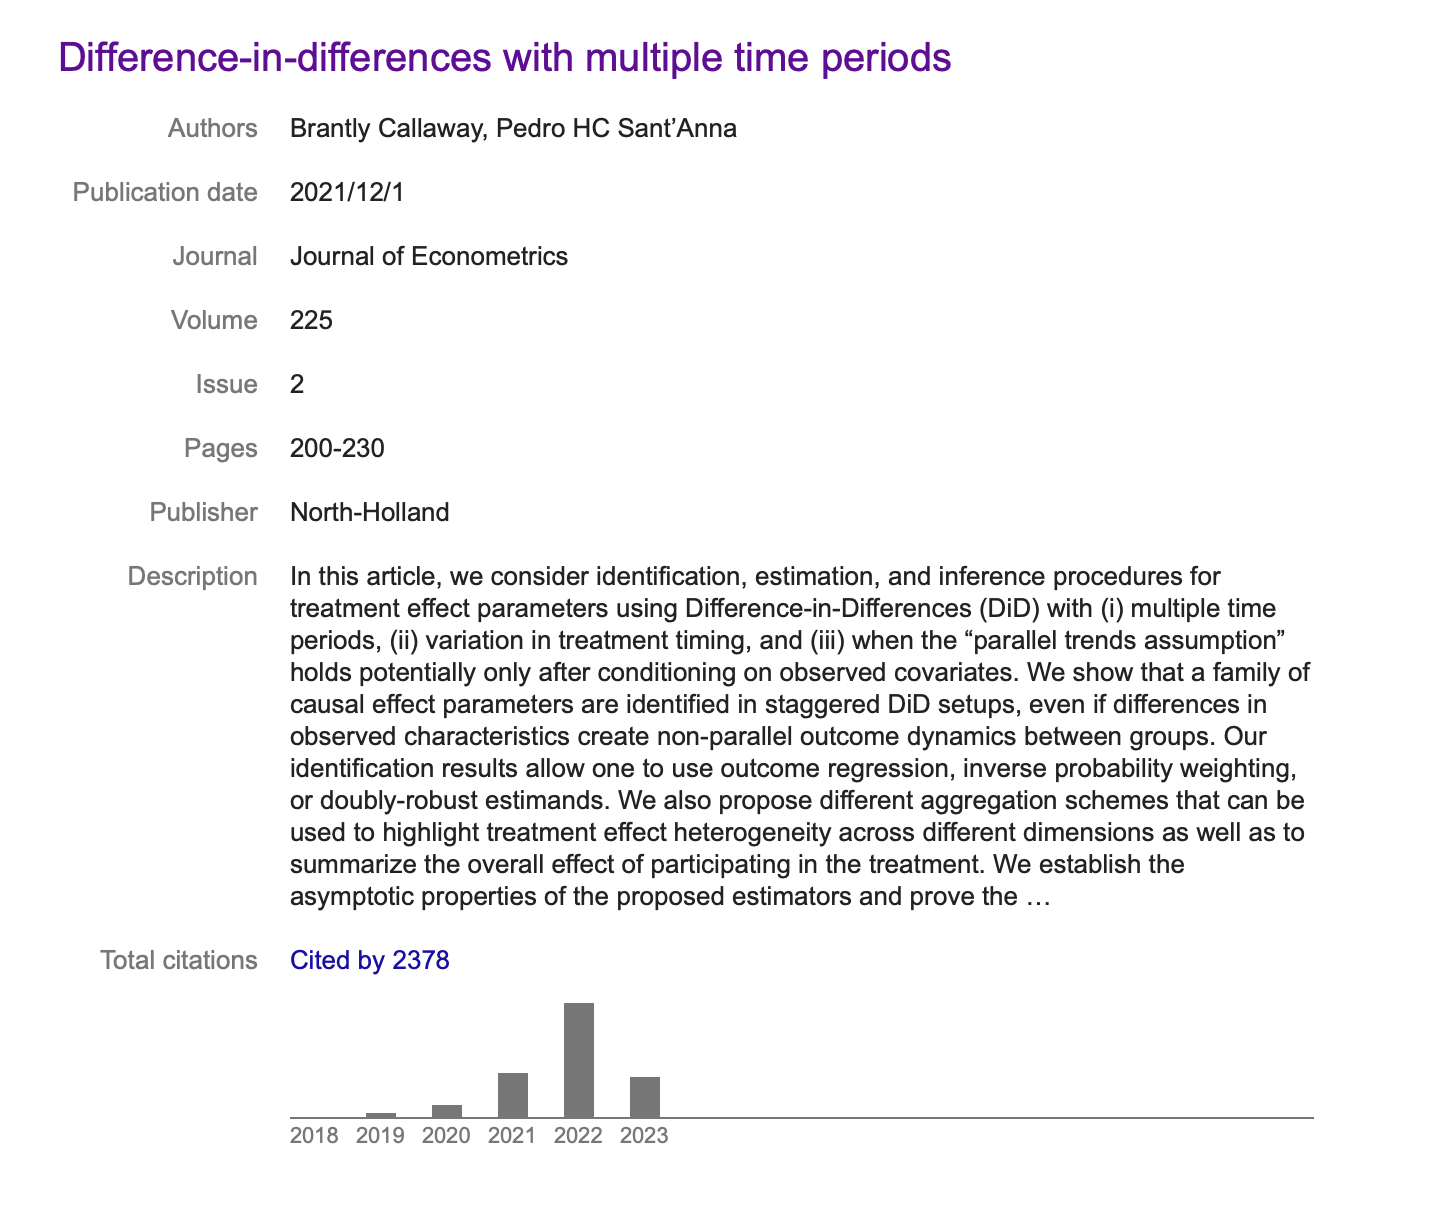
\includegraphics[scale=0.25]{./lecture_includes/pedro_cites}
\end{figure}

\end{frame}


\begin{frame}{When is CS used}

Just some examples of when you'd want to consider it:
\begin{enumerate}
\item When treatment effects differ depending on when it was adopted
\item When treatment effects change over time
\item When shortrun treatment effects are different than longrun effects
\item When treatment effect dynamics differ if people are first treated in a recession relative to expansion years
\end{enumerate}

\bigskip

CS estimates the ATT by identifying smaller causal effects and aggregating them using non-negative weights

\end{frame}






\begin{frame}{Group-time ATT}
       \begin{columns}
          \column{0.38\linewidth}
             \centering
             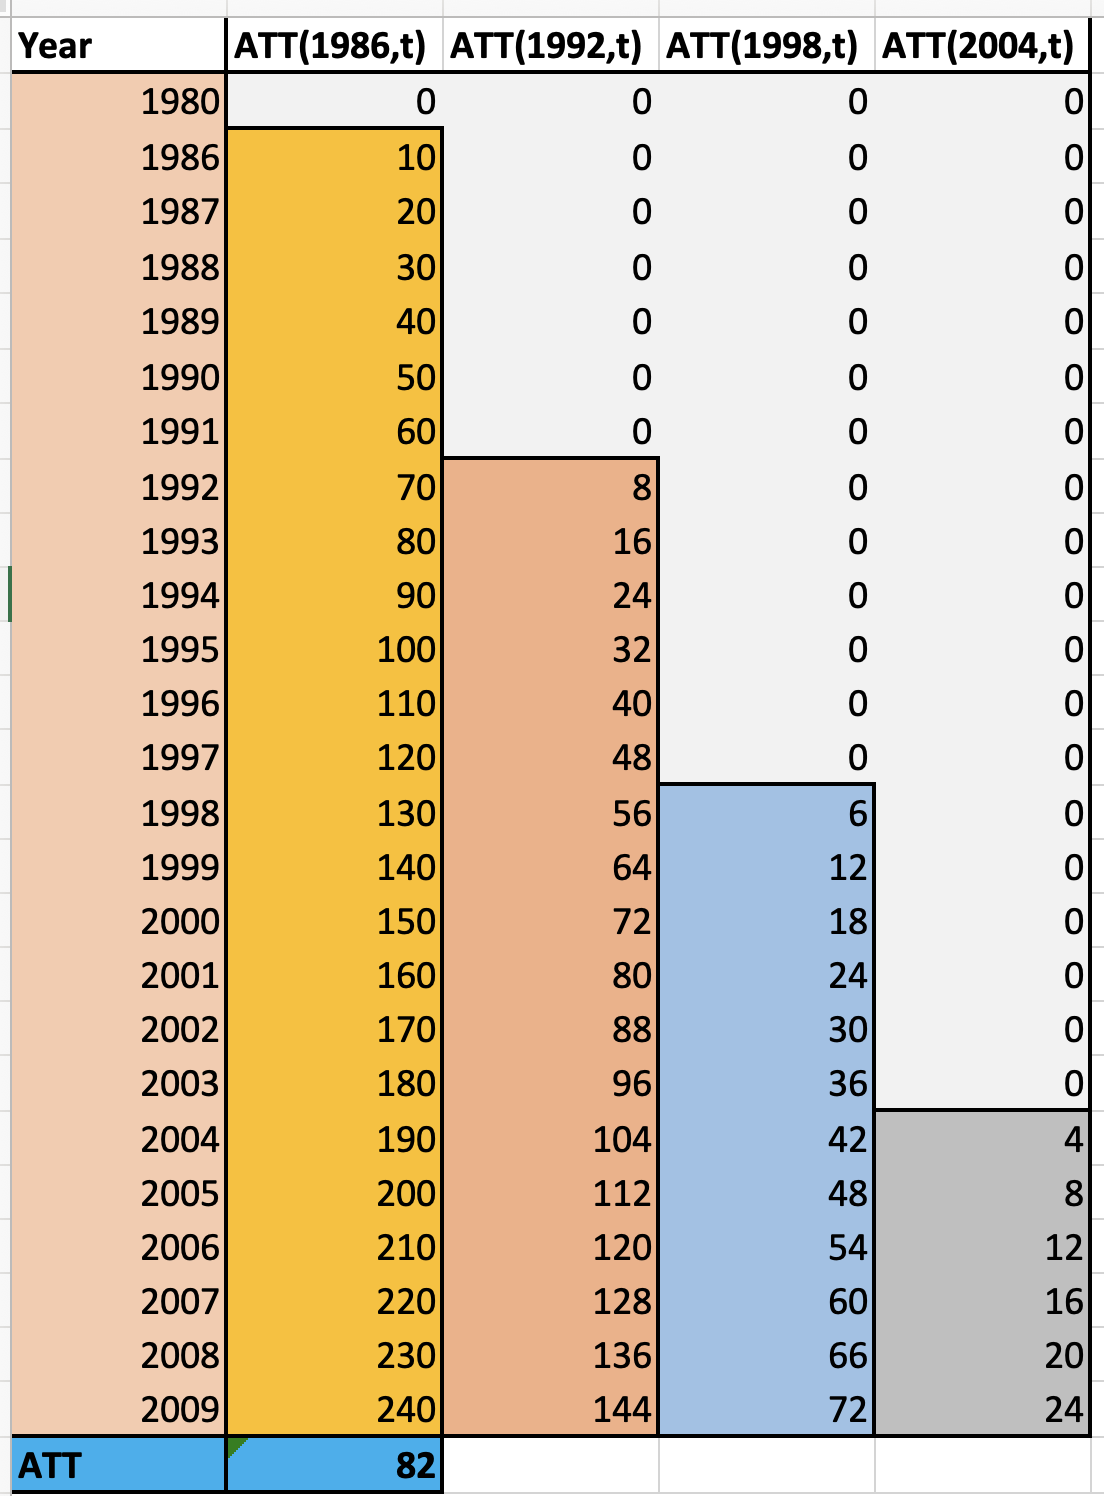
\includegraphics[height=6.5cm, width=5.5cm]{./lecture_includes/baker_attgt}
           \column{0.38\linewidth}
            Each cell contains that group's ATT(g,t)
\begin{eqnarray*}
ATT(g,t) = E[Y_t^1 - Y_t^0 | G_g=1]
\end{eqnarray*}CS identifies all feasible ATT(g,t)
         \end{columns} 
    \end{frame}




\begin{frame}{Group-time ATT}

Group-time ATT is the ATT for a specific group and time
\begin{itemize}
\item Groups are basically cohorts of units treated at the same time
\item Group-time ATT estimates are simple (weighted) differences in means
\item Does not directly restrict heterogeneity with respect to observed covariates, timing or the evolution of treatment effects over time
\item Allows us ways to choose our aggregations
\item Inference is the bootstrap
\end{itemize}

\end{frame}



\begin{frame}{Notation}

\begin{itemize}
\item $T$ periods going from $t=1, \dots, T$
\item Units are either treated ($D_t=1$) or untreated ($D_t=0$) but once treated cannot revert to untreated state
\item $G_g$ signifies a group and is binary.  Equals one if individual units are treated at time period $t$.
\item $C$ is also binary and indicates a control group unit equalling one if ``never treated'' (can be relaxed though to ``not yet treated'')
	\begin{itemize}
	\item Recall the problem with TWFE on using treatment units as controls
	\end{itemize}
\item Generalized propensity score enters into the estimator as a weight: $$\widehat{p(X)} = Pr(G_g=1 | X,G_g+C=1)$$
\end{itemize}

\end{frame}

\begin{frame}{Assumptions}

Assumption 1: Sampling is iid (panel data, but repeated cross-sections are possible) \\
\bigskip
Assumption 2: Conditional parallel trends (for either never treated or not yet treated) \\
\begin{eqnarray*}
E[Y_t^0 - Y_{t-1}^0 | X,G_g=1] = [Y_t^0 - Y_{t-1}^0 | X,C=1] 
\end{eqnarray*}
\bigskip
Assumption 3: Irreversible treatment \\
Assumption 4: Common support (propensity score) \\
\bigskip
Assumption 5: Limited treatment anticipation (i.e., treatment effects are zero pre-treatment)

\end{frame}

\begin{frame}{CS Estimator (the IPW version)}

\begin{eqnarray*}
ATT(g,t) = E \bigg [ \bigg ( \frac{G_g}{E[G_g]} - \frac{ \frac{\hat{p}(X)C}{1-\hat{p}(X)}}{E \bigg [ \frac{\hat{p}(X)C}{1-\hat{p}(X)} \bigg ]} \bigg ) (Y_t - Y_{g-1} ) \bigg ) \bigg ]
\end{eqnarray*}

This is the inverse probability weighting estimator.  Alternatively, there is an outcome regression approach and a doubly robust. Sant'Anna recommends DR.  CS uses the never-treated or the not-yet-treated as controls but never the already-treated 
\end{frame}




\begin{frame}{Aggregated vs single year/group ATT}

\begin{itemize}
\item The method they propose is really just identifying very narrow ATT per group time.
\item But we are often interested in  more aggregate parameters, like the ATT across all groups and all times
\item They present two alternative methods for building ``interesting parameters'' 
\item Inference from a bootstrap
\end{itemize}


\end{frame}



\begin{frame}{Group-time ATT }
             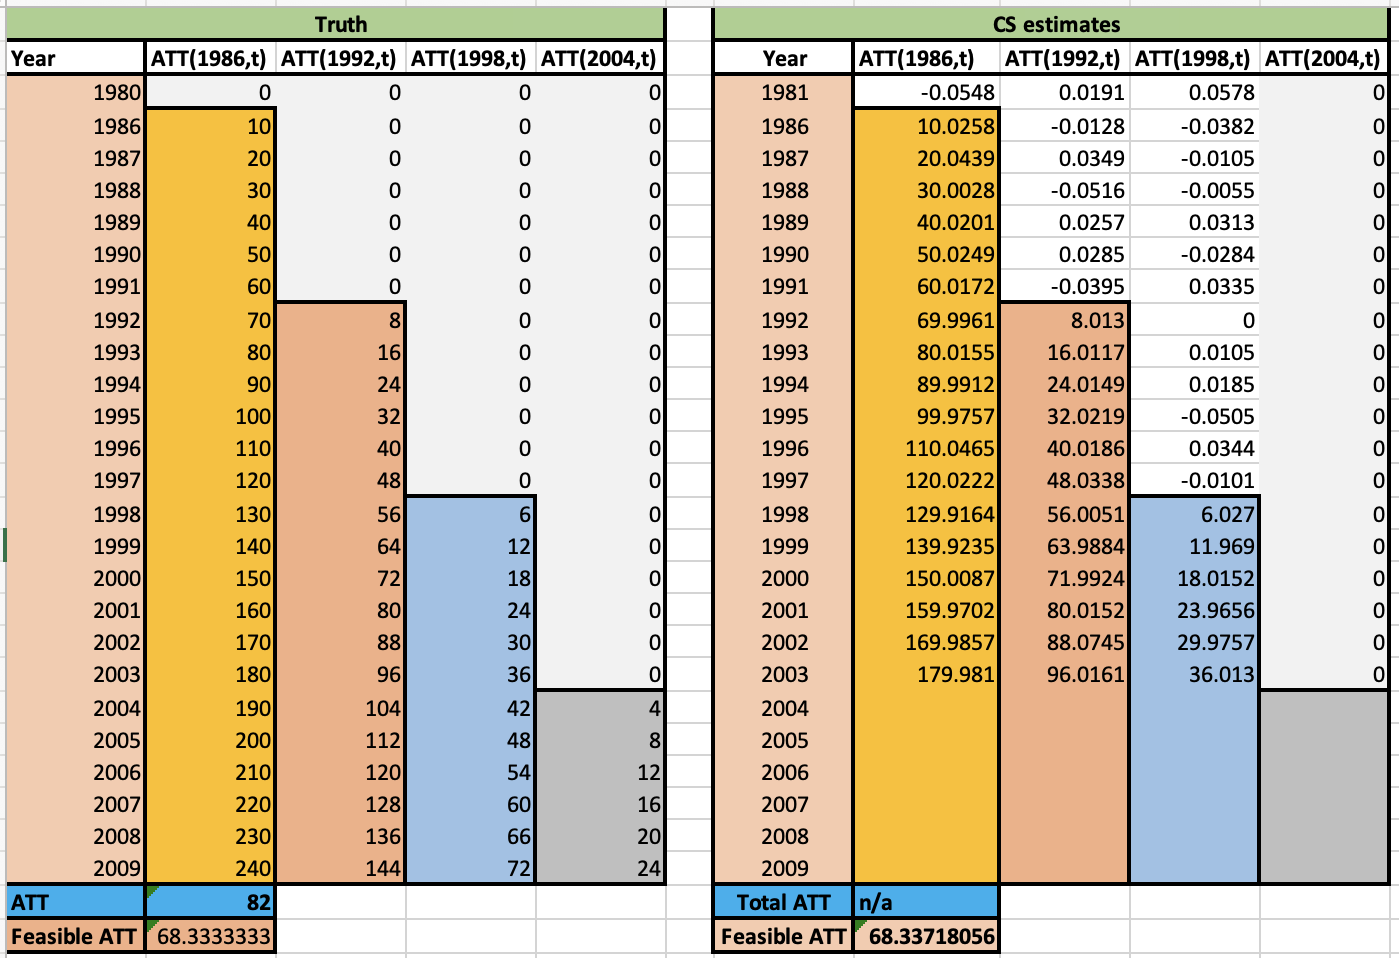
\includegraphics[scale=0.45]{./lecture_includes/baker_attgt_cs}

Question: Why didn't CS estimate all ATT(g,t)? What is ``feasible ATT''?

\end{frame}

\begin{frame}{Reporting results}
\begin{table}[htbp]\centering
\small
\caption{Estimating ATT using only pre-2004 data}
\begin{center}
\begin{tabular}{l*{5}{c}}
\hline
\multicolumn{1}{l}{\textbf{}}&
\multicolumn{1}{c}{\textbf{(Truth)}}&
\multicolumn{1}{c}{\textbf{(TWFE)}}&
\multicolumn{1}{c}{\textbf{(CS)}}&
\multicolumn{1}{c}{\textbf{(SA)}}&
\multicolumn{1}{c}{\textbf{(BJS)}}\\
\hline
$\widehat{Feasible\ ATT}$  & 68.33    & 26.81 *** & 68.34*** &&\\
\hline
\end{tabular}
\end{center}
\end{table}

TWFE is no longer negative, interestingly, once we eliminate the last group (giving us a never-treated group), but is still suffering from attenuation bias. 

\end{frame}



\subsection{SA}

\begin{frame}{Event study and differential timing}

\begin{itemize}
\item Sometimes we care about a simple summary, and sometimes we care about separating it out in time and sometimes in even more interesting ways
\item Event studies with one treatment group and one untreated group were relatively straightforward
\item Interact treatment group with calendar date to get a series of leads and lags
\item But when there are more than one treatment group, specification challenges emerge
\end{itemize}

\end{frame}




\begin{frame}{Replicated from a project of mine}

	\begin{figure}
	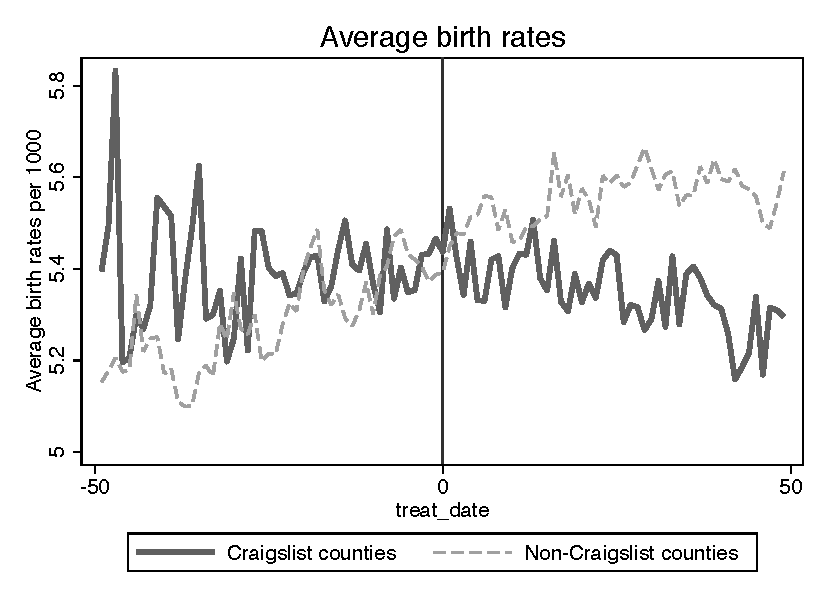
\includegraphics[scale=0.5]{./lecture_includes/dd.pdf}
	\caption{Roll out of Craigslist ``personal ads'' for casual intimate encounters and birth rates using the ``randomized treatment assignment'' approach (Anderson, et al. 2013) for visualization}
	\end{figure}

\end{frame}

\begin{frame}{Event study specification with TWFE}


\begin{eqnarray*}
Y_{i,t} = \alpha_i + \delta_t + \sum_{g \in G} \mu_g1\{t-E_i \in g \} + \varepsilon_{i,t}
\end{eqnarray*}

\bigskip

Coefficient $\mu_g$ on a dummy measuring the number of years prior to or after that unit was treated.  

\end{frame}

\begin{frame}[plain]
	\begin{figure}
	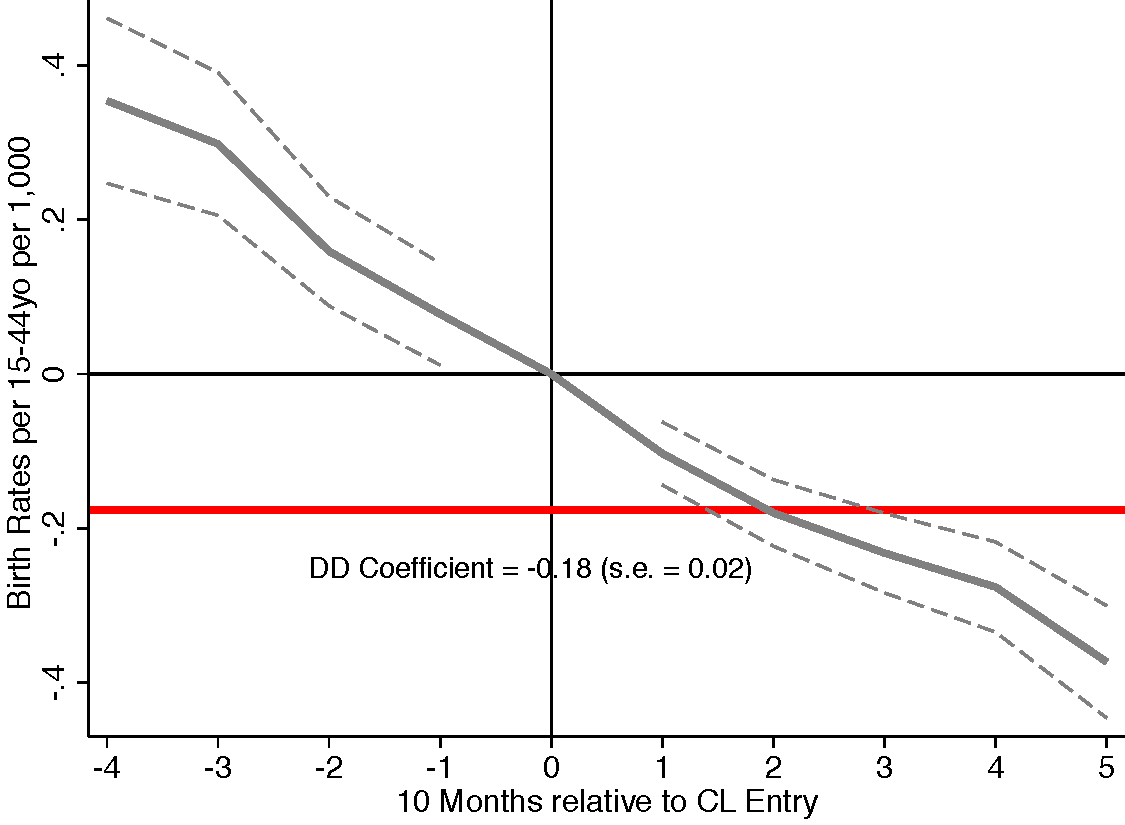
\includegraphics[scale=0.5]{./lecture_includes/br1544.pdf}
	\end{figure}
	
Same data as a couple slides ago, leads don't look good, so I abandoned the project. 
	
\end{frame}

\begin{frame}{Bias of TWFE Event Study Specification}

\begin{itemize}
\item Bacon only focused on the static specification, and that's where the biases due to dynamics revealed itself
\item He was unable to get into the leads and lags using the FWL method he was using (``it's hard!'' - Bacon)
\item Sophie Sun and Sarah Abraham did though -- prompted by a stray comment by their professor
\item But they also unlike Bacon present a solution (which is like CS, but discovered independently)
\end{itemize}

\end{frame}



\begin{frame}{Sun and Abraham 2020}

	\begin{enumerate}
	\item SA shows a decomposition of the population regression coefficient on event study leads and lags with differential timing estimated with TWFE
	\item They show that the population regression coefficient is ``contaminated'' by information from other leads and lags (which is then later generalized by Goldsmith-Pinkham, Hull and Kolsar 2022)
	\item SA presents an alternative estimator that is a version of CS only using the ``last cohort'' as the treatment group (not the not-yet-treated)
	\item Derives the variance of the estimator instead of bootstrapping, handles covariates differently than CS, but otherwise identical
	\end{enumerate}

\end{frame}

\begin{frame}{Summarizing (cont.)}

\begin{itemize}
\item Under homogenous treatment profiles, weights sum to zero and``cancel out'' the treatment effects from other periods 
\item Under treatment effect heterogeneity, they do not cancel out and leads and lags are biased
\item They present a 3-step TWFE based alternative estimator which addresses the problems that they find
\end{itemize}

\end{frame}


\begin{frame}{Some notation and terms}

\begin{itemize}
\item As people often \textbf{bin} the data, we allow a lead or lag $l$ to appear in bin $g$ so sometimes they use $g$ instead of $l$ or $l \in g$
\item Building block is the ``cohort-specific ATT'' or $CATT_{e,l}$ -- same as ATT(g,t)
\item Our goal is to estimate $CATT_{e,l}$ with population regression coefficient $\mu_l$
\item They focus on irreversible treatment where treatment status is non-decreasing sequence of zeroes and ones
\end{itemize}

\end{frame}



\begin{frame}{Difficult notation (cont.)}

\begin{itemize}
\item The $\infty$ symbol is used to either describe the group ($E_i=\infty$) or the potential outcome ($Y^{\infty}$)
\item $Y^{\infty}_{i,t}$ is is the potential outcome for unit $i$ if it had never received treatment (versus received it later), also called the baseline outcome
\item Other counterfactuals are possible -- maybe unit $i$ isn't ``never treated'' but treated later in counterfactual
\end{itemize}
\end{frame}

\begin{frame}{More difficult notation (cont.)}

\begin{itemize}
\item Treatment effects are the difference between the observed outcome relative to the never-treated counterfactual outcome: $Y_{i,t} - Y^{\infty}_{i,t}$
\item We can take the average of treatment effects at a given relative time period across units first treated at time $E_i=e$ (same cohort) which is what we mean by $CATT_{e,l}$
\item Doesn't use $t$ index time (``calendar time''), rather uses $l$ which is time until or time after treatment date $e$ (``relative time'')
\item Think of it as ${l}=$year - treatment date
\end{itemize}

\end{frame}



\begin{frame}{Definition 1}

\textbf{Definition 1:} The cohort-specific ATT $l$ periods from initial treatment date $e$ is:

\begin{eqnarray*}
CATT_{e,l} = E[Y_{i,e+l} - Y^{\infty}_{i,e+l} | E_i=e]
\end{eqnarray*}

\bigskip

Fill out the second part of the Group-time ATT exercise together.

\end{frame}

\begin{frame}{TWFE assumptions}

\begin{itemize}
\item For consistent estimates of the coefficient leads and lags using TWFE model, we need three assumptions
\item For SA and CS, we only need two
\item Let's look then at the three
\end{itemize}

\end{frame}


\begin{frame}{Assumption 1: Parallel trends}

\textbf{Assumption 1: Parallel trends in baseline outcomes}: $E[Y^{\infty}_{i,t} - Y^{\infty}_{i,s} | E_i = e ]$ is the same for all $e \in supp(E_i)$ and for all $s$, $t$ and is equal to $E[Y^{\infty}_{i,t} - Y^{\infty}_{i,s} ]$

\bigskip

Lead and lag coefficients are DiD equations but once we invoke parallel trends they can become causal parameters.  This reminds us again how crucial it is to have  appropriate controls

\end{frame}


\begin{frame}{Assumption 2: No anticipation}

\textbf{Assumption 2: No anticipator behavior in pre-treatment periods}: There is a set of pre-treatment periods such that $E[Y_{i,e+l}^e - Y_{i,e+l}^{\infty} | E_i = e]=0$ for all possible leads.

\bigskip

Essentially means that pre-treatment, the causal effect is zero.  Most plausible if no one sees the treatment coming, but even if they see it coming, they may not be able to make adjustments that affect outcomes

\end{frame}


\begin{frame}{Assumption 3: Homogeneous dynamics}

\textbf{Assumption 3: Treatment effect profile homogeneity}: For each relative time period $l$, the $CATT_{e,l}$ doesn't depend on the cohort and is equal to $CATT_l$. 


\end{frame}

\begin{frame}{Homogeneous dynamics}

\begin{itemize}
\item Assumption 3 allows for dynamic treatment effects; it just requires that different cohorts have the \emph{same} dynamics
\item Cohorts may differ in their covariates which affect how they respond to treatment (e.g., if treatment effects vary with age, and there is variation in age across units first treated at different times, then there will be heterogeneous treatment effects)
\item Original SA does not include covariates, though code has often been developed to include it -- just remember what we saw with the double robust discussion
\item Treatment effect doesn't rule out parallel trends -- parallel trends turns simple DiD into causal parameters
\end{itemize}

\end{frame}

\begin{frame}{Event study model}

Dynamic TWFE model

\begin{eqnarray*}
Y_{i,t} = \alpha_i + \delta_t + \sum_{g \in G} \mu_g1\{t-E_i \in g \} + \varepsilon_{i,t}
\end{eqnarray*}

\bigskip

We are interested in the properties of $\mu_g$ under differential timing as well as whether there are any never-treated units

\end{frame}



\begin{frame}[plain, shrink=20]
\begin{center}
\textbf{Interpreting $\widehat{\mu_g}$ under no to all assumptions}
\end{center}

\textbf{Proposition 1 (no assumptions):} The population regression coefficient on relative period bin $g$ is a linear combination of differences in trends from its own relative period $l \in g$, from relative periods $l \in g'$ of other bins $g' \neq g$, and from relative periods excluded from the specification (e.g., trimming). 

\begin{eqnarray*}
\mu_g &=& \underbrace{\sum_{l \in g} \sum_{e} w^g_{e,l} \big ( E[Y_{i,e+l} - Y^{\infty}_{i,0} | E_i = e] - E[Y^{\infty}_{i,e+l} - Y^{\infty}_{i,0}] \big )}_{\mathclap{\text{Targets}}} \\
&+& \underbrace{\sum_{g' \neq g} \sum_{l \in g'} \sum_e w^g_{e,l} \big ( E[Y_{i,e+l} - Y^{\infty}_{i,0} | E_i=e] - E[Y^{\infty}_{i,e+l} - Y^{\infty}_{i,0}] \big )}_{\mathclap{\text{Contamination from other leads and lags}}} \\
&+&  \underbrace{\sum_{l \in g^{excl}} \sum_{e} w^g_{e,l} \big ( E[Y_{i,e+l} - Y^{\infty}_{i,0} | E_i=e] - E[Y^{\infty}_{i,e+l} - Y^{\infty}_{i,0}] \big )}_{\mathclap{\text{Contamination from dropped periods}}} 
\end{eqnarray*}

\bigskip


\end{frame}

\begin{frame}{Weight ($w^g_{e,l}$) summation cheat sheet}

\begin{enumerate}
\item For relative periods of $\mu_g$ own $l \in g$, $\sum_{l \in g}\sum_ew^g_{e,l}=1$
\item For relative periods belonging to some other bin $l\in g'$ and $g' \neq g$, t $\sum_{l \in g'}\sum_ew^g_{e,l} = 0$
\item For relative periods not included in $G$, $\sum_{l \in g^{excl}} \sum_e w^g_{e,l} = -1$
\end{enumerate}

\end{frame}




\begin{frame}{Estimating the weights}

Regress $D^l_{i,t} \times 1\{E_i=e \}$ on:

\begin{enumerate}
\item all bin indicators included in the main TWFE regression, 
\item $\{ 1\{ t-E_i \in g \} \}_{g \in G}$(i.e., leads and lags) and 
\item the unit and time fixed effects
\end{enumerate}

\end{frame}


\begin{frame}{Still biased under parallel trends}

\textbf{Proposition 2}: Under the parallel trends only, the population regression coefficient on the indicator for relative period bing $g$ is a linear combination of $CATT_{e,l \in g}$ as well as $CATT_{d,l'}$ from other relative periods $l' \notin g$ with the same weights stated in Proposition 1:

\begin{eqnarray*}
\mu_g &=& \underbrace{\sum_{l \in g} \sum_e w^g_{e,l} CATT_{e,l}}_{\mathclap{\text{Desirable}}} \\
&& + \underbrace{\sum_{g' \neq g, g' \in G} \sum_{l' \in g'} \sum_e w^g_{e,l'}  CATT_{e,l'}}_{\mathclap{\text{Bias from other specified bins}}} \\
&&+ \underbrace{\sum_{l' \in g^{excl}} \sum_e w^g_{e,l'} CATT_{e,l'}}_{\mathclap{\text{Bias from dropped relative time indicators}}}
\end{eqnarray*}



\end{frame}


\begin{frame}{Still biased under parallel trends and no anticipation}

\textbf{Proposition 3}: If parallel trends holds and no anticipation holds for all $l<0$ (i.e., no anticipatory behavior pre-treatment), then the population regression coefficient $\mu_g$ for $g$ is a linear combination of post-treatment $CATT_{e,l'}$ for all $l' \geq 0$.

\begin{eqnarray*}
\mu_g &=& \sum_{l' \in g, l' \geq 0} \sum_e w^g_{e,l'} CATT_{e,l'} \\
&&+ \sum_{g' \neq g,g' \in G} \sum_{l' \in g', l' \geq 0} \sum_e w^g_{e,l'} CATT_{e,l'} \\
&&+ \sum_{l' \in g^{excl},l' \geq 0} \sum_e w^g_{w,l'} CATT_{e,l'}
\end{eqnarray*}

\end{frame}

\begin{frame}{Proposition 3 comment}

Notice how once we impose zero pre-treatment treatment effects, those terms are gone (i.e., no $l \in g, l<0$).  But the second term remains unless we impose treatment effect homogeneity (homogeneity causes terms due to weights summing to zero to cancel out). Thus $\mu_g$ may be non-zero for pre-treatment periods \emph{even though parallel trends hold in the pre period.}

\end{frame}

\begin{frame}{Proposition 4}

\textbf{Proposition 4}: If parallel trends and treatment effect homogeneity, then $CATT_{e,l}=ATT_l$ is constant across $e$ for a given $l$, and the population regression coefficient $\mu_g$ is equal to a linear combination of $ATT_{l \in g}$, as well as $ATT_{l' \notin g}$ from other relative periods

\begin{eqnarray*}
\mu_g &=& \sum_{l \in g} w^g_l ATT_l \\
&&+ \sum_{g' \neq g} \sum_{l' \in g'} w^g_{l'} ATT_{l'} \\
&&+ \sum_{l' \in g^{excl}} w^g_{l'}ATT_{l'}
\end{eqnarray*}


\end{frame}

\begin{frame}{Simple example}


Balanced panel $T=2$ with cohorts $E_i \in \{1,2 \}$. For illustrative purposes, we will include bins $\{-2,0\}$ in our calculations but drop $\{-1,1\}$. 


\end{frame}

\begin{frame}{Simple example}

\begin{eqnarray*}
\mu_{-2} &=& \underbrace{CATT_{2,-2}}_{\mathclap{\text{own period}}} + \underbrace{\frac{1}{2}CATT_{1,0} - \frac{1}{2} CATT_{2,0}}_{\mathclap{\text{other included bins}}} \\
&&+ \underbrace{ \frac{1}{2} CATT_{1,1} - CATT_{1,-1} - \frac{1}{2} CATT_{2,-1} }_{\mathclap{\text{Excluded bins}}}
\end{eqnarray*}

\begin{itemize}
\item Parallel trends gets us to all of the $CATT$
\item No anticipation makes $CATT=0$ for all $l<0$ (all $l<0$ cancel out)
\item Homogeneity cancels second and third terms
\item Still leaves $\frac{1}{2} CATT_{1,1}$ -- you chose  to exclude a group with a treatment effect
\end{itemize}Lesson: drop the relative time indicators on the left, not things on the right, bc lagged effects will contaminate through the excluded bins


\end{frame}


\begin{frame}{Interacted weighted estimator}


\begin{itemize}
\item Sun and Abraham (2020) propose a 3-step interacted weighted estimator (IW) using last treated group as control group
\item Contrast with Callaway and Sant'Anna (2020) estimate group-time ATT which can be a weighted average over relative time periods too but uses ``not-yet-treated'' as control
\item They are numerical identical with balanced panels, no covariates and using the never treated as controls
\end{itemize}

\end{frame}




\begin{frame}{Interaction weighted estimator}

\begin{itemize}
\item \textbf{Step one}: Do this DD regression and hold on to $\widehat{\delta}_{e,l}$
\end{itemize}

\begin{eqnarray*}
Y_{i,t} = \alpha_i + \lambda_t + \sum_{e \notin C} \sum_{l \neq -1} \delta_{e,l} \big (1 \{ E_i = e \} \cdot D_{i,t}^l \big ) + \varepsilon_{i,t}
\end{eqnarray*}


\bigskip

Can use never-treated or last-treated cohort; just can't accommodate the not-yet-treated. Drop always treated. The $\delta_{e,l}$ is a DD estimator for $CATT_{e,l}$ with particular choices for pre-period and cohort controls

\end{frame}


\begin{frame}{Interaction weighted estimator}

\begin{itemize}
\item \textbf{Step two}: Estimate weights using sample shares of each cohort in the relevant periods:
\end{itemize}

\begin{eqnarray*}
Pr(E_i=e|E_i \in [-l,T-l])
\end{eqnarray*}

\end{frame}

\begin{frame}{Interaction weighted estimator}

\begin{itemize}
\item \textbf{Step three}: Take a weighted average of estimates for $CATT_{e,l}$ from Step 1 with weight estimates from step 2
\end{itemize}


\begin{eqnarray*}
\widehat{v}_g = \frac{1}{|g|} \sum_{l \in g} \sum_e \widehat{\delta}_{e,l} \widehat{Pr} \{ E_i=e | E_i \in [-l,T-l]\}
\end{eqnarray*}


\end{frame}

\begin{frame}{Consistency and Inference}


\begin{itemize}
\item Under parallel trends and no anticipation, $\widehat{\delta}_{e,l}$ is consistent, and sample shares are also consistent estimators for population shares. 
\item Thus IW estimator is consistent for a weighted average of $CATT_{e,l}$ with weights equal to the share of each cohort in the relevant period(s).
\item They show that each IW estimator is asymptotically normal and derive its asymptotic variance. Doesn't rely on bootstrap like CS.
\end{itemize}

\end{frame}

\begin{frame}{DD Estimator of CATT}

\textbf{Definition 2}: DD estimator with pre-period $s$ and control cohorts $C$ estimates $CATT_{e,l}$ as:

\begin{eqnarray*}
\widehat{\delta_{e,l}} = \frac{ E_N \big [ \big ( Y_{i, e+l} - Y_{i,s} \big ) \times 1\{E_i=e\} \big ]}{E_N[1 \{E_i=e\} ]} - \frac{E_N \big [ \big ( Y_{i,e+l} - Y_{i,s} \big ) \times 1 \{E_i \in C \} ]}{E_N [1 \{ E_i \in C \}]}
\end{eqnarray*}


\textbf{Proposition 5}: If parallel trends and no anticipation both hold for all pre-periods, then the DD estimator using any pre-period and non-empty control cohorts (never-treated or not-yet-treated) is an unbiased estimate for $CATT_{e,l}$

\end{frame}

\begin{frame}{Software}

\begin{itemize}
\item \textbf{Stata}: eventstudyinteract (can be installed from ssc)
\item \textbf{R}: fixest with subab() option (see \url{https://lrberge.github.io/fixest/reference/sunab.html/})
\end{itemize}


\end{frame}


\begin{frame}{Reporting results}
\begin{table}[htbp]\centering
\small
\caption{Estimating ATT}
\begin{center}
\begin{tabular}{l*{5}{c}}
\hline
\multicolumn{1}{l}{\textbf{}}&
\multicolumn{1}{c}{\textbf{(Truth)}}&
\multicolumn{1}{c}{\textbf{(TWFE)}}&
\multicolumn{1}{c}{\textbf{(CS)}}&
\multicolumn{1}{c}{\textbf{(SA)}}&
\multicolumn{1}{c}{\textbf{(BJS)}}\\
\hline
$\widehat{Feasible\ ATT}$  & 68.33    & 26.81*** & 68.34*** & 68.33***&\\
\hline
\end{tabular}
\end{center}
\end{table}

\end{frame}

\begin{frame}{Computing relative event time leads and lags }
             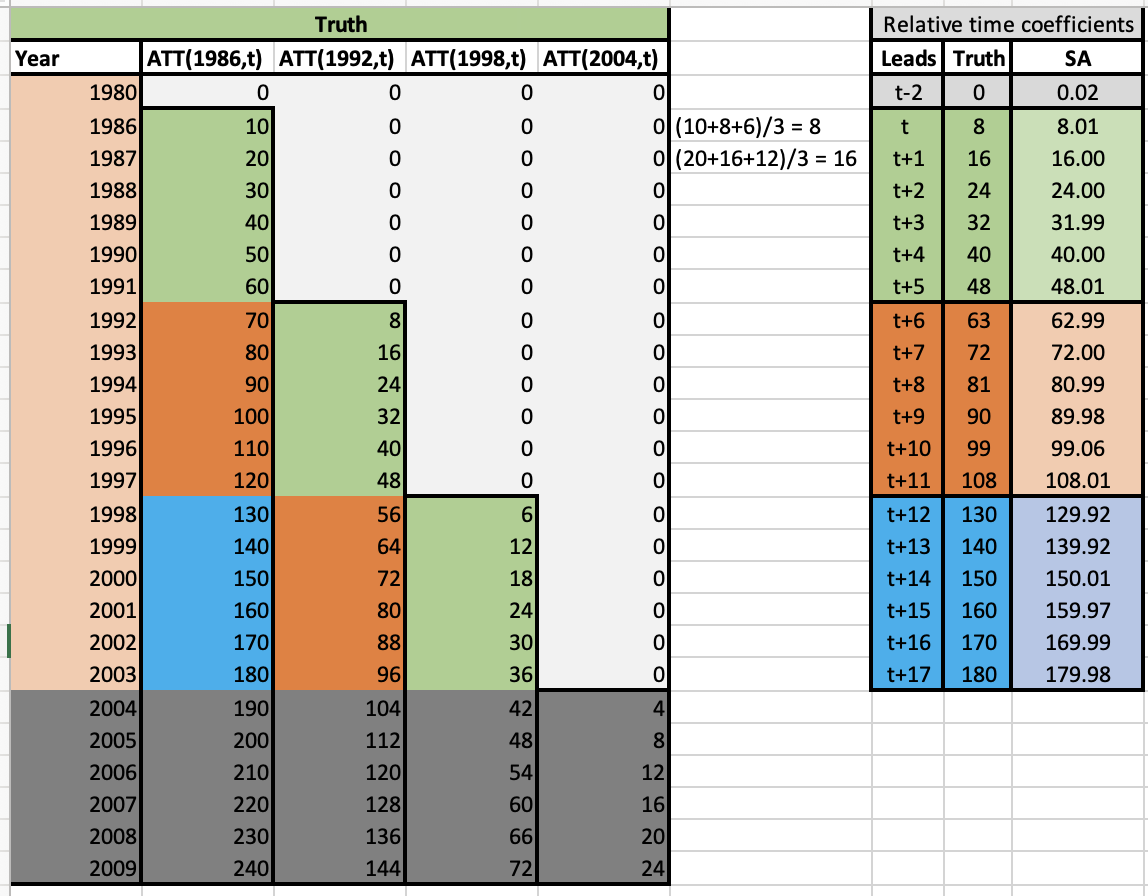
\includegraphics[scale=0.45]{./lecture_includes/sa_leads}

Two things to notice: (1) there only 17 lags with robust models but will be 24 with TWFE; (2) changing colors mean what?

\end{frame}

\begin{frame}{Comparing TWFE and SA }

\begin{figure}
\begin{center}
             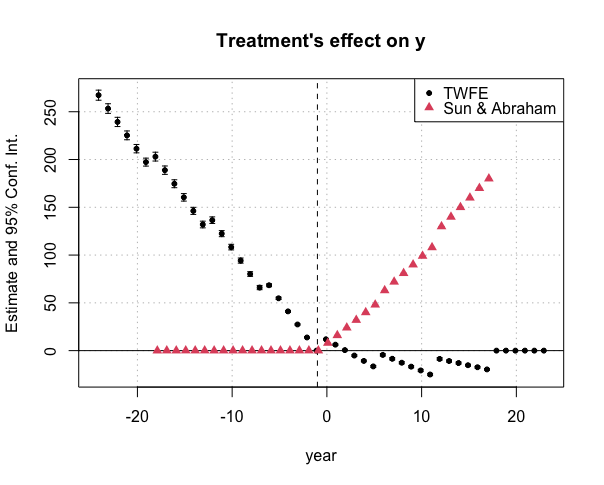
\includegraphics[scale=0.4]{./lecture_includes/twfe_sa_event}
\end{center}
\end{figure}

Question: why is TWFE \emph{falling} pre-treatment?  Why is SA rising, but jagged, post-treatment?

\end{frame}

\subsection{dCH}

\begin{frame}{de Chaisemartin and D'Haultfoeulle 2020}

de Chaisemartin and D'Haultfouelle 2020 (dCdH) is different from the other papers in several ways
	\begin{itemize}
	\item Like SA, it's a diagnosis and a cure
	\item TWFE decomposition shows coefficient a weighted average of underlying treatment effects, but weights can be negative negating causal interpretation
	\item Propose a solution for both static and dynamic specification which does not use already treated as controls
	\item Treatment can turn on and off
	\end{itemize}

\end{frame}


\begin{frame}{Comment on Bacon}

\begin{itemize}
\item Recall the Bacon decomposition -- TWFE coefficients are decomposed into weighted average of all underlying 2x2s. Weights were non-negative and summed to one.
\item But this decomposition was more a numerical decomposition -- what exactly adds up to equal the TWFE coefficient using the data we observe?
\item Bacon's decomposition is not ``theoretical'' -- not in the way that other decompositions are. He is just explaining what OLS ``does'' when it calculates $\widehat{\delta}$
\item Just explains what comparisons OLS is using to calculate the TWFE coefficient -- just peels back the curtain.
\end{itemize}

\end{frame}

\begin{frame}{Negative weights}

\begin{itemize}
\item dCdH impose causal assumptions and try a different decomposition strategy
\item Uses as its building block the unit-specific treatment effects
\item Their decomposition will reveal negative weights on the underlying treatment effects (similar to negative weight on dynamics with Bacon)
\item Remember though: the Bacon decomposition weights were \emph{always} positive, because they were numerical weights (not theoretical weights) on the underlying 2x2s (not the treatment effects)
\end{itemize}

\end{frame}

\begin{frame}{Turning on and off}

\begin{itemize}
\item CS and SA both require interventions to turn on and stay on
\item dCdH allows for ``switching'' on and off 
\item Before we move quickly into that, please note that the researcher bears the burden of knowing whether in fact you want to impose symmetry on turning on and off
\item Roe v Wade ``turned on'' legalized abortion and 2022 it was ``turned off'' -- do we want to treat these as simply a single policy flipping of the switch or two separate policies?
\end{itemize}

\end{frame}

\begin{frame}{dCdH notation}

\begin{itemize}
\item Individual treatment effects (iow, not the group-time ATT): $$\Delta^g_{i,t} = Y^1_{i,t} - Y^\infty_{i,t}$$ but where the treatment is in time period $g$. Notice --it's not the ATT (it's $i$ individual treatment effect)
\item with defined error term as $\varepsilon_{i,t}$: $$D_{i,t} = \alpha_i + \alpha_t + \varepsilon_{i,t}$$
\item Weights: $$w_{i,t} = \frac{\varepsilon_{i,t}}{\frac{1}{N^T} \sum_{i,t:D_{i,t}=1} \varepsilon_{i,t}}$$
\end{itemize}

\end{frame}

\begin{frame}{Parallel trend assumption}

\begin{block}{Strong unconditional PT}
Assume that for every time period $t$ and every group $g,g'$, $$E[Y^\infty_t - Y^\infty_{t-1}|G=g] = E[Y^\infty_t - Y^\infty_{t-1}|G=g'] $$
\end{block}Assume parallel trends for every unit in every cohort in every time period.

\bigskip

What then does TWFE estimate with differential timing?

\end{frame}

\begin{frame}{dCdH Theorem}

\begin{block}{Theorem -- dCdH decomposition}
Assuming SUTVA, no anticipation and the strong PT, then let $\delta$ be the TWFE estimand associated with $$Y_{i,t} = \alpha_i + \alpha_t + \delta D_{i,t} + \varepsilon_{i,t}$$Then it follows that $$\delta = E \bigg [ \sum_{i,t:D_{i,t}=1} \frac{1}{N^T} w_{i,t} \cdot \Delta_{i,t}^g \bigg ] $$ where $\sum_{i,t:D_{i,t}=1} \frac{w_{i,t}}{N^T} = 1$ but $w_{i,t}$ can be negative
\end{block}

\end{frame}

\begin{frame}{Origins}

\begin{itemize}
\item So once you run that specification, $\widehat{\delta}$ is going to recover a ``non-convex average'' over all unit level treatment effects (weights can be negative, more on this). 
\item Not sure who came first, because there were working papers before publications, but my understanding is dCdH was the first to prove this
\item Very important theorem -- established the ``no sign flip property'' for OLS with differential timing in the canonical static specification
\end{itemize}

\end{frame}


\begin{frame}{Negative weights}

\begin{itemize}
\item Very common now to hear about negative weights, and furthermore, that negative weights wipe out any causal interpretation, but why?
\item Thought experiment: imagine every unit gained from the treatment, but their treatment effect when estimated was multiplied by a negative number
\item It's possible it could flip the sign, but it would definitely at least pull the estimate away from the true effect
\item This is dangerous -- and it's caused by the forbidden contrasts (comparing treated to already treated) which is what the canonical TWFE static specification is doing (for many of us unknowingly)
\end{itemize}

\end{frame}



\begin{frame}{Negative weights}

\begin{itemize}
\item Doesn't always pose a problem, but no proofs for this intuition known yet
\item A large number of never-treated seems to make this less an issue
\item Shrinking the spacing between treatment dates also can drive it down
\item But does that mean that TWFE works, and what does it mean to work?
\item TWFE still even when all the weights are positive the weighted average may not aggregate to what we think it does
\end{itemize}

\end{frame}

\begin{frame}{Weighting}

\begin{itemize}
\item The weights in OLS all come out of the model itself, \emph{not the economic question}
\item The economic question is ``what parameter do you want? What does it look like? Who is in it?''
\item And when you define the parameter up front, you've more or less defined the economic question you're asking
\item But OLS sort of ignores your question and just gives you what it wants
\end{itemize}

\end{frame}

\begin{frame}{Weighting}

\begin{itemize}
\item What makes something a good vs a bad weight?
\item Not being negative is the absolute minimal requirement
\item But it's also not a good sign if you can't really explain the weights
\end{itemize}

\end{frame}

\begin{frame}{dCdH Solution}

\begin{itemize}
\item dCdH propose an alternative that doesn't have the problems of TWFE -- both avoiding negative weights and improving interpretability
\item Recall, their model can handle reversible treatments

\end{itemize}

\end{frame}


\subsection{Imputation based robust estimator}



\begin{frame}{Imputation method by BJS (2023)}

\begin{itemize}

\item The origin of the robust diff-in-diff papers identifying pathologies in TWFE was Borusyak and Jaravel (2016) working paper
\item Both problems with static and dynamic specifications were discussed, and the identification of the ``already treated'' as controls
\item Paper remained in working paper until 2021 when Jan Speiss was brought on; the team developed a new estimator (now published at Restud)
\item We will focus primarily on the estimator, to avoid redundancies

\end{itemize}

\end{frame}



\begin{frame}{ATT parameter}

Estimation target will be unit level treatment effects (as opposed to group-time ATT) aggregated to a higher level like the ATT:

\begin{eqnarray*}
\tau_w = \sum_{it \in \Omega_{1}}w_{it}\tau_{it} = w'_1\tau
\end{eqnarray*}

\bigskip

Note the weights -- they need not add up to one.  Weights could be $\frac{1}{N}$ for all $it \in \Omega_1$. We have a number of options. 


\end{frame}

\begin{frame}{Standard TWFE Assumptions}

\begin{enumerate}
\item Parallel trends -- expressed as a TWFE model with unit-level parallel trends (stronger than needed)
\item No anticipation
\item Homogenous treatment effects
\item SUTVA (as always)
\end{enumerate}

\end{frame}

\begin{frame}{A1: Parallel trends}

\textbf{Assumption 1: Parallel trends}. There exist non-stochastic $\alpha_i$ and $\beta_t$ such that:

$$Y_{it}(0) = \alpha_i + \beta_t + \varepsilon_{it}$$with $$E[\varepsilon_{it}]=0$$for all $it \in \Omega$. Can be extended (e.g., unit-specific trends). Only imposes restrictions on $Y(0)$, not treatment effects themselves. Notice how it is a TWFE assumption -- it's actually the same data generating process as in baker.do.

\end{frame}

\begin{frame}{A2: No anticipation}

\begin{itemize}
\item No anticipation rules out anticipatory behavior that would cause treatment effects to materialize even before the treatment occurred:$$Y_{it} = Y_{it}(0)$$ for all $it \in \Omega_0$. 
\item Notice how as an assumption, it literally imposes $\tau=0$ for all pre-treatment periods. 
\item It's crucial for the pre-trends to be zero, far more than parallel trends, as parallel trends is \emph{only} about post-treatment from baseline, whereas event studies are about pre-trends and that's where no anticipation reigns

\end{itemize}

\end{frame}



\begin{frame}{A3: Restricted causal effects}

This is the one that places restrictions on what treatment effects can and cannot be (i.e., homogenous treatment effects). Notice the very detailed expression:

\bigskip

\textbf{Assumption 3 (Restricted causal effects)}: $B\tau0$ for a known $M \times N_1$ matrix $B$ of full row rank. 

\bigskip

If we can assume something like homogenous treatment effects, then TWFE actually is best because its ability to \emph{correctly} extrapolate will increase efficiency. But it's when A3 is not tenable or not really ex ante justified by theory that we should be worried. There's an A3' that is a slight modification. 

\end{frame}


\begin{frame}{Critique of Common Practice}

\begin{enumerate}
\item Under-identification in event studies
\item Negative weighting
\item Spurious identification of long-run casual effects
\end{enumerate}

\end{frame}

\begin{frame}{Critique: Underidentification problem}


\textbf{Lemma 1}: If there are no never-treated units, the path of [pre-treatment lead population regression coefficients] is not point identified in the fully dynamic OLS specification.  In particular. adding a linear trend to this path $\{\tau_h + k(h+1) \}$ for any $k \in R$ fits the data equally well with the fixed effects coefficients appropriately modified.

\bigskip

In english, it means you're going to have a multicollinearity problem even worse than you thought when estimating the fully dynamic event study model (i.e., dropping only one lead for all base comparisons)

\end{frame}


\begin{frame}{Underidentification of lead coefficients}

\begin{block}{Under-identification problem}
Formally the problem arises because a linear time trend $t$ and a linear term in the cohort $E_i$ (subsumed by the unit FEs) can perfectly reproduce a linear term in relative time $K_{it}=t-E_i$.  Therefore a complete set of treatment leads and lags, which is equivalent to the FE of relative time, is collinear with the unit and period FEs.
\end{block}

\bigskip

Just one additional normalization is needed -- drop $\tau_{-a}=0$ and $\tau_{-1}=0$.  This will break the multicollinearity.  We saw this in SA also.  So multiple people saw this at the same time.

\end{frame}

\begin{frame}{Under-identification and theoretical justifications}

\begin{itemize}
\item Imposing any $-a$ lead and $-1$ lead to equal zero is somewhat ad hoc.  Why those two and not some other two?
\item Recall with SA -- it mattered which ones you dropped because otherwise leads were contaminated
\item This is again about NA -- if you chose $-a$ and $-1$, then you had some theoretical reason to assume NA held for them and not some other periods
\end{itemize}

\end{frame}



\begin{frame}{Negative weighting and violations of A3}

Assume some simple static model with a single dummy for treatment.  Then they lay out a second lemma

\bigskip 
\textbf{Lemma 2}: If A1 and A2 hold, then the estimand of the static OLS specification satisfies $\tau^{static}=\sum_{it \in \Omega_1} w_{it}^{OLS}\tau_{it}$ for some weights $w_{it}^{OLS}$ that do not depend on the outcome realizations and add up to one $\sum_{it \in \Omega_1}=1$.

\bigskip

The static OLS estimand cannot be interpreted as a ``proper'' weighted average, as some weights can be negative. 

\end{frame}


\begin{frame}{Simple illustration}


\begin{table}[htb]\centering
\scriptsize
\caption{TWFE dynamics}
\centering
\begin{threeparttable}
\begin{tabular}{l*{2}{c}}
\toprule
\multicolumn{1}{l}{$E(y_{it})$ }&
\multicolumn{1}{c}{\textbf{$i=A$ }}&
\multicolumn{1}{c}{\textbf{$i=B$ }}\\
\midrule
t=1 & $\alpha_A$ & $\alpha_B$ \\
t=2 & $\alpha_A + \beta_2 + \delta_{A2}$ & $\alpha_B$ + $\beta_2$ \\
t=3 & $\alpha_A + \beta_3 + \delta_{A3}$ & $\alpha_B$ + $\beta_3$ + $\delta_{B3}$ \\
\midrule
Event date & $E_i=2$ & $E_i = 3$ \\
\bottomrule
\end{tabular}
\end{threeparttable}
\end{table}

Static: $\delta = \delta_{A2} + \frac{1}{2}\delta_{B3} - \frac{1}{2} \delta_{A3}$.  \\

\bigskip

Notice the negative weight on the furthest lag. This is what you get when A3 is not satisfied.. 

\end{frame}


\begin{frame}{Short-run bias of TWFE}

\begin{itemize}
\item TWFE OLS has a severe short-run bias
\item the long-run causal effect, corresponding to the early treated unit A and the late period 3, enters with a negative weight (-1/2)
\item The larger the effects in the long-run, the smaller the coefficient will be
\item It's caused by ``forbidden comparisons'' (late to early treated) -- we saw this with Goodman-Bacon (2021)
\item Forbidden comparisons create downward bias on long-run effects with treatment effect heterogeneity, \emph{but not with treatment effect homogeneity} -- so it really is an A3 violation
\end{itemize}

\end{frame}

\begin{frame}{Spurious Long-Run Causal Effects}

More A3 problems, this time finding long-run effects  where there are none. Basically, you need to impose a lot of pre-trend restrictions to get estimates of long-run population regression coefficients. Even then you can't get them all. 

\bigskip

OLS estimates are fully driven by unwarranted extrapolations of treatment effects across observations and may not be trusted unless strong ex ante justifications for A3 exist

\bigskip

\textbf{Lemma 4}: Suppose there are no never-treated units and let $H=max_i E_i - min_i E_i$. Then for any non-negative weights $w_{it}$ defined over the set of observations with $K_{it} \geq \overline{H}$ (that are not identically zero), the weighted sum of causal effects $\sum_{it:K_{it}\geq \overline{H}}w_{it} \tau_{it}$ is not identified by A1 and A2.

\end{frame}

\begin{frame}{Modifications of general model}


Modification of A1 to A1': $$ Y_{it}(0) = A'_{it} \lambda_i + X_{it}' \delta + \varepsilon_{it}$$

\bigskip

Assumption 4 is introduced (homoskedastic residuals).  This is key, because they will be building an ``efficient estimator'' with BLUE like OLS properties. 

\bigskip

Using A1' to A4, we get the ``efficient estimator'' which is for all linear unbiased estimates of $\delta_W$, the unique efficient estimator $\widehat{\delta_W^*}$ can be obtained with 3 steps

\end{frame}


\begin{frame}{Role of the untreated observations}

\begin{quote}
``At some level, all methods for causal inference can be viewed as imputation methods, although some more explicitly than others.'' -- Imbens and Rubin (2015)
\end{quote}

\bigskip

\begin{quote}
``The idea is to estimate the model of $Y_{it}^0$ using the untreated observations and extrapolate it to impute $Y_{it}^0$ for treated observations.''
\end{quote}


\end{frame}

\begin{frame}{Steps}

\begin{enumerate}
\item Estimate expected potential outcomes using OLS fitted values of year and panel unit fixed effects but only the untreated observations. Similar to Heckman, Ichimura and Todd 1997; See Ichimura tell the origins of this (4 min): \url{https://www.youtube.com/watch?v=qb8-cP998yM}
\item Then calculate $\widehat{\delta}_{it} = Y_{it}^1 - \widehat{Y}_{it}^0$
\item Then estimate target parameters as weighted sums$$\widehat{\delta}_W = \sum_{it}w_{it}\widehat{\delta}_{it}$$
\end{enumerate}

\end{frame}


\begin{frame}{Why is this working?}

\begin{itemize}
\item Think back to that original statement of the PT assumption -- you're modeling $Y(0)_{it}$. 
\item That is, without treatment -- so the potential outcomes do not depend on any treatment effect
\item Hence where we get treatment heterogeneity
\item We obtain consistent estimates of the fixed effects which are then used to extrapolate to the counterfactual units for all missing unit-level $Y(0)_{it \in \Omega_1}$
\item Computationally fast and flexible to unit-trends, triple diff, covariates etc. (though remember what we said about covariates)
\end{itemize}

\end{frame}


\begin{frame}{Comparisons to other estimators}

\begin{center}
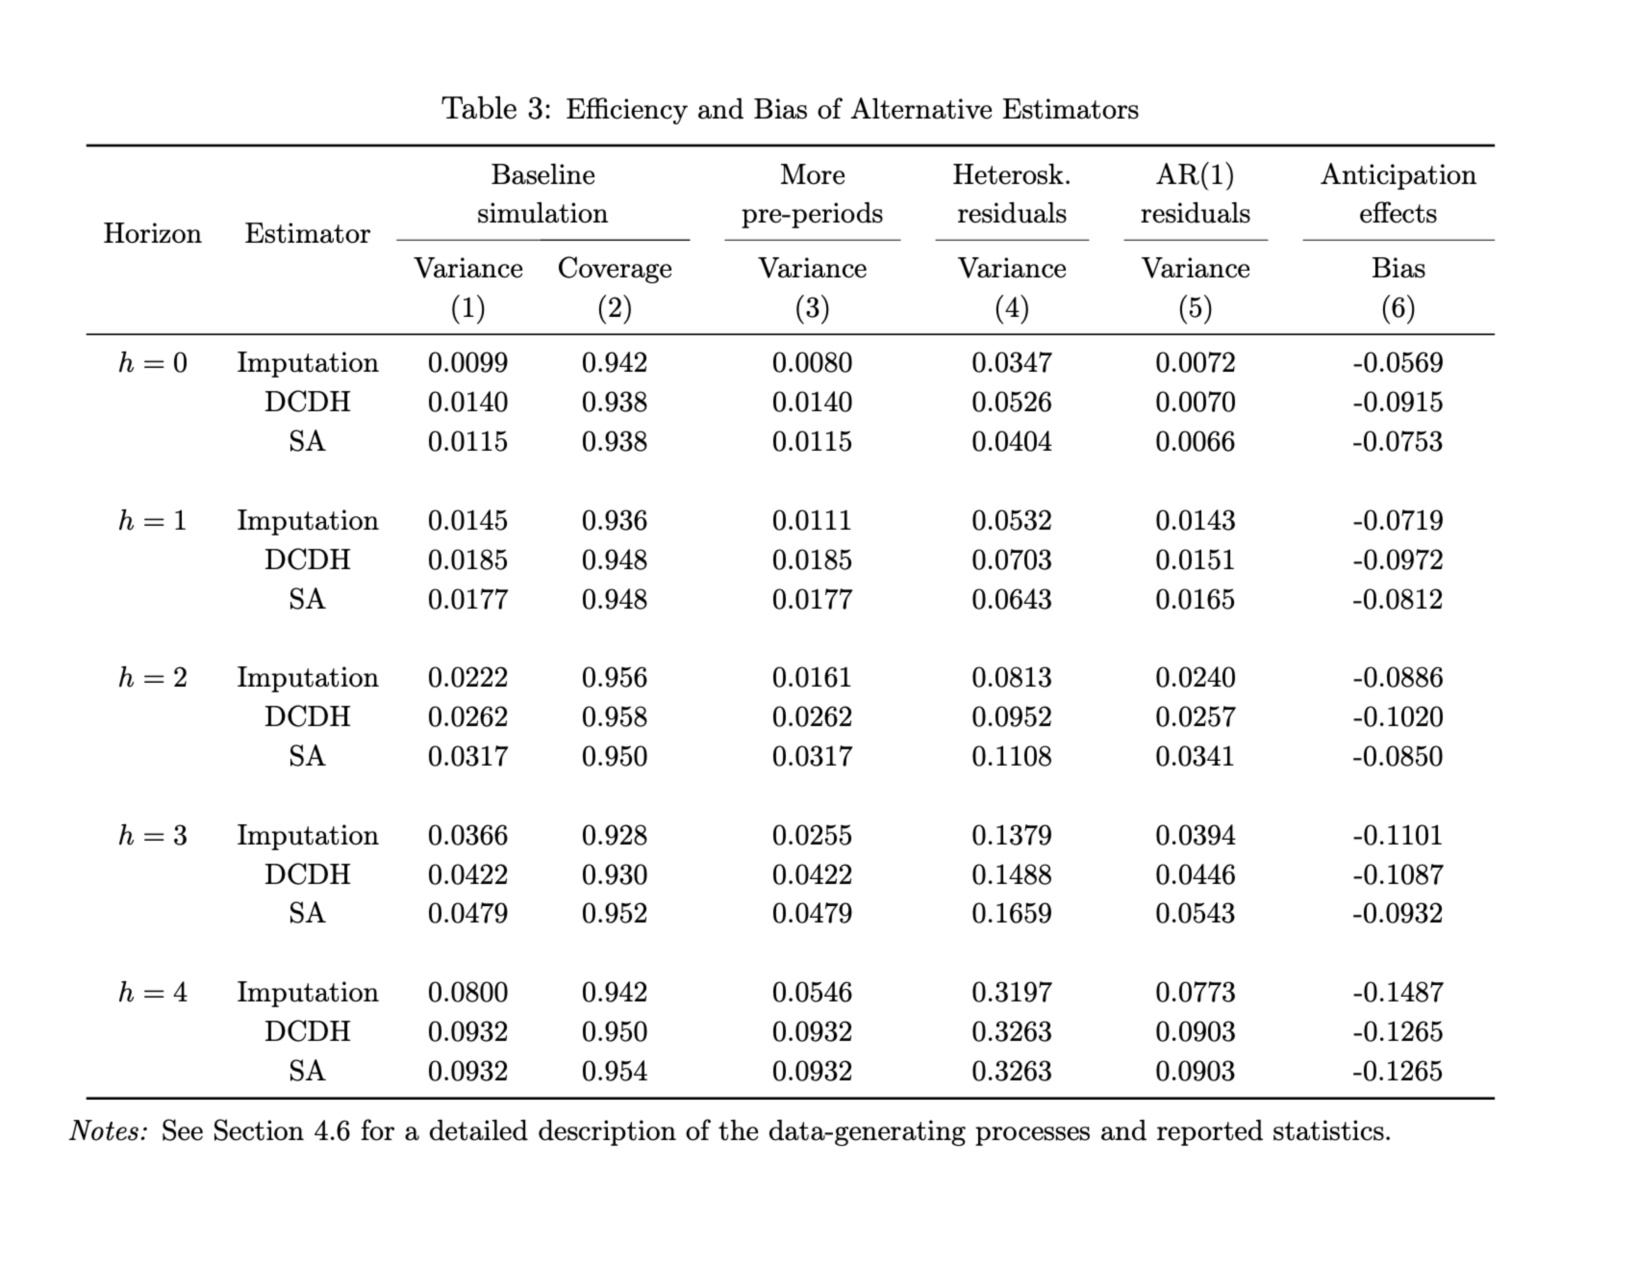
\includegraphics[scale=0.35]{./lecture_includes/bjs_sim.pdf}
\end{center}

\end{frame}


\subsection{2SDiD}

\begin{frame}{Two Stage DiD}

\begin{quote}
``It seems natural that TWFE should identify the ATT'' -- Gardner (2021)
\end{quote}

\bigskip

It just seems like TWFE with a DiD will estimate the ATT with weights that we'll find intuitive.  Was this just a conjecture and was never true?  Why isn't this working?

\end{frame}



\begin{frame}{Model misspecification}

\begin{itemize}
\item Why does TWFE fail under differential timing? Violates strict exogeneity under heterogeneity
\item The logic of the failure suggests an obvious, but previously unknown, solution which is the 2SDiD
\item ``Misspecified DiD regression models project heterogenous treatment effects onto group and period fixed effects rather than the treatment status itself''
\item If you can get consistent and unbiased estimates of group and relative time fixed effects, then you can delete them through residualizing the outcome and run normal analysis
\end{itemize}


\end{frame}


\begin{frame}{2SDiD}

\begin{itemize}
\item First stage -- estimate the group and relative time fixed effects using only the $D=0$ observations (like BJS)
\item Second stage -- using predicted values based off those fixed effect coefficients, run your model off the residualized outcome 
\item Get the standard errors right by taking the first stage into account (uses GMM)
\end{itemize}

\end{frame}

\begin{frame}{More high level}

\begin{itemize}
\item The second step recovers the average difference in outcomes between treated and untreated units after removing group and period fixed effects
\item Strong parallel trends assumption compared to CS and SA, but unclear if this is a big deal in general
\end{itemize}

\end{frame}

\begin{frame}{Notation}

$i$: panel units \\
$t$: calendar time -- think of real dates\\
$g\in \{0,1, \dots , G \}$ -- groups\\
$p \in \{0,1, \dots , P \}$  -- relative time or ``periods''\\

\bigskip

Periods are successive.  Group 0 -- never treated. Group 1 -- treated in period 1, 2, and on.  Group 2 -- treated in period 2, etc.

\end{frame}

\begin{frame}{Parameters}

\begin{eqnarray*}
\beta_{gp} = E \bigg [ Y^1_{gpit} - Y^0_{gpit} | g,p \bigg ]
\end{eqnarray*}

\bigskip

It's a group-time ATT but expressed in a more traditional econometric notation that you could easily find in Wooldridge or some such

\end{frame}

\begin{frame}{Modeling basics}

Under parallel trends, mean outcomes will satisfy the following equation

\bigskip

\begin{eqnarray*}
E \bigg [ Y_{gpit} | g,p,D_{gp} \bigg ] = \lambda_g + \gamma_p + \beta_{gp} D_{gp}
\end{eqnarray*}

\bigskip

In two-group, group and period effects are eliminated with dummies because TWFE uses dummies to demean across multiple dimensions. Then TWFE identifies ATT.  But this does not hold when average effects vary across group and period. There are many ways to express a treatment effect's across group and time, but Gardner presented it as a weighted average of the coefficients for only that group-period situation:

\begin{eqnarray*}
E \bigg (\beta_{gp} | D_{gp}=1 \bigg ) = E \bigg (Y^1_{gpit} - Y^0_{gpit} | D_{gp}=1 \bigg )
\end{eqnarray*}

\end{frame}


\begin{frame}{Strict exogeneity violation}

Rewriting the above we get:

\begin{eqnarray*}
E \bigg [ Y_{gpit} | g,p, D_{gp} \bigg ] &=& \lambda_g + \gamma_p + E \bigg [\beta_{gp} | D_{gp} =1 \bigg ] D_{gp} \\
&& \bigg [\beta_{gp} - E ( \beta_{gp} | D_{gp} = 1 ) \bigg ] D_{gp}
\end{eqnarray*}

\bigskip

The problem is there's this weird new error term and it isn't mean zero under heterogenous treatment effects spread across group and period.  Unlike the two group case, the coefficient on $D_{gp}$ from TWFE doesn't identify the average $E(\beta_{gp} | D_{gp}=1)$ 


\end{frame}

\begin{frame}{DiD regression estimand}

\begin{itemize}
\item So if TWFE isn't recovering $E(\beta_{gp} | D_{gp} = 1)$, then what is it recovering?
\item He shows that under PT, the coefficient on $D_{gp}$ is:

\begin{eqnarray*}
\beta^* = \sum_{g=1}^G \sum_{p=g}^P w_{gp}\beta_{gp}
\end{eqnarray*}

\item So then -- what are the weights $w_{gp}$?  They are variance weights 
\end{itemize}

\end{frame}

%\begin{frame}{Weights}

%\footnotesize
%\begin{eqnarray*}
%w_{gp} = \frac{ \bigg \{ [ 1-P(D_{gp}=1|g) ] - [P(D_{gp}=1|p) -  P(D_{gp}-1) ] \bigg \} P(g,p)}{
%\sum_{g=1}^G \sum_{p=g}^P \bigg \{ [ 1-P(D_{gp}=1 | g) ] - [P(D_{gp}=1 | p) - P(D_{gp}=1) ] \bigg \}P(g,p)}
%\end{eqnarray*}

%Terms: 
%\begin{itemize}
%\item $P(D_{gp}=1|p)$: share of units treated in period $p$
%\item $P(D_{gp}=1|g)$: share of periods in which $g$ is treated
%\item $P(D_{gp}=1)$: share of unit $\times$ time treated
%\item $P(g,p)$: population share of observation corresponding to group $g$ and period $p$
%\end{itemize}

%I thought about changing all those probabilities into means, but honestly, it really didn't help me at all.  But Gardner notes that this is from theorem 1 of deChaisemartin and D'Haultfoeiller (2020) and his Appendix A

%\end{frame}


\begin{frame}{Estimation}

\begin{eqnarray*}
Y_{gpit} = \lambda_g + \gamma_p + \beta D_{gp} + \varepsilon_{gpit}
\end{eqnarray*}

\bigskip

This specification assumes a conditional expectation function that is linear in group, period and treatment status.  But when the model is misspecified, it will attribute some of the heterogeneity impacts of the treatment to group and period fixed effects.  The longer the treatment, the greater $\overline{D}$ is, the more that group's treatment effects will be absorbed by group fixed effects.  When misspecified, TWFE doesn't recover $E[\beta | D=1]$.

\end{frame}

\begin{frame}{Statistical issues}

\begin{itemize}
\item Common support: ``as long as there are untreated and treated observations for each group and period, $\lambda_g$ and $\gamma_p$ are identified from the subpopulation of untreated groups and periods.''
\item Identification: ``the overall group $\times$ period ATT is identified from a comparison of mean outcomes between treated and untreated groups after removing group and period effects.''
\end{itemize}

\end{frame}


\begin{frame}{Estimation: First stage}


First stage:
\begin{eqnarray*}
Y_{gpit} = \lambda_g + \gamma_p + \varepsilon_{gpit}
\end{eqnarray*}using only $D_{gp}=0$, retaining the fixed effects. Collect the $\widehat{\lambda_g}$ and $\widehat{\gamma_p}$.

\end{frame}

\begin{frame}{Estimation: Second stage}

Second stage:
\begin{eqnarray*}
\widehat{y}_{gpit} &=& y_{gpit} - \widehat{\lambda_g} - \widehat{\gamma_p} \\
\widehat{y}_{gpit} &=& \alpha + \beta D_{gp} + \psi_{gpit}
\end{eqnarray*}Why does this work? Parallel trends assumption implies:

\bigskip

\footnotesize
\begin{eqnarray*}
E(y_{gpit} | g,p,D_{gp}) - \lambda_g - \gamma_p = E \bigg [ \beta_{gp} | D_{gp}=1 \bigg ] D_{gp} + \bigg [ \beta_{gp} - E(\beta_{gp} | D_{gp}=1) \bigg ] D_{gp}
\end{eqnarray*}But because

\begin{eqnarray*}
E \bigg \{ [ \beta_{gp} - E( \beta_{gp} | D_{gp} =1) ] D_{gp} | D_{gp} \bigg \} = 0
\end{eqnarray*}


\end{frame}

\begin{frame}{Estimand}

Then this procedure will identify $E(\beta_{gp} | D_{gp}=1)$. Consistency and unbiasedness proofs. 

\bigskip

This is $E(\beta_{gp}|D_{gp}=1) = \sum^G \sum^P \beta_{gp} P(g,p|D_{gp}=1)$. It will tend to put more weight, by definition, on groups earlier into their treatment.  But this isn't the same as the negative weighting that BJS say occurs oof the long lags.  It just means there are more of them.

\bigskip

Event studies are:
\begin{eqnarray*}
y_{gpit} = \lambda_g + \gamma_p + \sum_{r=-R}^P \beta_rD_{rgp} + \varepsilon_{gpit}
\end{eqnarray*}Just change the second stage with the transformed outcome. 

\end{frame}

\begin{frame}{Inference}

\begin{itemize}
\item Standard errors are wrong on the second stage because the dependent variable uses estimates obtained from the first stage. 
\item The asymptotic distribution of the second stage can be obtained by interpreting the two-stage procedure as a joint GMM
\end{itemize}

\end{frame}

\section{Examples}


\subsection{Facebook and Mental Health}


\begin{frame}{Motivation}

\begin{itemize}
\item Widely cited that social media causes mental health problems in youth but no causal evidence (``slim to none'')
\item Braghieri, Levy and Makarin (2022), ``Social Media and Mental Health'', \emph{American Economic Review}, 112(11): 3660-3693
\item Study will use staggered rollout of Facebook platform to college campuses from 2004 to 2006 to estimate the effect on aggregate mental health scores from a survey

\end{itemize}

\end{frame}



\begin{frame}{Fourth part of a strong DiD}

\begin{enumerate}

\item \textbf{Bite}: They cannot really show much here.  No data on Facebook usage.  More an ITT
\item \textbf{Falsifications}: Interestingly, they dod none
\item \textbf{Event studies}: Now canonical kind of presentation of main results
\item \textcolor{red}{Mechanism}: Weakly suggestive (you decide)

\end{enumerate}

\end{frame}






\begin{frame}{Outcome Data}

\begin{itemize}

\item Long-running health survey conducted at colleges in the US
\item Requested that the survey owners match their facebook data with the survey data
\item They said yes and did it but then never returned any calls (though the DUA had been signed)
\item Outcomes are normalized so that coefficients on treatment is in standard deviations (e.g., z-score)
\end{itemize}

\end{frame}

\begin{frame}{Treatment Data and Wayback machine}

\begin{itemize}

\item Used Wayback machine from when it was \url{thefacebook.com}
\item Identified all schools in the data by looking at each each front page to identify precise dates of rollout
\end{itemize}

\end{frame}

\begin{frame}{Treatment Data and Wayback machine}
\begin{center}

\includegraphics[scale=0.35]{./lecture_includes/timemachine_1}
\end{center}
\end{frame}

\begin{frame}{Treatment Data and Wayback machine}
\begin{center}

\includegraphics[scale=0.35]{./lecture_includes/timemachine_2}
\end{center}
\end{frame}


\begin{frame}{TWFE}

\begin{equation}
Y_{icgt} = \alpha_g + \delta_t + \beta \times Facebook_{gt} + X_i \times \gamma + X_c \times \psi + \varepsilon_{icgt}
\end{equation}

\bigskip

Their primary model is TWFE -- done largely to appease referees


\end{frame}



\begin{frame}
\begin{center}
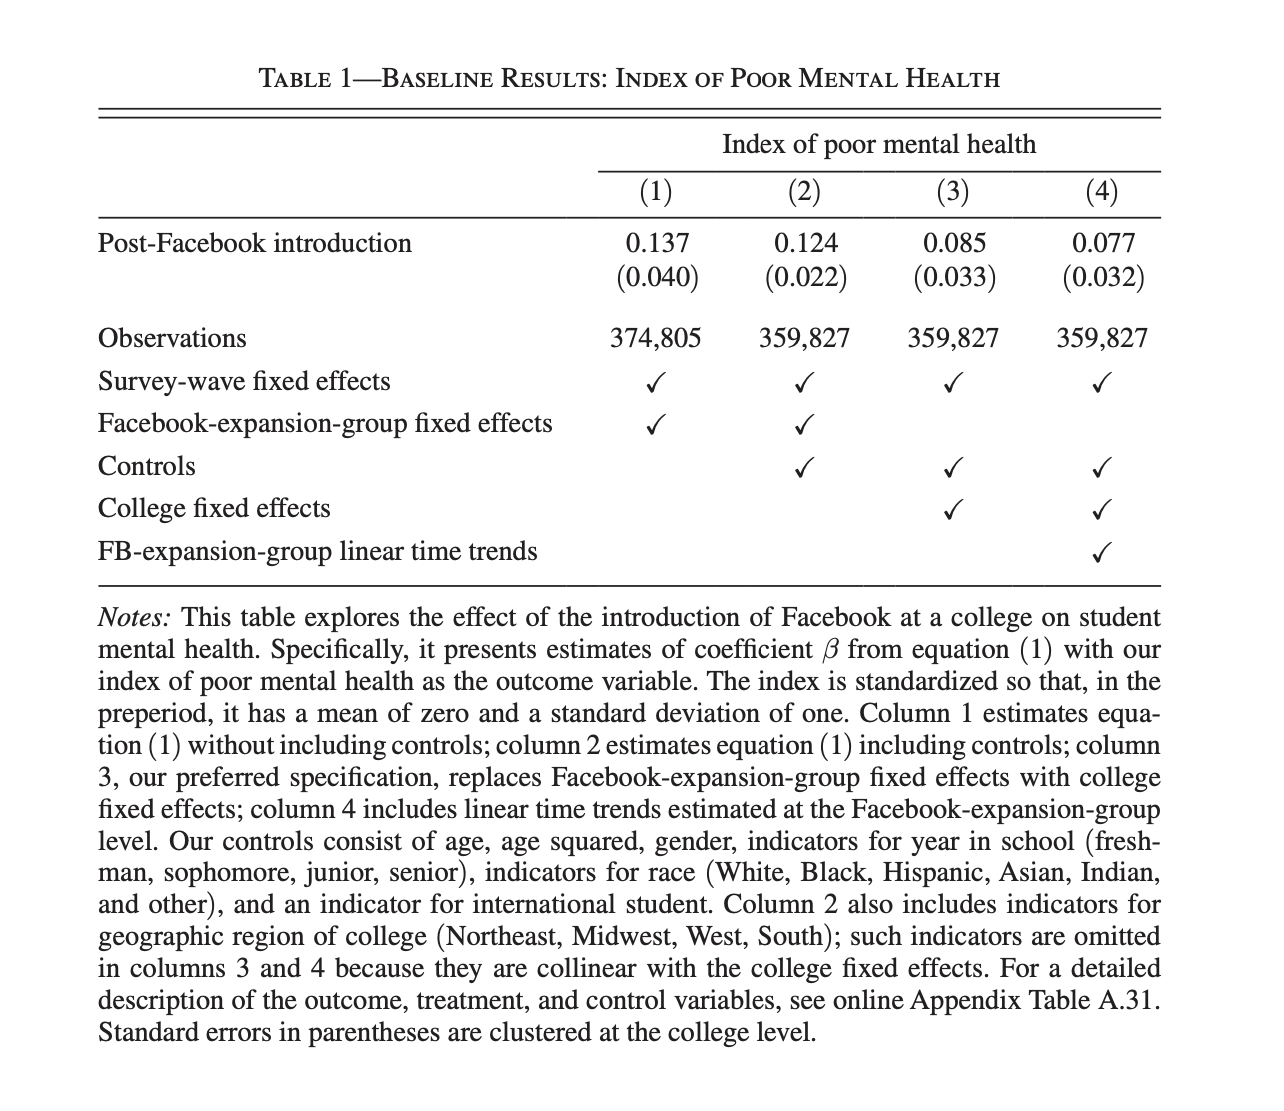
\includegraphics[scale=0.35]{./lecture_includes/facebook_1}
\end{center}
\end{frame}

\begin{frame}
\begin{center}
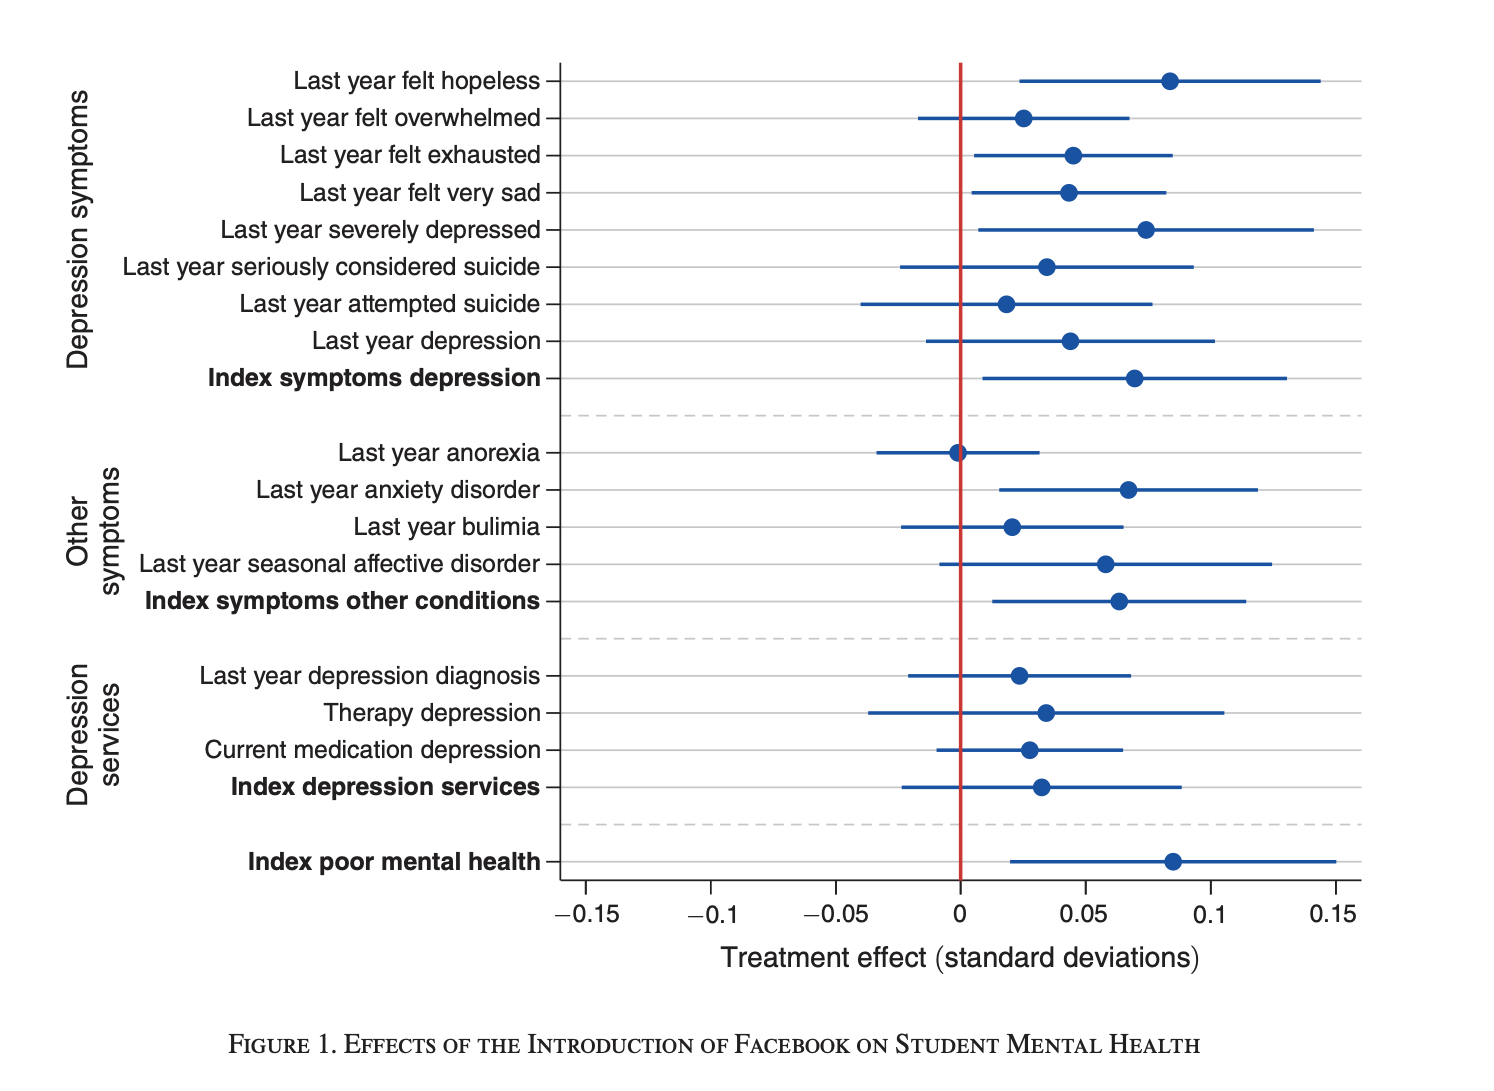
\includegraphics[scale=0.35]{./lecture_includes/facebook_2}
\end{center}
\end{frame}

\begin{frame}
\begin{center}
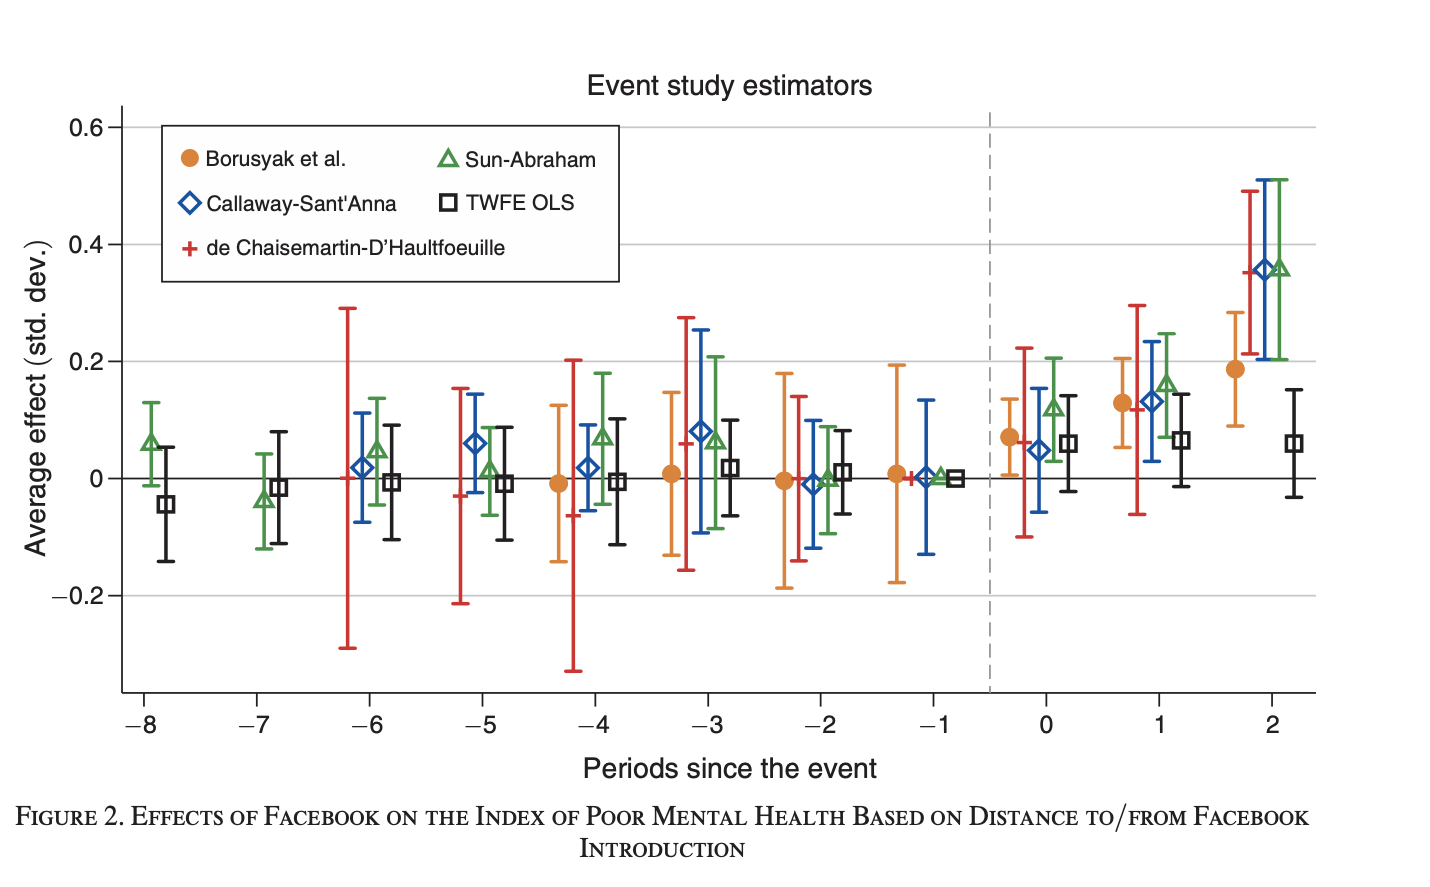
\includegraphics[scale=0.35]{./lecture_includes/facebook_3}
\end{center}
\end{frame}

\begin{frame}
\begin{center}
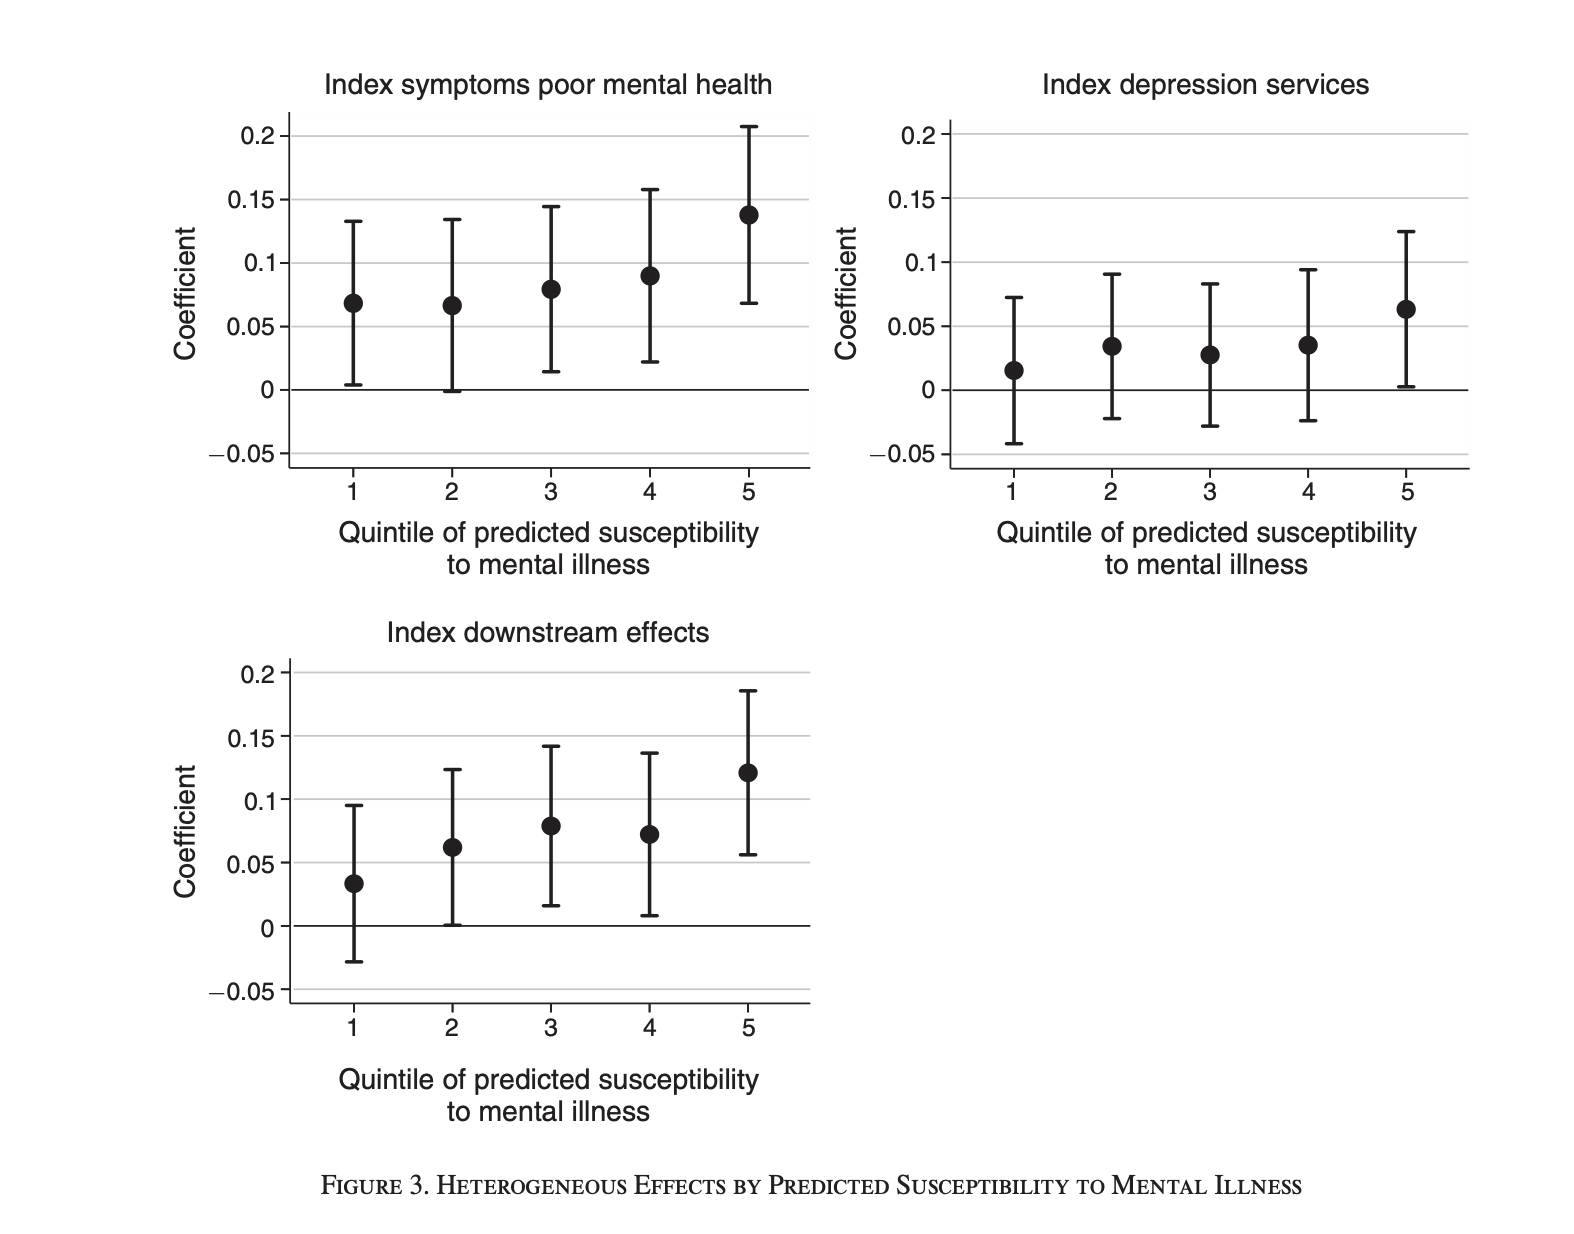
\includegraphics[scale=0.35]{./lecture_includes/facebook_4}
\end{center}
\end{frame}

\begin{frame}
\begin{center}
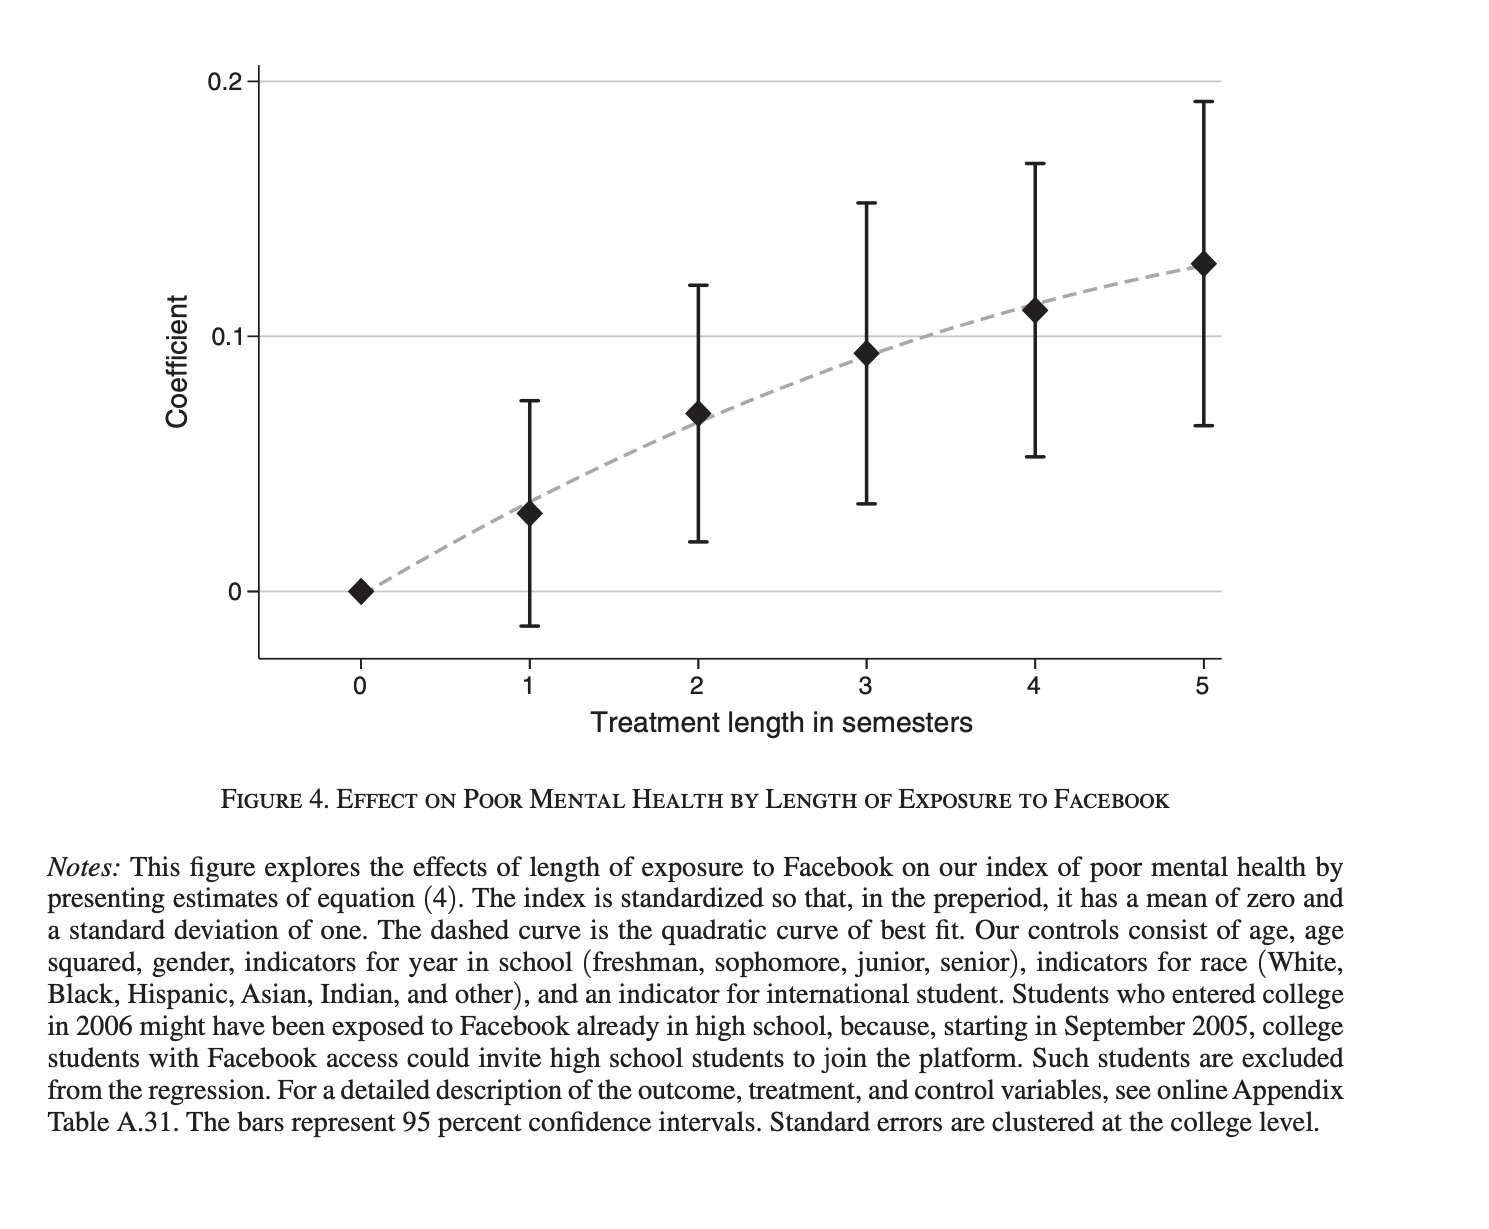
\includegraphics[scale=0.35]{./lecture_includes/facebook_5}
\end{center}
\end{frame}

\begin{frame}
\begin{center}
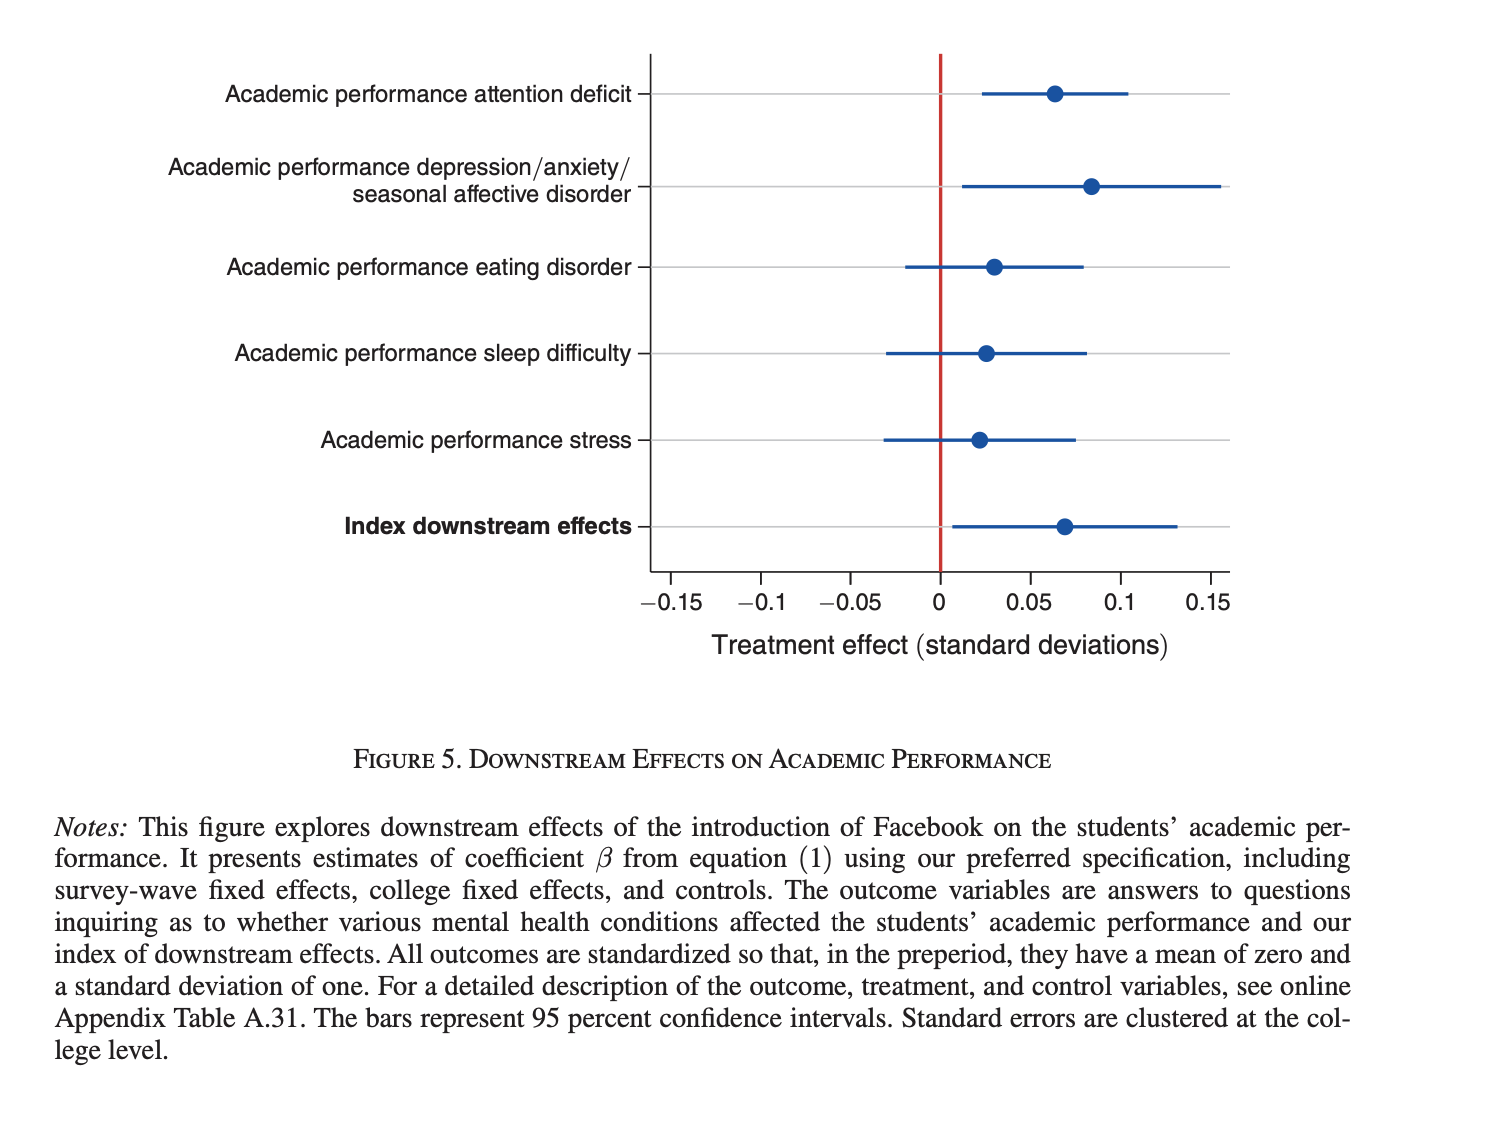
\includegraphics[scale=0.35]{./lecture_includes/facebook_6}
\end{center}
\end{frame}

\begin{frame}
\begin{center}
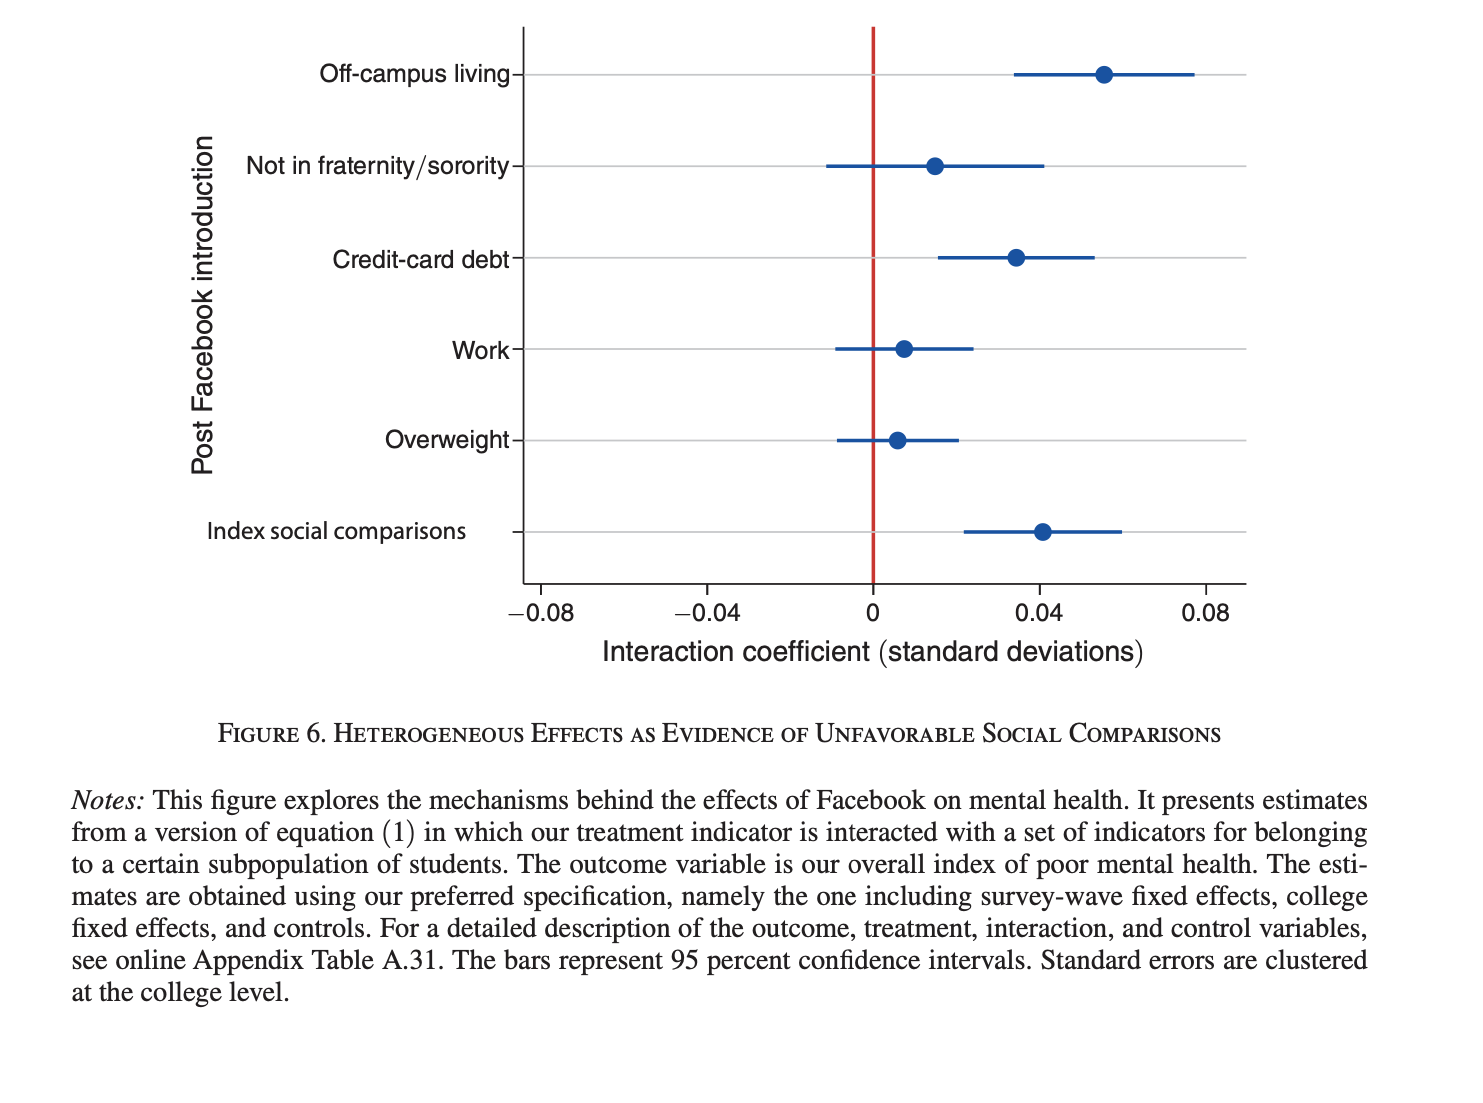
\includegraphics[scale=0.35]{./lecture_includes/facebook_7}
\end{center}
\end{frame}










\subsection{Castle doctrine}


\begin{frame}{Case study: Castle doctrine reforms}

\begin{itemize}
\item We will replicate this together
\item Cheng and Hoekstra (2013) is a good, clean example of a differential timing for us to practice on
\item In 2005, Florida passed a law called Stand Your Ground that expanded self-defense protections beyond the house
\item More ``castle doctrine'' reforms followed from 2006 to 2009

\end{itemize}

\end{frame}

\begin{frame}{Description}

Details of castle doctrine reforms
		\begin{itemize}
		\item ``Duty to retreat'' is removed versus castle doctrine reforms; expanded where you can use lethal force
		\item Presumption of reasonable fear is added
		\item Civil liability for those acting under the law is removed
		\end{itemize}
\end{frame}

\begin{frame}{Ambiguous predictions}
	
Castle reforms $\rightarrow$ homicides: Increase by removing homicide penalties and increasing opportunities
	\begin{itemize}
	\item Castle doctrine expansions lowered the (expected) cost of killing someone in self-defense
	\item Lowering the price of lethal self-defense should increase lethal homicides
	\end{itemize}
\bigskip
Castle reforms $\rightarrow$ homicides: decrease through deterrence

\end{frame}


\begin{frame}{Cheng and Hoekstra's estimation model}
	
	\begin{itemize}
	\item TWFE model$$Y_{it} = \beta_1 D_i + \beta_2 T_t + \beta_3 (CDL_{it}) + \alpha_1X_{it} + c_i + u_t + \varepsilon_{it}$$
	\item $CDL$ is a fraction between 0 and 1 depending on the percent of the year the state has a castle doctrine law 
	\item Preferred specifications includes ``region-by-year fixed effects'' (see next slide)
	\item Estimation with TWFE and Poisson with and without population weights
	\item Models will include covariates (e.g., police, imprisonment, race shares, state spending on public assistance)
	\end{itemize}
\end{frame}


\begin{frame}{Publicly available crime data}
	
Main data: FBI Uniform Crime Reports Part 1 Offenses (2000-2010)
		\begin{itemize}
		\item Main outcomes: log homicides
		\item Falsification outcomes: motor vehicle theft and larceny (skipping this)
		\item Deterrence outcomes: burglary, robbery, assault
		\end{itemize}
\end{frame}



\begin{frame}{Region-by-year fixed effects}
	
	\begin{itemize}
	\item \textbf{Parallel trends assumption}: imposed structurally with region-by-year dummies
	\item \textbf{Argument}: unobserved changes in crime are running ``parallel'' to the treatment states within region over time
	\item \textbf{SUTVA} and \textbf{No Anticipation}: No spillovers, no hidden variation in treatment, no behavioral change today in response to tomorrow's law
	\end{itemize}
\end{frame}



\begin{frame}{Results -- Deterrence}
	
	\begin{figure}
	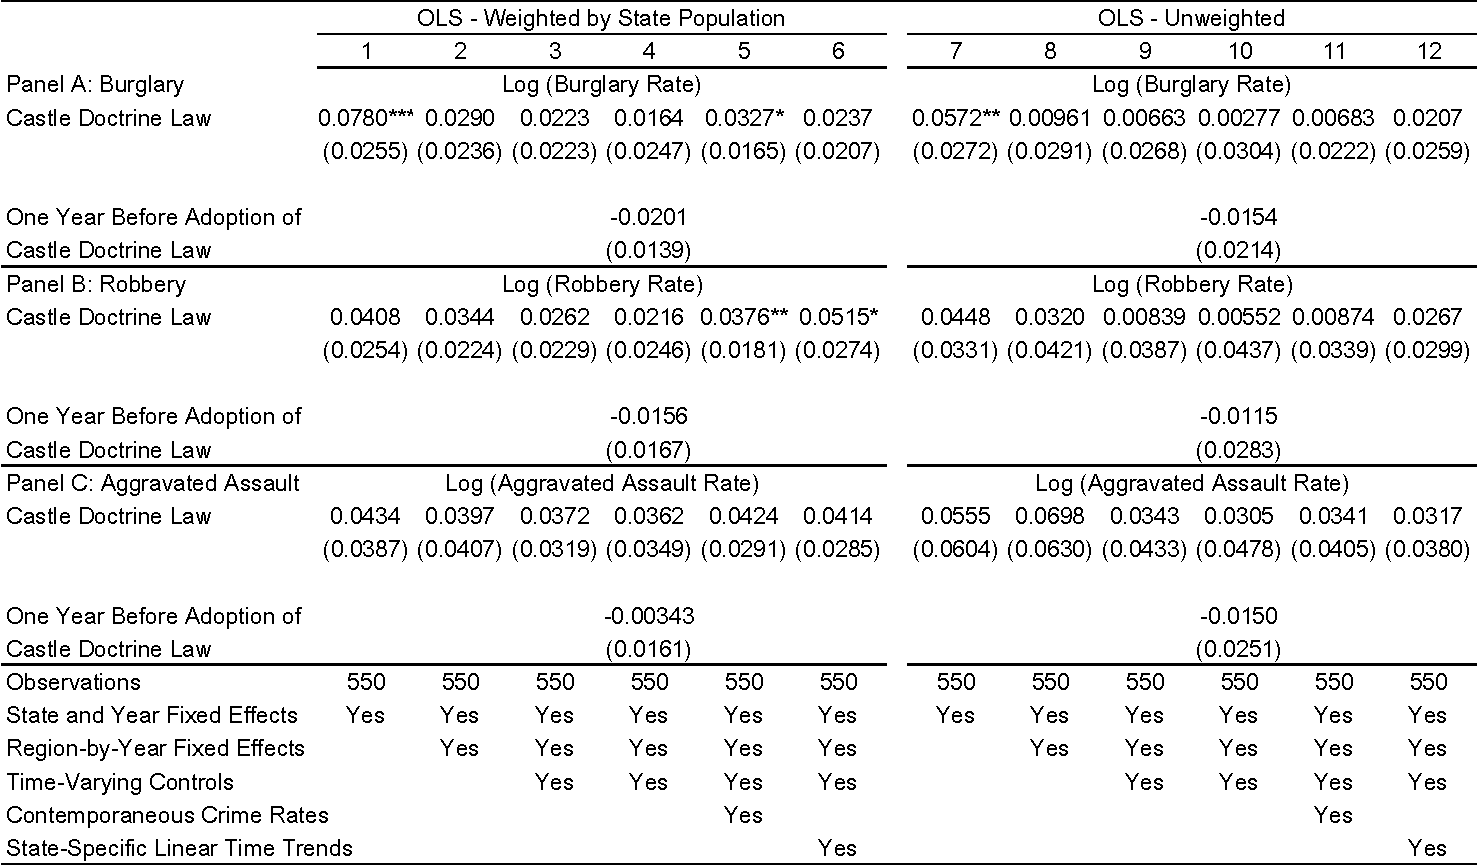
\includegraphics[scale=0.4]{./lecture_includes/cheng4.pdf}
	\end{figure}
\end{frame}




\begin{frame}{Results -- Homicides}
	
	\begin{figure}
	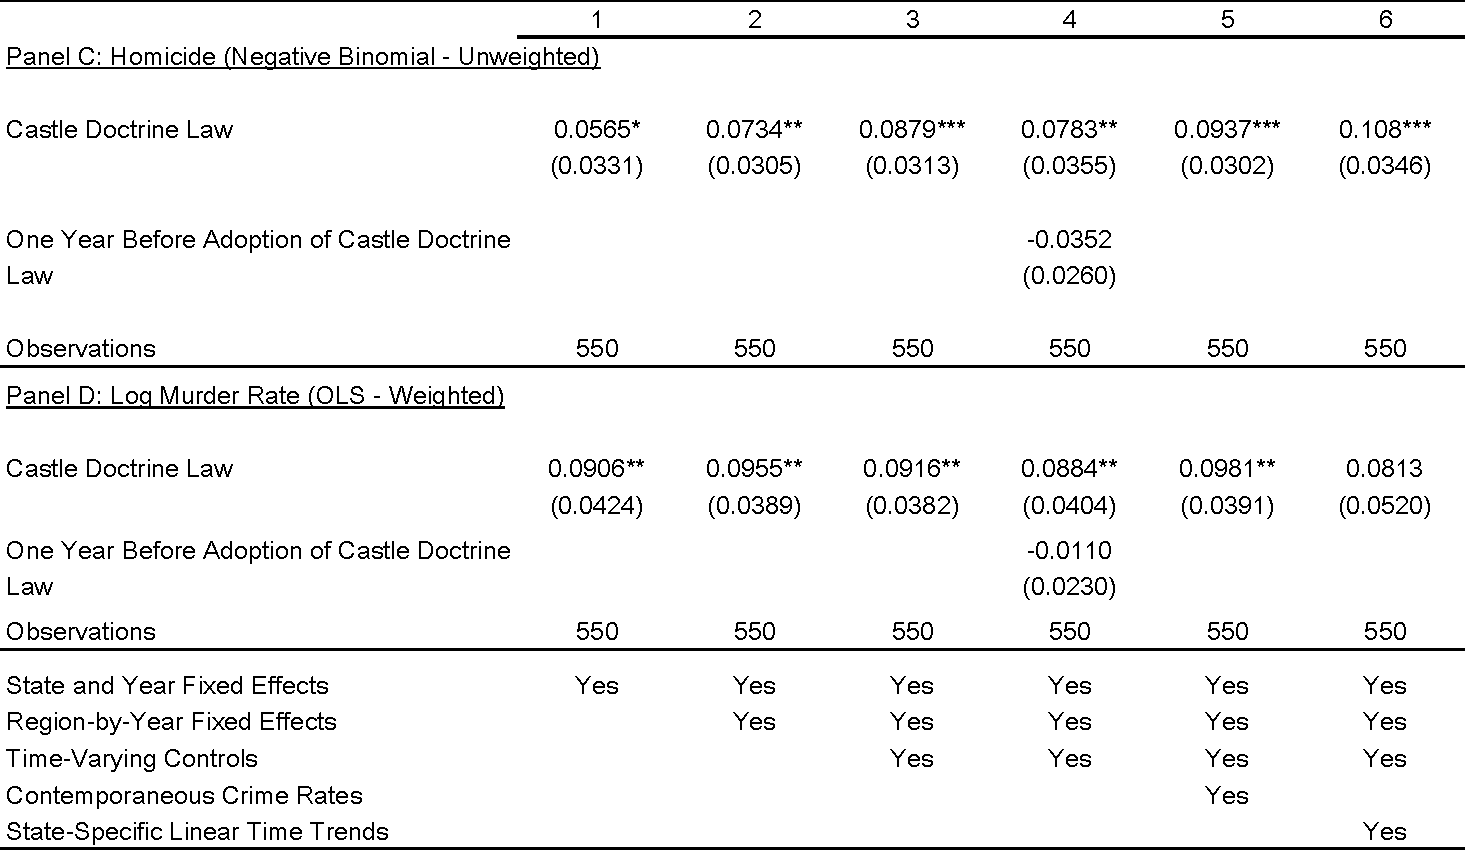
\includegraphics[scale=0.4]{./lecture_includes/cheng12.pdf}
	\end{figure}
\end{frame}



\begin{frame}{Interpretation}
	
	\begin{itemize}
	\item Series of robustness checks (falsifications on larceny and motor vehicle theft; deterrence; many different specifications)
	\item Castle doctrine reforms are associated with an 8\% net increase in homicide rates per year across the 21 adopting states
	\item Interpretation is these would not have occurred without castle doctrine reforms
	\item But is this robust to alternative models? Today we will check
	\end{itemize}
\end{frame}





\section{Basic suggestions going forward}


\begin{frame}{Robust DiD is now standard practice}

\begin{itemize} 
\item You're probably going to write a paper using DiD at least once in your life, but probably more
\item Even if you don't, you're going to read a lot of papers using DiD, referee them, or advise students using them
\item It's in your best interest to make the fixed cost investment in the new econometrics of DiD because the old methods are mostly harmful
\item Good news is we are at the conclusion of this wave of papers, software is now widely available, solutions tend to have common features, and overall presentations (static and dynamic) aren't all that different
\end{itemize}

\end{frame}

\begin{frame}{Handling covariates may need some finesse}

\begin{itemize}
\item Simple 2x2 has its own problems when estimated using TWFE \emph{if you include covariates}
\item Stronger assumptions needed to include covariates, and bias can be large
\item Don't control for covariates that could be affected by the outcome 
\end{itemize}

\end{frame}

\begin{frame}{Avoid forbidden contrasts}

\begin{itemize}
\item Main problem in differential timing is heterogeneity and the use of already-treated units as controls 
\item TWFE hid this under the hood more than likely
\item Under differential timing, canonical TWFE assumes constant treatment effects and without it is biased (and can even flip signs)
\item Robust DiD methods do not place restrictions on treatment effect heterogeneity 
\end{itemize}

\end{frame}

\begin{frame}{Moving to synthetic control}

\begin{itemize}
\item When you lose parallel trends, you're probably going in the direction of needing synthetic control methods
\item There are plenty and they also require good form fit pre-treatment
\item But when you fail that, there are new advances -- augmented synth, Imbens and Doudchenko both allow for lower quality fit
\end{itemize}

\end{frame}








\end{document}

